
\documentclass[conference]{IEEEtran}

%\usepackage{ifpdf}
\usepackage{float}  % For handling float environments like [H]
\usepackage{url}    % For handling URLs
\usepackage{multirow}
\usepackage{subcaption} % Required for subfigures
\usepackage{booktabs}
\usepackage{cite}
\pagestyle{plain}
\usepackage{amsmath}
\usepackage{float}
\usepackage{tikz}
\usetikzlibrary{shapes.geometric, arrows, positioning}%\usepackage{url}
\usepackage{placeins}


\ifCLASSINFOpdf
  \usepackage[pdftex]{graphicx}
  % declare the path(s) where your graphic files are
  % \DeclareGraphicsExtensions{.pdf,.jpeg,.png}
%\else
  % or other class option (dvipsone, dvipdf, if not using dvips). graphicx
  % and their extensions so you won't have to specify these with
  % every instance of \includegraphics
  % \DeclareGraphicsExtensions{.eps}
\fi
% graphicx was written by David Carlisle and Sebastian Rahtz.


% correct bad hyphenation here
\hyphenation{op-tical net-works semi-conduc-tor}


\begin{document}


\title{Applying Machine Learning Models to Assess Fatigue and Prevent Injury in High Performance Swimming Athletes}

% use a multiple column layout for up to three different
% affiliations
\author{\IEEEauthorblockN{\\ Hugo Veríssimo}
\IEEEauthorblockA{Foundations of Machine Learning 24/25\\
University of Aveiro\\
Aveiro, Portugal\\
hugoverissimo@ua.pt}
\and
\IEEEauthorblockN{\\ João Cardoso}
\IEEEauthorblockA{Foundations of Machine Learning 24/25\\
University of Aveiro\\
Aveiro, Portugal\\
joaopcardoso@ua.pt}}


% make the title area
\maketitle
\thispagestyle{plain}


% As a general rule, do not put math, special symbols or citations
% in the abstract
\begin{abstract}
Improving performance of elite athletes is the ultimate goal of any sports coach. For proper planning and continued improvement, a good balance between workload and rest is crucial. There are several metrics used to assess the impact of the workload that athletes are subject of, with the rate of perceived exertion being amongst the most relevant throughout decades of research in the field. 
For this project the authors used data from the 2019/2020 season from the local swimming club CAPGE, provided by Head Coach Daniel Tavares, in order to develop machine learning models for fatigue prediction. The data consisted of athlete's feedback and training load, of which a set of features was selected and average over different periods. The models used were logistic regression, support vector machine, and decision tree. Overall the models performed decently, with support vector machine standing out as the best performing. 
The model developed was documented and shared in Excel format for practical application, and will be followed up with further data collection.
\end{abstract}

\begin{quote}
\small
\noindent
\textbf{Keywords:} swimming, fatigue prediction, logistic regression, support vector machine, decision tree
\end{quote}

\IEEEpeerreviewmaketitle


\section{Introduction}
The evolution in performance of high level athletes is highly dependent on their skill, motivation, and discipline. With the support of a knowledgeable coach, the evolution can be substantially improved, through careful tailoring of the training regimen. One of the most relevant metrics since the beginning of structured training in sports is the feedback from the athlete, commonly described as the rate of perceived exertion (RPE). This single metric comprises the athletes analysis and intuition of the effort that was carried and how ready they feel for the next session of training. In recent years, more and more sports coaches have relied heavily on collected data to better assess, plan and adjust the training plans of their athletes in a systematic way. This allows for a fine balance between intense workouts, that generate stronger stimuli for muscle development and sport specific skills, taking the balance between effort and fatigue as the crucial ratio to respect. Too high effort, may lead to injury, too low and some gains may be left on the Table \cite{Zatsiorsky2019}. 

In the scope of the first project for Foundations of Machine Learning, the authors decided to partner with a local sports club CAPGE (Clube Associação de Pais da Gafanha da Encarnação) to process the data (kindly shared by Head Coach Daniel Tavares), to develop a general machine learning (ML) model for estimating the fatigue in swimming athletes. The data was curated and prepared to be fit through different machine learning algorithms to estimate fatigue after workout.

With this approach, the goal is to generalize the models for different athletes/sports, and make it available to the local club for implementation and further testing. 



\section{State of the Art}

Over the past decade there have been significant improvements in the field of ML applied algorithms for sports' related applications. The most relevant work in fatigue and injury prediction is briefly discussed in the present section, which is not specifically on the sport assessed in this project, which lead to additional interpretations from the works analyzed to our own case of study. In general, the problem of class imbalance is seen throughout the literature, and different solutions are proposed, such as data gathering and preprocessing, over sampling and under sampling, with SMOTE (synthetic minority over-sampling technique) being the most commonly used approach for over sampling \cite{Rossi2022}. As early as 2010, Gabbet and colleagues modeled the risk of injury with a monodimensional approach using logistic regression, based on athletes rate of perceived exertion, showing that even with a monovariate approach to injury prediction useful results could be attained \cite{Gabbett2010}. In recent years, several authors have focused in alternative techniques such as Logistic Regression \cite{murray2017calculating}, Random Forest \cite{Vallance2020}, Support Vector Machine \cite{Carey_2018}, or Convolutional Neural Network on Multivariate Timeseries \cite{pappalardo2019explainable}.

Besides model selection, feature engineering and selection is among the most debated topics. Several authors opt to include GPS data, metabolic consumption, mechanical load, RPE, detailed quantification of workloads, ratio between acute:chronice loads. Despite the multivariate imputation, data analysis often shows strong correlations between them, leading to overfitting problems (usually model independent) \cite{Rossi2022}.

In the work by Carey et al. (2018) different algorithms have been implemented to predict the risk of injury in an Australian football club. The data collection lasted for three seasons, consisting of absolute and relative training load metrics, derived from GPS, accelerometer, and RPE data. The prediction models used were regularized logistic regression, generalized estimating equations, random forests, and support vector machines, with periods of 3, 6, and 21 days (these periods have been studied and verified as adequate for the case of Australian football). The periods served to calculate moving averages and exponentially weighted moving averages (EWMA). The latter allowed to account for the decay in significance of the training load the further it happened from a given day, in accordance with the work from Williams et al. (2016). From the results it was possible to verify that overfitting was very likely due to the multicollinearity between variables, which was confirmed by principal component analysis (PCA). The use of PCA with regularized logistic regression slightly improved the results \cite{Carey_2018}.

More recent studies have employed ensemble algorithms, in order to take most of the different learning models selected, taking into account the need to balance the classes as is common practice for this type of problems \cite{lopez2018preventive}. 

In summary, the integration of machine learning techniques in sports fatigue and injury prediction has evolved from simple monovariate models to complex multivariate and ensemble approaches. Addressing challenges such as class imbalance, feature selection, and multicollinearity remains crucial for developing robust predictive models applicable across different sports contexts.

\section{Methodology}

The methodology for this project consisted of three major steps: assessment and curation of the dataset, feature engineering and selection of features, followed by data normalization; training of the selected machine learning models; finalizing with model evaluation and subsequent training until optimum results were achieved. Fig.~\ref{fig:methodology} illustrates the methodology used in this project.

\begin{figure}[h]
\centering
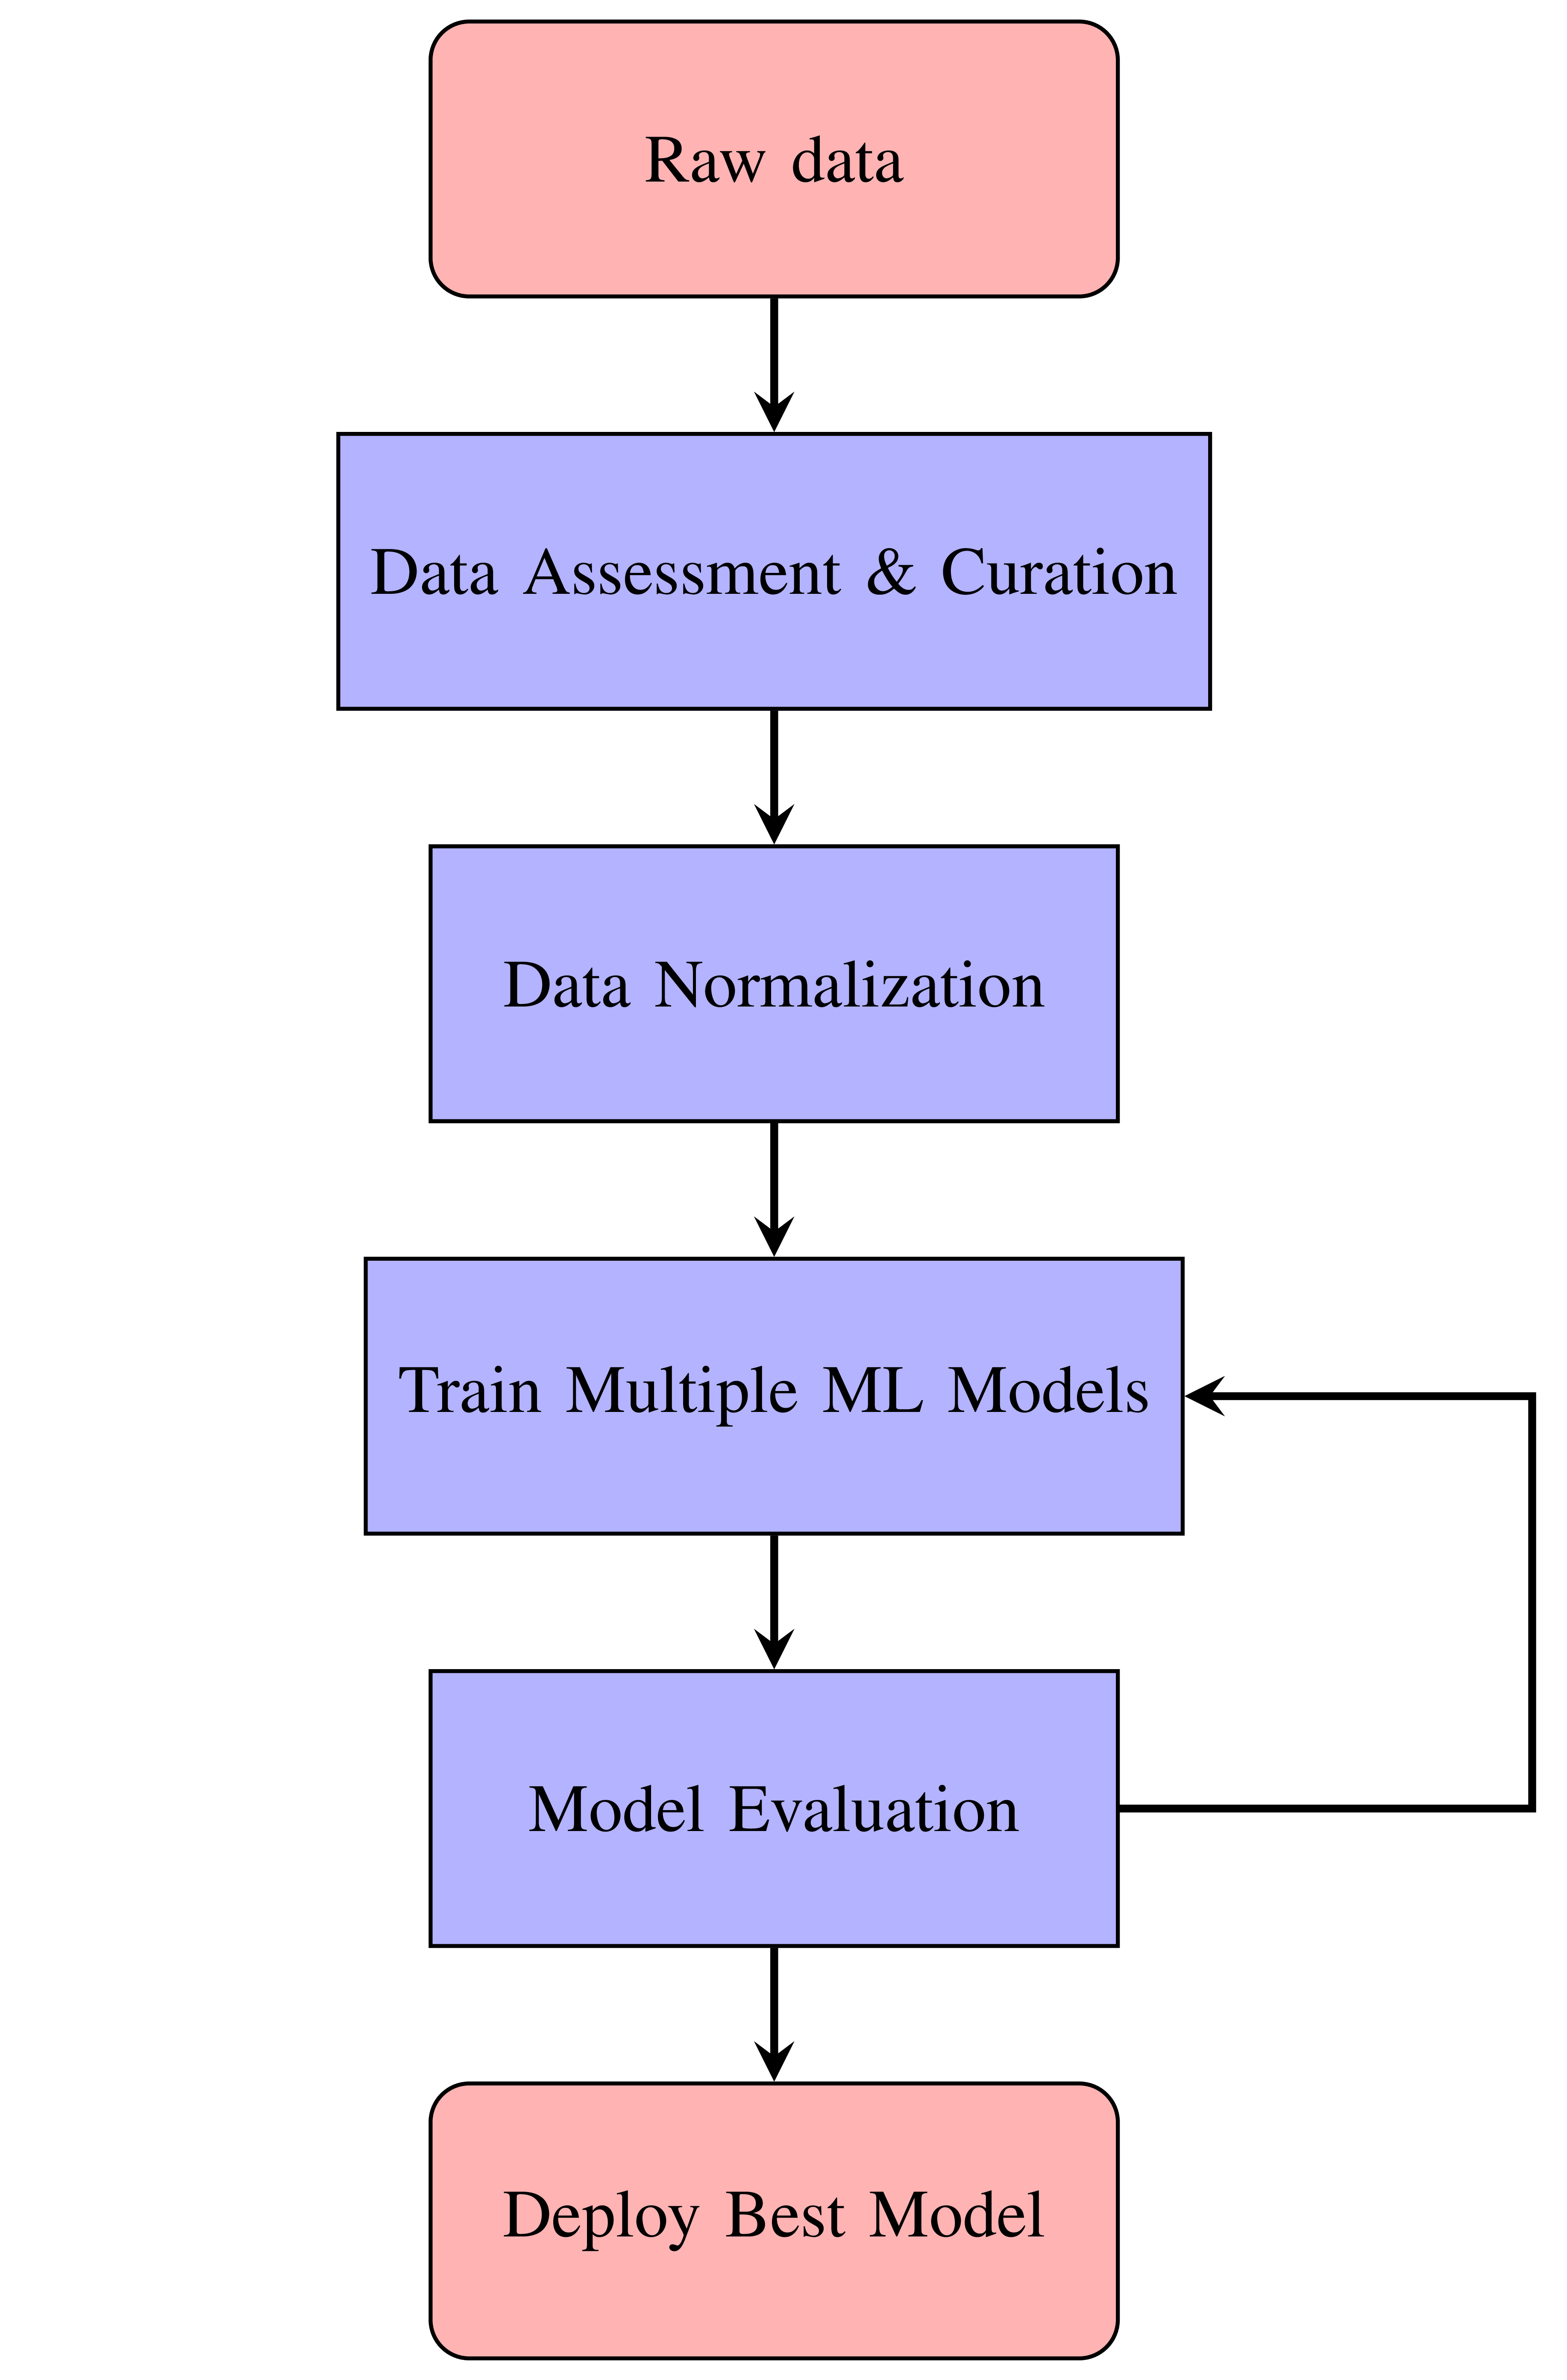
\includegraphics[width=0.72\linewidth]{assets/fluxog.png}
\caption{Flowchart of the methodology for data processing and modeling. The evaluation results are used to refine the model training process.}
\label{fig:methodology}
\end{figure}

The programming language used was Python, and the packages available therein, with notable mention for \texttt{scikit-learn} \cite{scikit-learn}. After data normalization for all features (using \texttt{StandardScaler}), the data was separated between training and testing data (80/20, respectively), using the \texttt{train\_test\_split} function from \texttt{sklearn}. The seeds for randomization were kept consistent across models, to ensure reproducibility, and avoid biases towards any model. 
The ML models selected for the project were Logistic Regression (LogReg), Support Vector Machine (SVM), and Decision Tree Classifier (DTree), where the modeling approach and hyperparameters are detailed throughout. For the given hyperparameters available in each model the function \texttt{RandomizedSearchCV} was used, to optimize the model, with 8-fold cross-validation, to minimize the risk of overfitting (the selected 8-fold CV was consistent throughout all the relevant stages, class weight estimation, training). 

The metrics used to assess the different models are presented in Table \ref{evaluationmetrics}, and are consistent with those used in the literature.

\begin{table}[H]
\centering
\caption{Metrics for multiclass classification model evaluation.}
\label{evaluationmetrics}
\begin{tabular}{lc}
\toprule
\textbf{Measure} & \textbf{Formula} \\
\midrule
Precision (per class $i$) & $\dfrac{TP_i}{TP_i + FP_i}$ \\[1em]
Recall (per class $i$) & $\dfrac{TP_i}{TP_i + FN_i}$ \\[1em]
F1-score (per class $i$) & $2 \cdot \dfrac{\text{Precision}_i \cdot \text{Recall}_i}{\text{Precision}_i + \text{Recall}_i}$ \\[1em] 
Accuracy & $\dfrac{\sum_{i=1}^{C} TP_i}{\sum_{i=1}^{C} (TP_i + TN_i + FP_i + FN_i)}$ \\[1em]
\bottomrule
\end{tabular}
\end{table}

Given the class imbalance associated with the problem at hand, the importance of precision, recall and F1-score per class are especially relevant, along with the confusion matrix, to understand how the model is failing to correctly classify the various observations. The precision is the ratio of true positives for all the positives attributed (the higher, the better). Recall (or sensitivity) gives the ratio of true positives among true positives and false negatives, where lower values indicate a higher number of misidentified true positives. The F1-score provides a balanced assessment of the model, taking a harmonic mean of precision a recall, providing a particularly good way to assess datasets with imbalanced classes, while accuracy provides an overall assessment with the ratio of true positives and true negatives over the total predictions.

The learning curve was used for all models, to highlight the relation between the size of the training dataset and the performance of the adjusted model, providing a good insight into the quality of the fitting. In the case of increasing accuracy of the training curve while the validation curve remains constant or decreases below the training curve, is a clear sign of overfitting. In the case that both curves converge, but to low values (below 0.6) is a sign of under fitting and poor learning from the model.

The confusion matrix was used to assess the performance in estimating each class during training and testing, giving a clear idea how the model is trying to predict the classes, helping to better interpret the class weights attributed.

The methods and ML models used are consistent with those in the literature, considering the type of features and target in this project. Moreover, during the model refinement stage a reassessment of past steps was carried in order to ensure no gaps in the process. 

\section{Dataset Analysis}

\subsection{Data Description}

The data used in this project was collected from the swimming club CAPGE during the season of 2019/2020, where each athlete has several observations corresponding to training days, where each of the features was collected. Not all athletes logged the same number of training days, nor present an equal distribution between low, average and high levels of intense training. The names of the athletes were removed to ensure privacy and confidentiality, keeping only the gender as a variable. The team is comprised by seven athletes, three male and four female. Most of the features are related to feedback from the athletes on different aspects of their lives (i.e. sleep quality, appetite, and rate of perceived exertion after training), while others are measurable (i.e. workload, variation in heart rate before and after training, weight variation). A notable feature to mention is the RPE, that is still deemed as one of the most relevant metrics for workload planning and fatigue assessment. All these attributes are classified between 1 — 10, each value corresponding to increasingly 'worse' categories (e.g., 1 great appetite / normal, 10 no appetite at all).

The fatigue index is calculated from these features, using weights attributed by the coach based on his empirical experience. The resulting fatigue index is between 0 — 100, which was categorized in four classes as seen in Table \ref{classTable}. 


\begin{table}[H]
\centering
\caption{Classification of fatigue index into categories based on numerical ranges.}
\label{classTable}
\begin{tabular}{lccc}
\toprule
\textbf{Range} & \textbf{Initial Classes} & \textbf{Final Classes} \\
\midrule
$\geq  90$ & Risk & \multirow{2}{*}{Risk/Caution} \\
$\geq  80$ & Caution & \\
$\geq 40$ & Optimal & Optimal \\
$< 40$ & Low/Minimal & Low/Minimal \\
\bottomrule
\end{tabular}
\end{table}


There is a big gap between fatigue classes due to the nature of training and performing high effort workouts in specific times of the training cycle. The dataset was provided in Excel format (per athlete), from which we imported and combined the data as a pandas dataFrame to apply the different models.



\subsection{Dataset curation}

The initial assessment evidenced the need for balancing our data. To start, we've reduced the number of classes, by combining the two higher risk classes ('Caution' and 'Risk'). With this, the number of observations was closer between 'Low/Minimal' and 'Risk/Caution', leaving us with an excess of observations for 'Optimal', as seen in Fig. \ref{histClasses}. 

\begin{figure}[H]
    \centering
    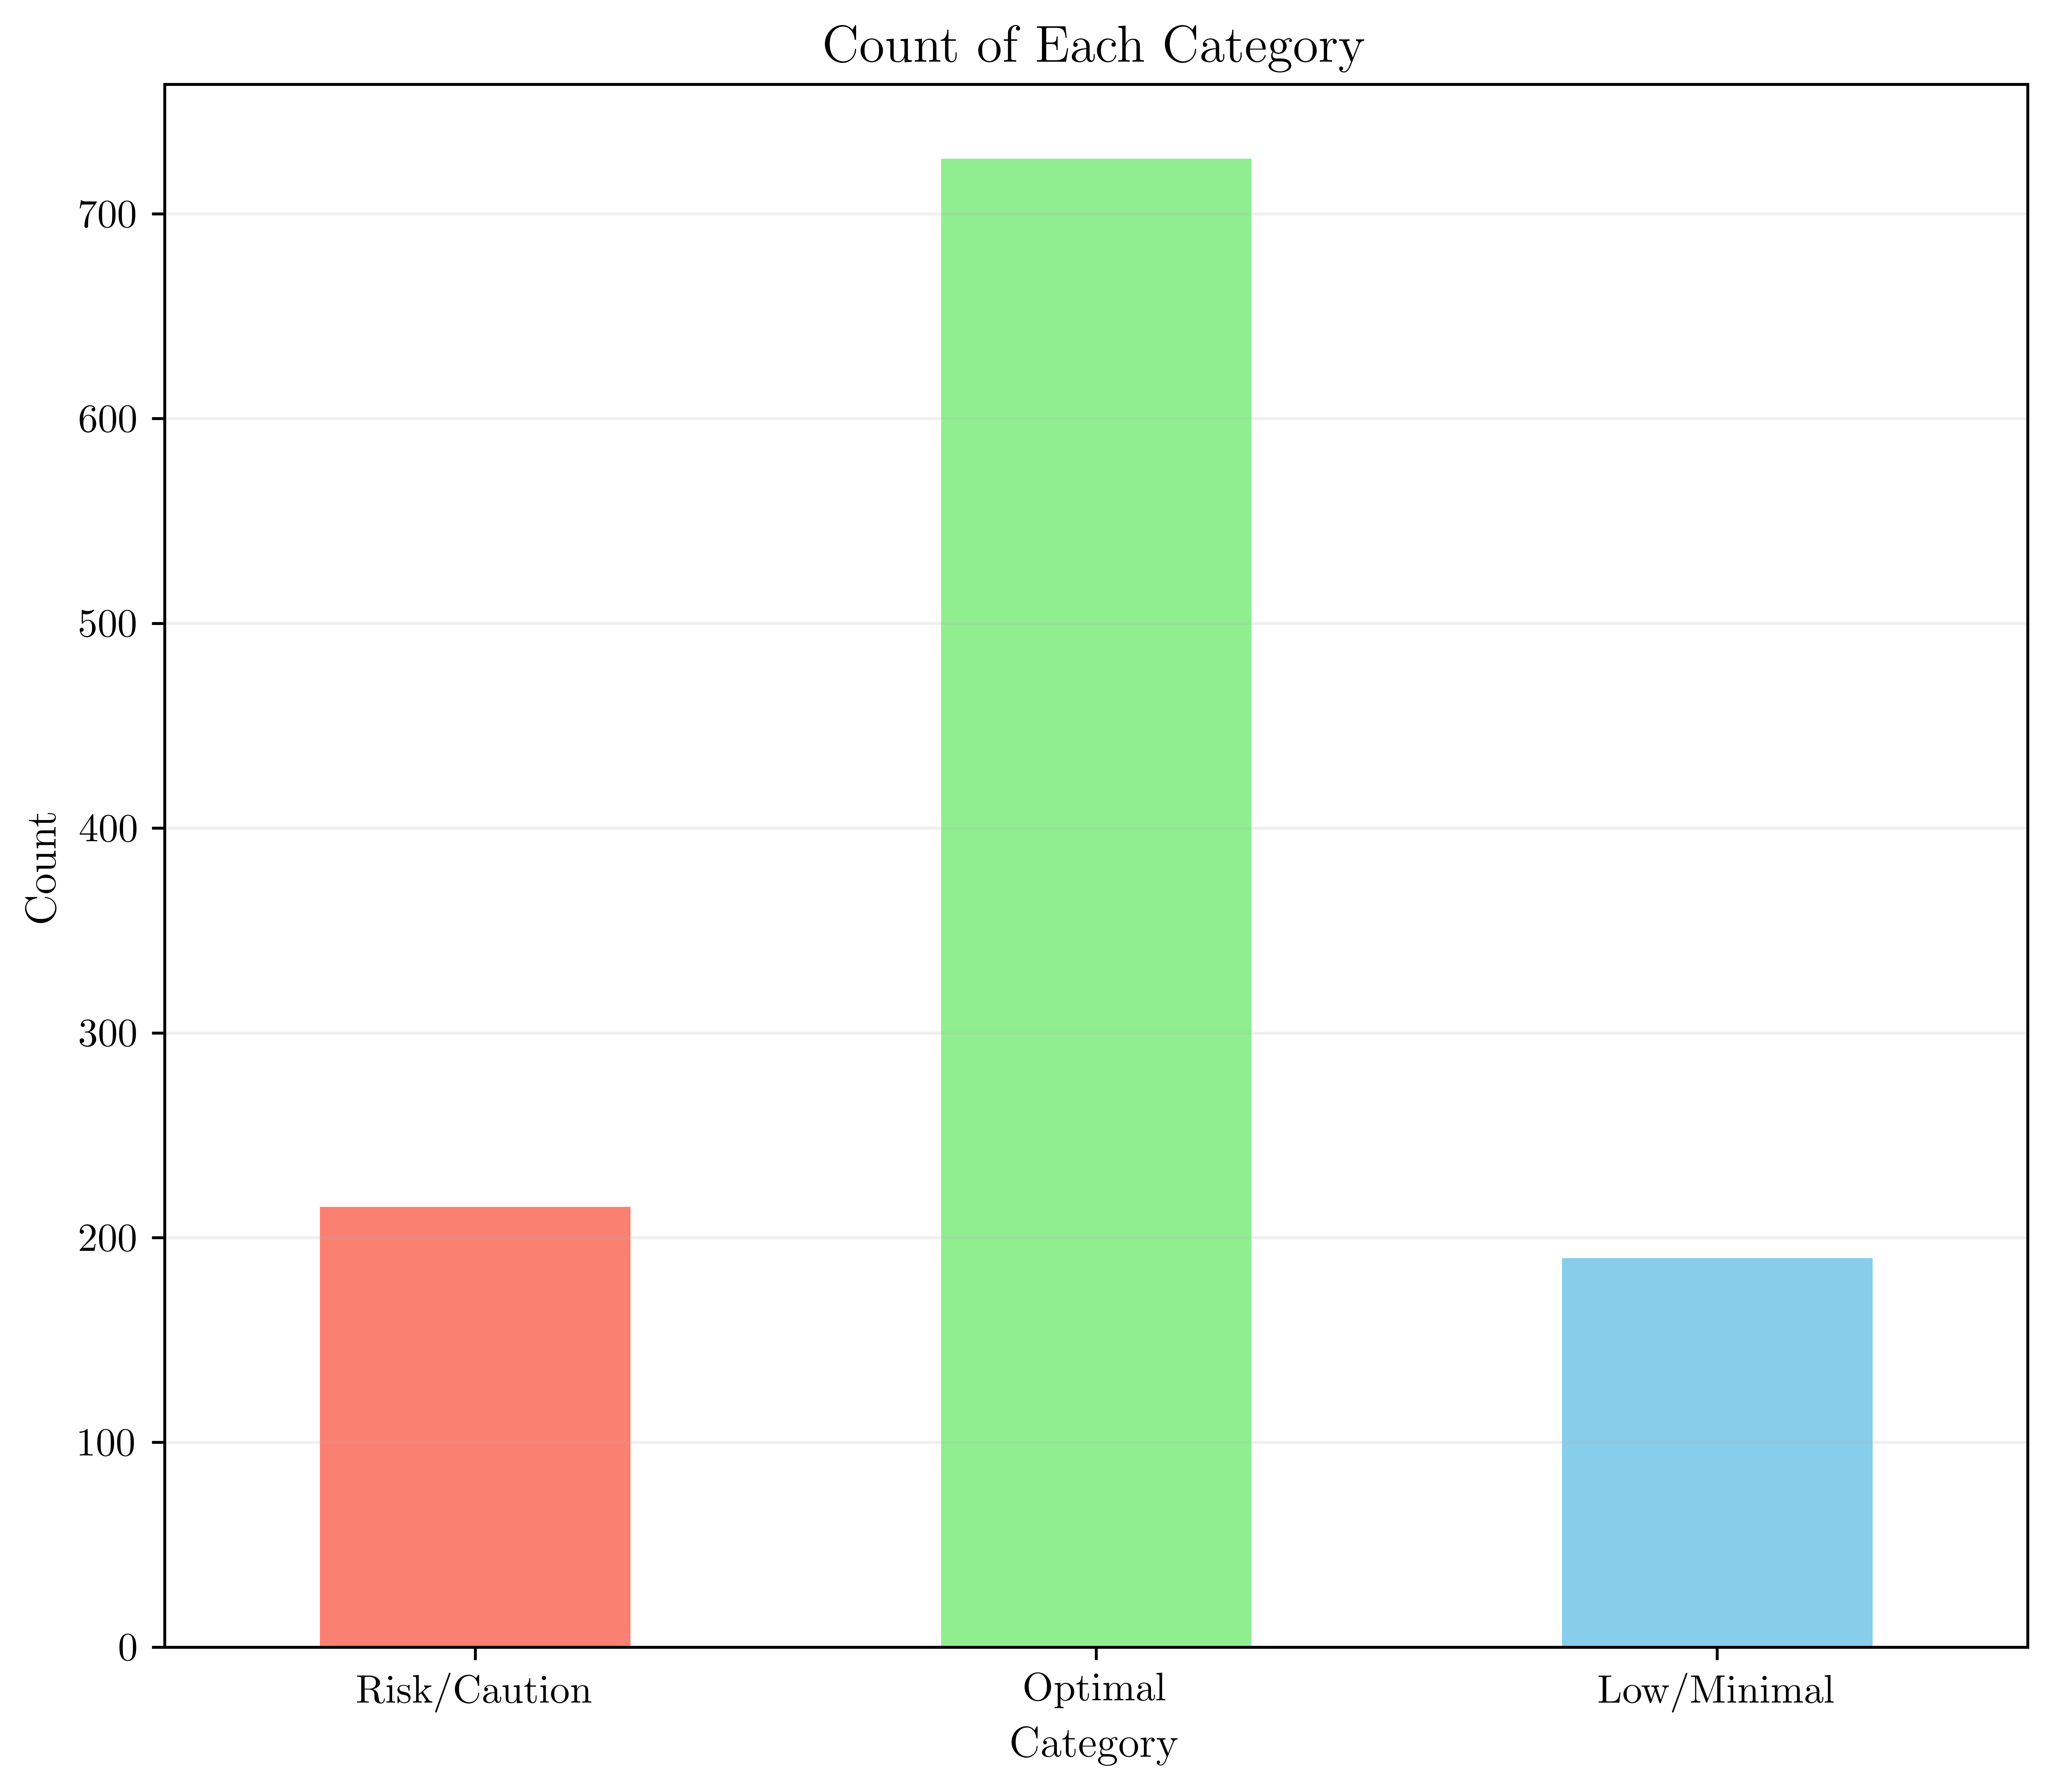
\includegraphics[width=1\linewidth]{assets/distribution_FatigInd(0).png}
    \caption{Bar plot of the new classes, once 'Caution' and 'Risk' are combined into one.}
    \label{histClasses}
\end{figure} %bar plot classes

At this stage, we opted to under sample our dataset to the number of observations of 'Risk/Caution', and over sample the observations in 'Low/Minimal', by imputing random samples from the pool of observations of 'Low/Minimal', ending up with 213 observations per class (regardless of gender). The use of SMOTE in this scenario would give continuous classes for our ordinal features, which wouldn't yield any physical meaning.

To assess how the different features vary among them and in relation to the target, we computed the correlation matrix as seen in Fig. \ref{fig:correlationMatrix}.

\begin{figure}[H]
    \centering
    \includegraphics[width=1\linewidth]{assets/correlation_matrix.png}
    \caption{Correlation matrix for all possible features considered for the models.}
    \label{fig:correlationMatrix}
\end{figure} % correlation matrix

From the correlation matrix it was possible to exclude several of the features, which was verified by how the classes are distributed across the scales for each feature. Fig. \ref{distpEffort} and \ref{distStSpirit} illustrate a proper and poor example of class distribution for the given features respectively.

Considering that the weights used in the coach's original estimation of fatigue were identical regardless of sex, the authors performed some simple models in order to decide if it would be necessary to split it. It could be verified that gender didn't have a significant impact in model performance, so we opted to use it as a feature. 

\begin{figure}[H]
    \centering
    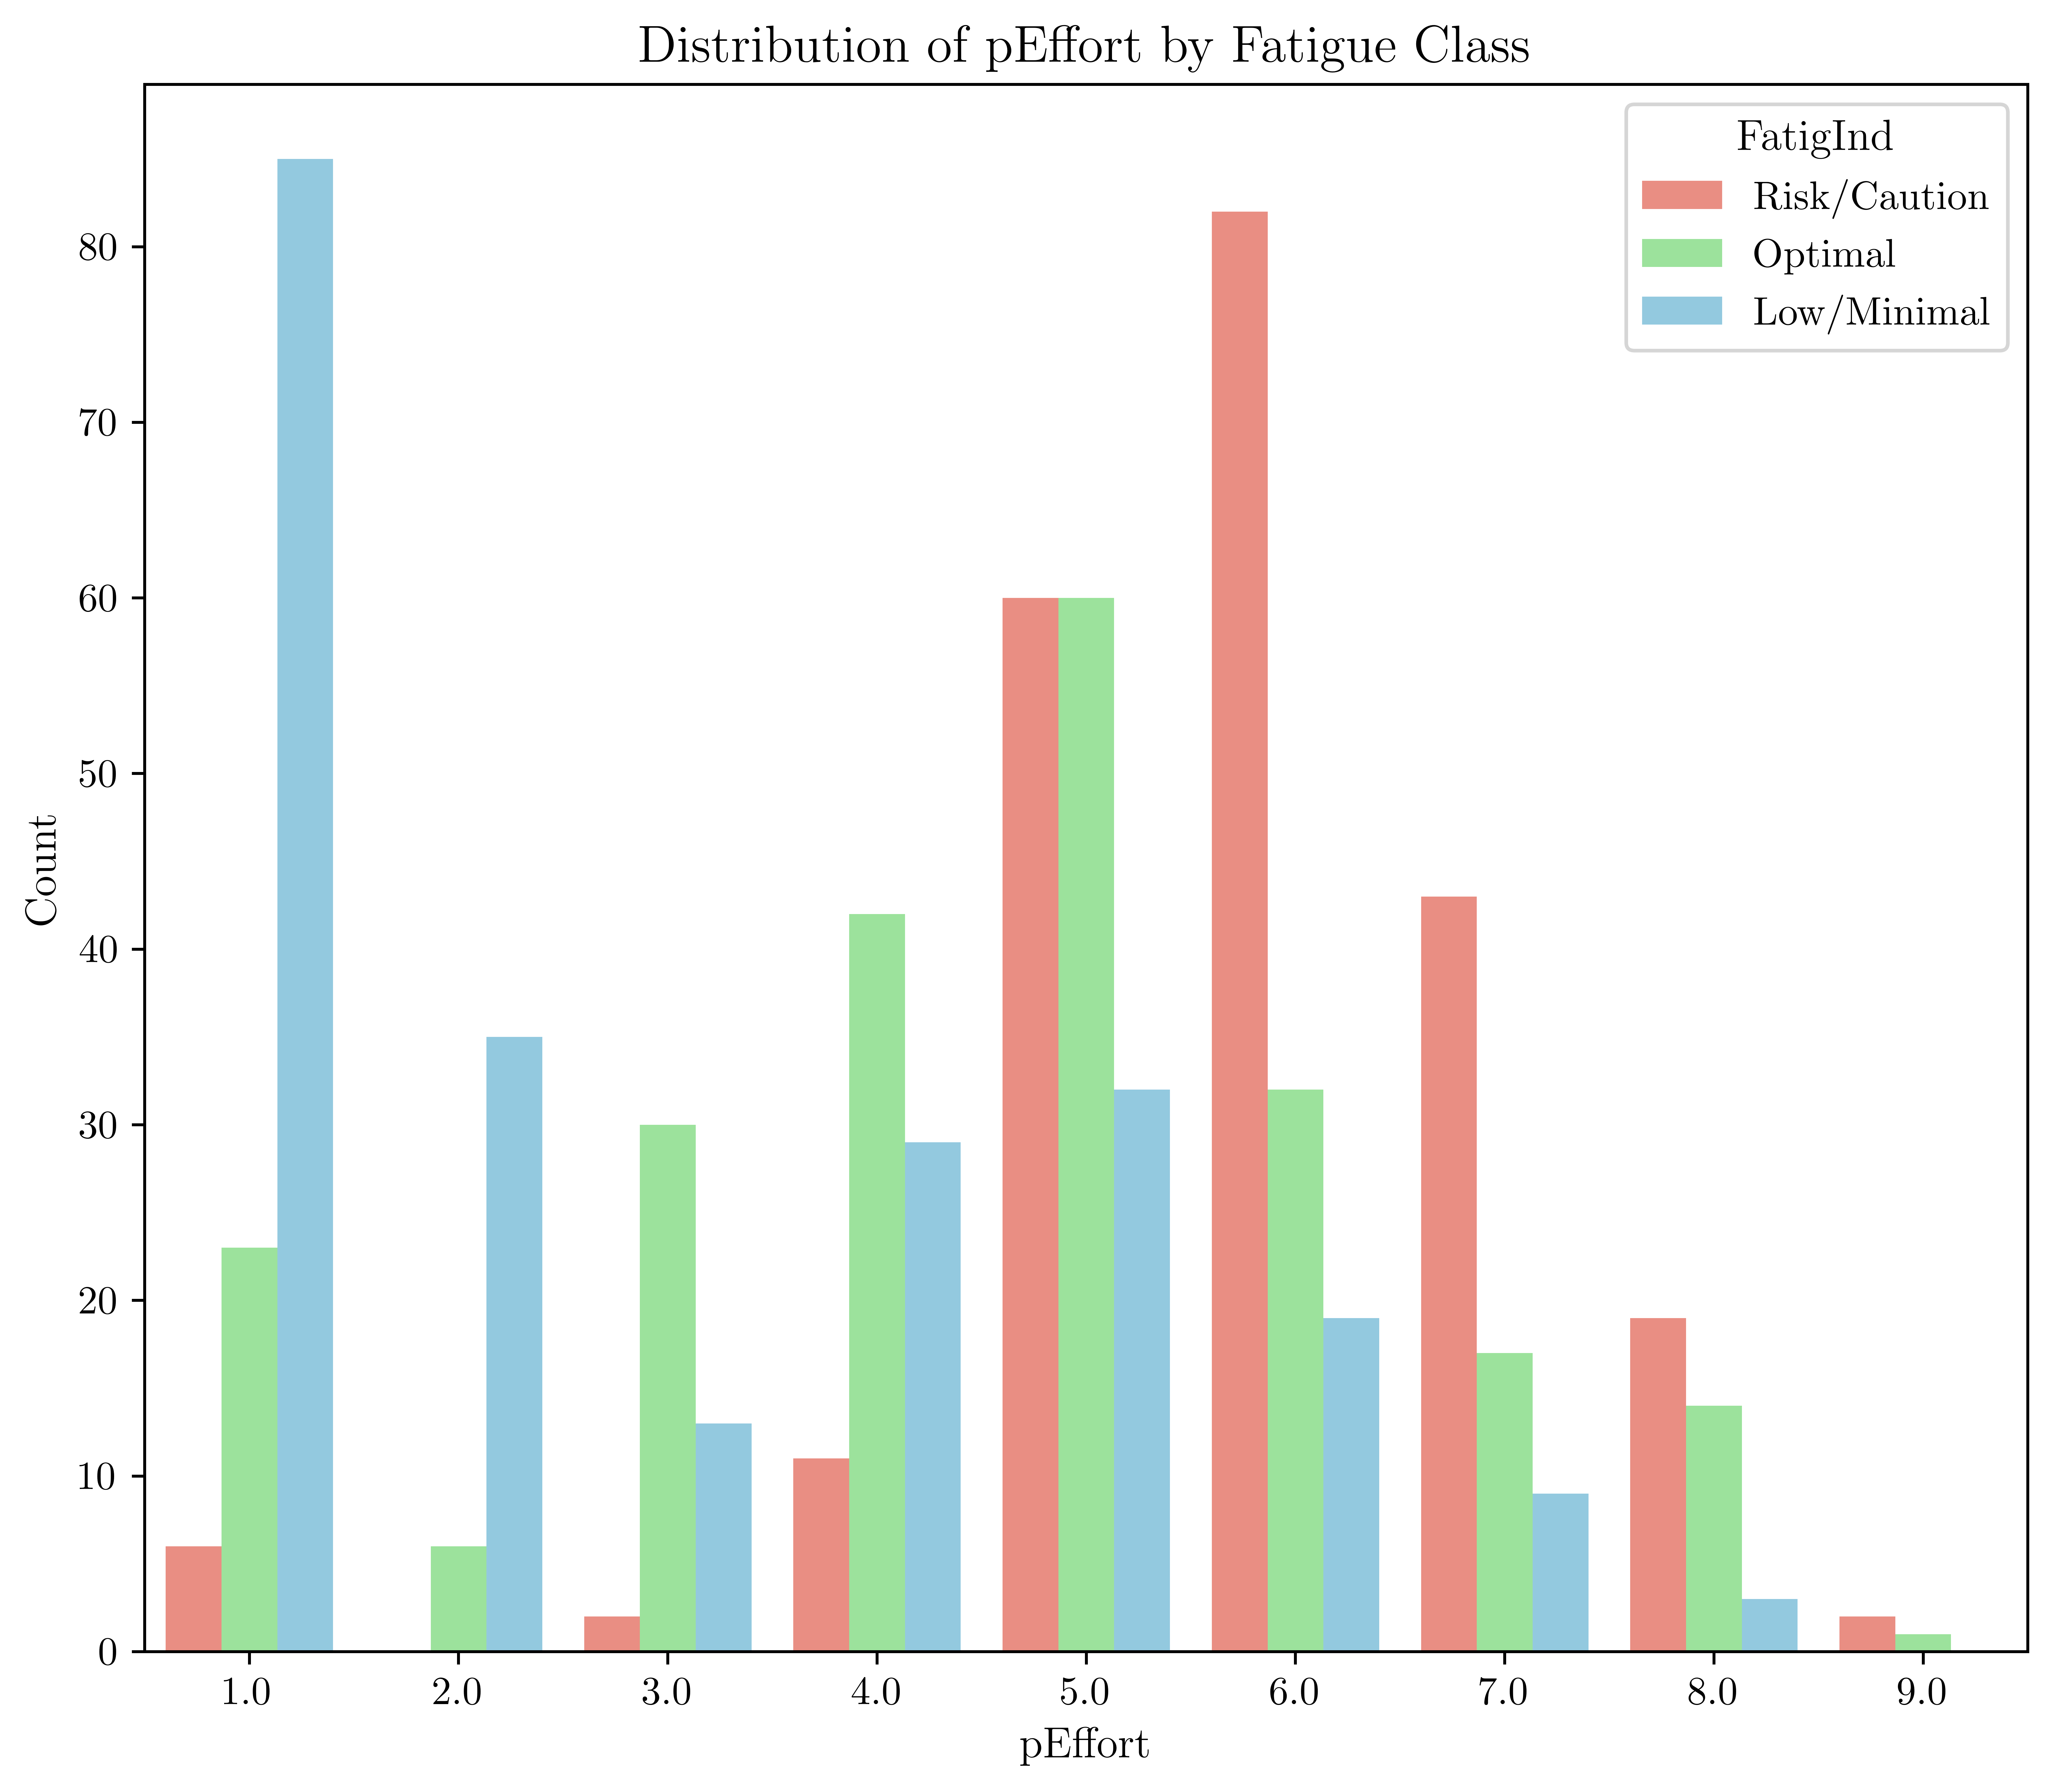
\includegraphics[width=1\linewidth]{assets/distribution_pEffort.png}
    \caption{Class distributions across perceived effort.}
    \label{distpEffort}
\end{figure} % not correlation matrix

\begin{figure}[H]
    \centering
    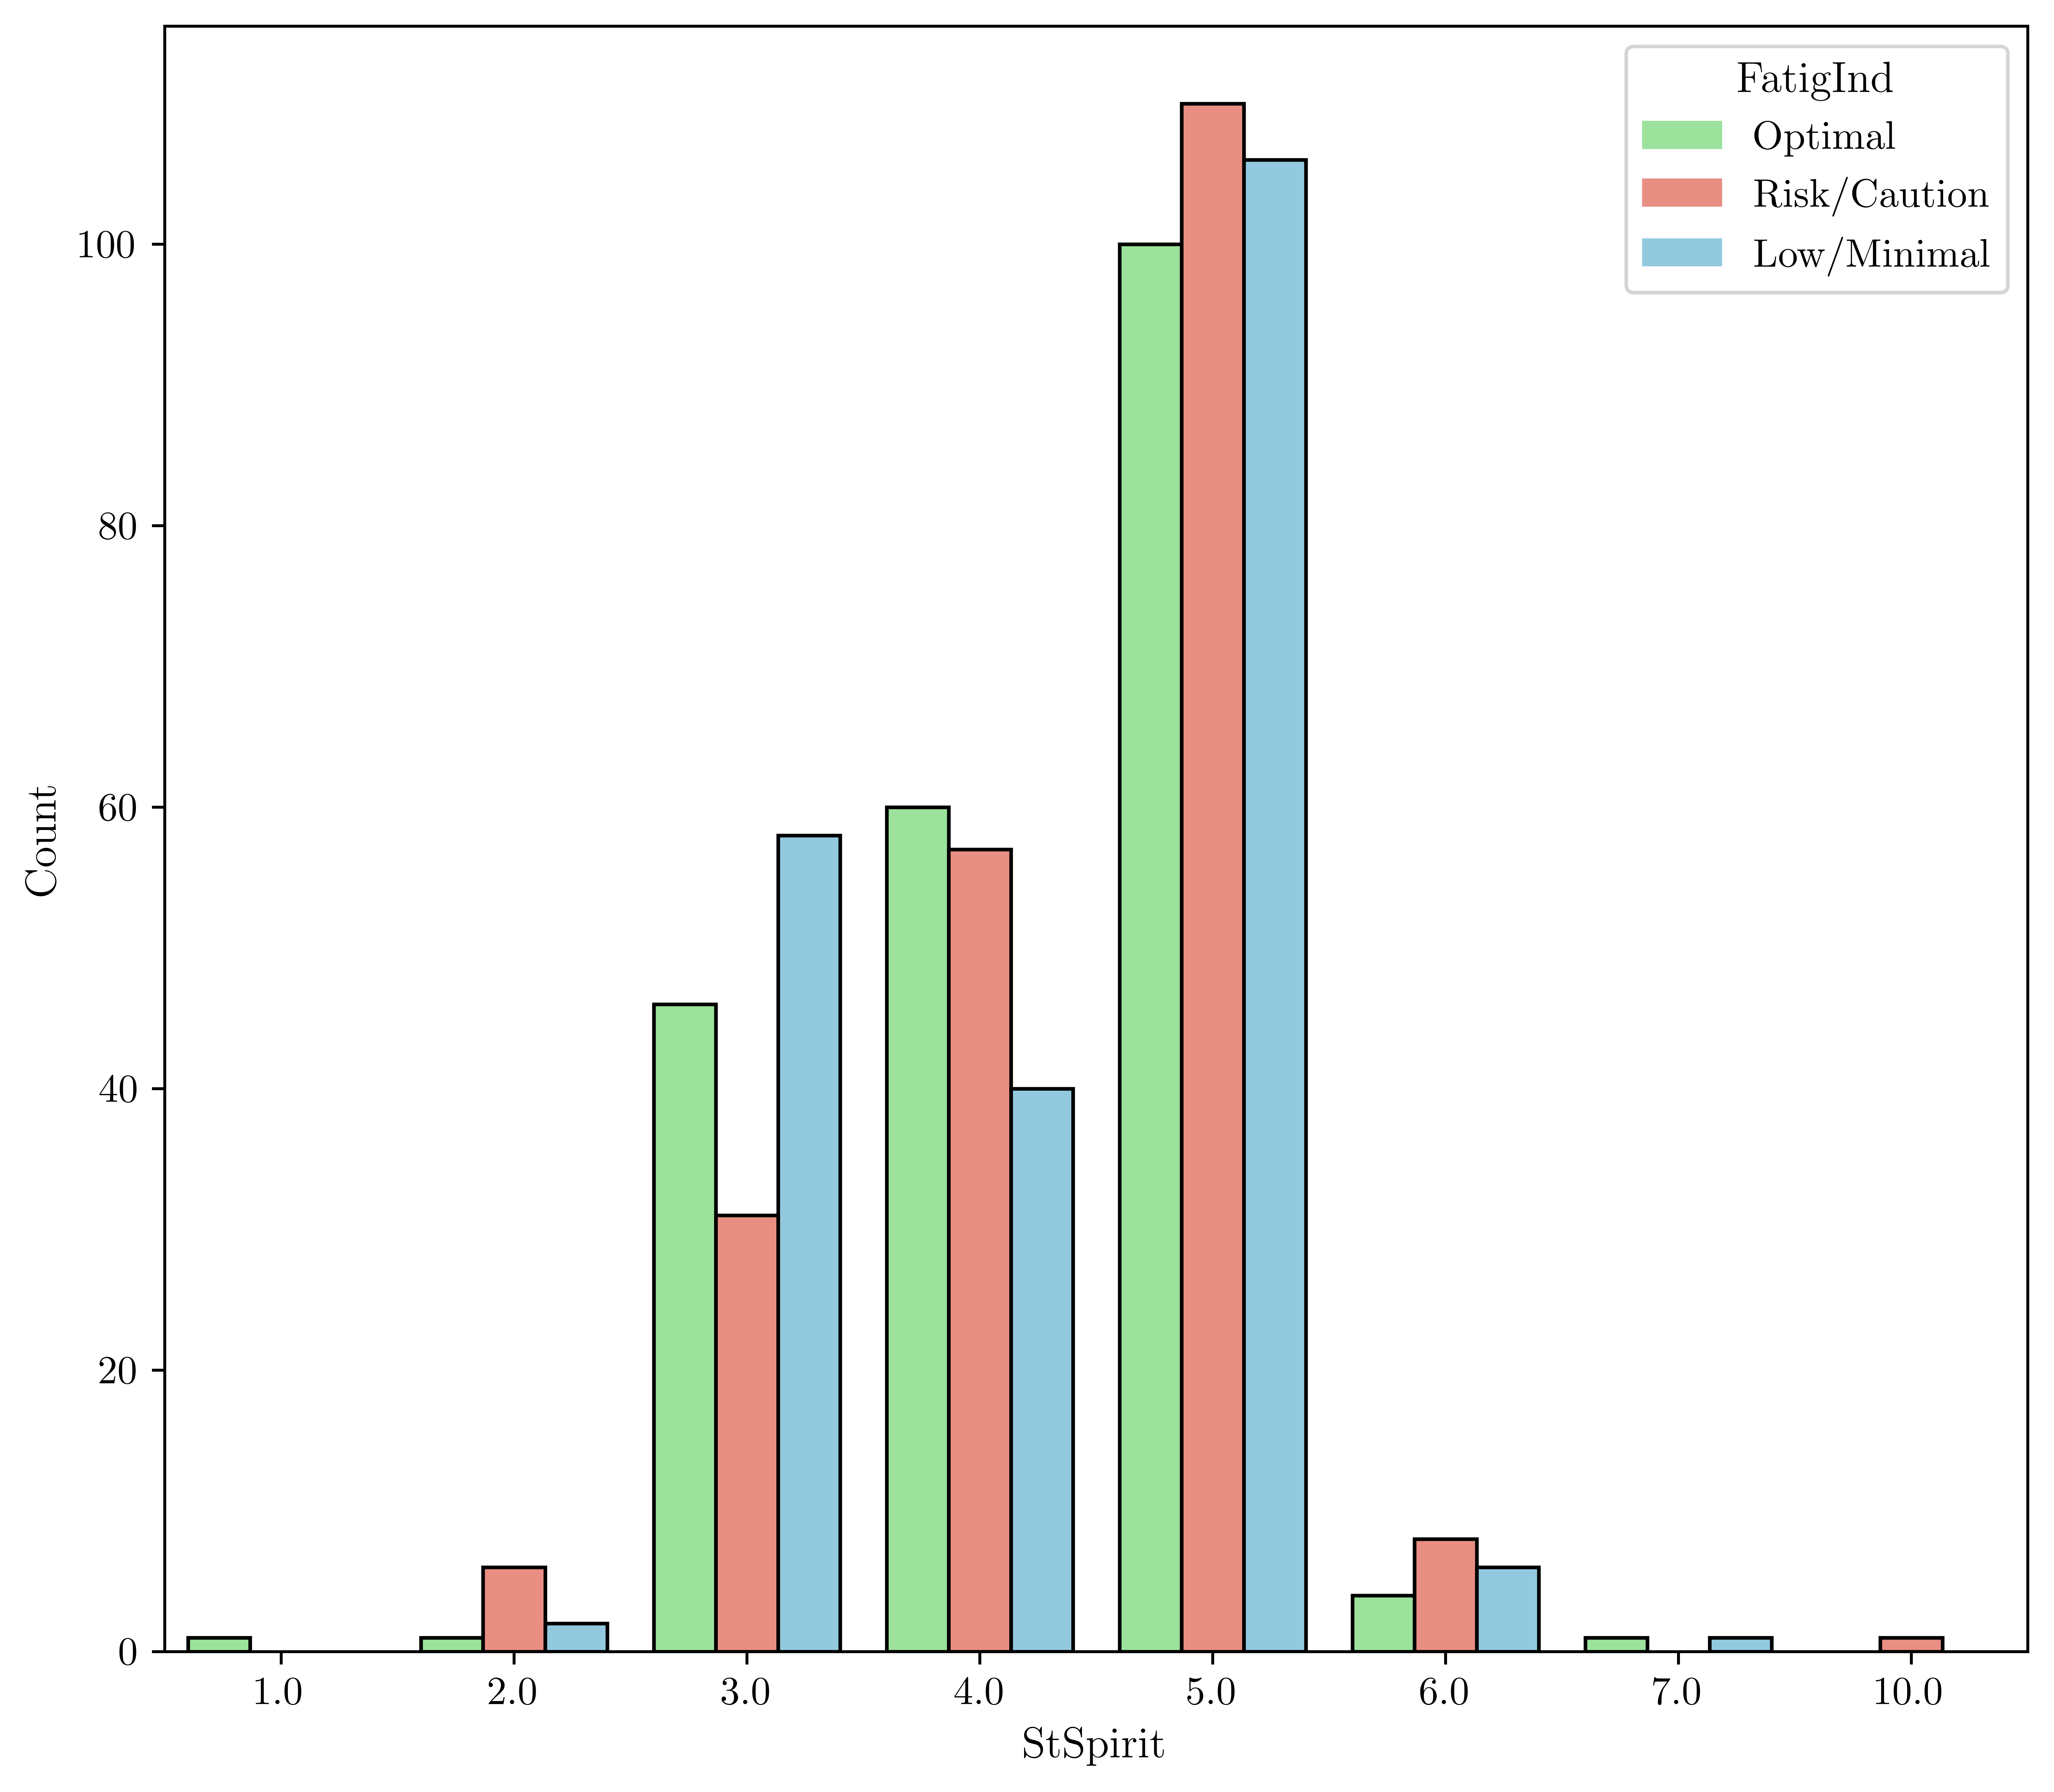
\includegraphics[width=1\linewidth]{assets/distribution_StSpirit.png}
    \caption{Class distributions across state spirit.}
    \label{distStSpirit}
\end{figure} % not correlation matrix


Fig. \ref{fadig_ts} illustrates the periodicity of higher training loads and subsequent lower intensity periods. It is important to refer that once the two higher intensity classes were combined the loss of granularity of how fatigue changes throughout the season is evident.  

\begin{figure}[H]
    \centering
    \begin{subfigure}[1]{\linewidth}
        \centering
        \includegraphics[width=0.91\linewidth]{assets/distribution_FatigInd(F_f).png}
        \caption{ }
        \label{fat_ff}
    \end{subfigure}
    
    \vspace{0.27cm}

    \begin{subfigure}[1]{\linewidth}
        \centering
        \includegraphics[width=0.91\linewidth]{assets/distribution_FatigInd(F_m).png}
        \caption{ }
        \label{fat_fm}
    \end{subfigure}
    
    \caption{Daily fatigue trends for athletes (a) F\_f and (b) F\_m.}
    \label{fadig_ts}
\end{figure} %precision, recall, f1


In order to keep the time series nature of training, increase and decrease of training intensity, and varying fatigue with training, a exponentially weighted moving averages (EWMA) was included \cite{Williams17}.

This way memory is introduced in the models, allowing consideration of the decay in the weights of events further away from any given day. The mathematical expression used to calculate EWMA for each selected feature is,
\begin{equation*}
    \text{EWMA}_{\text{today}} = \text{Feature}_{\text{today}} \cdot \lambda_a + (1 - \lambda_a) \cdot \text{EWMA}_{\text{yesterday}}
\end{equation*}
where $\lambda_a$ is a value between 0 and 1 that represents the degree of decay, with higher values discounting older observations at a faster rate. The $\lambda_a$ is given by:
\begin{equation*}
    \lambda_a = \frac{2}{N + 1}
\end{equation*} 

Where $N$ is the time decay constant, with a 1 week and 4 week workload representing the acute and chronic workloads, respectively \cite{Murray16}.

At this point, it was possible to select the most relevant features for the ML models, which are shown in Table \ref{features_selection}.

\begin{table}[H]
\centering
\caption{Feature descriptions}
\label{features_selection}
\begin{tabular}{ll}
\toprule
\textbf{Feature} & \textbf{Description} \\
\midrule
\textit{Sex\_F} & Athlete's gender.  \\
\textit{pEffort} & Perceived effort from the workout. \\
\textit{uaI} & Intensity from each workout. \\
\textit{SleepInd} & Index based on quality of sleep and time in bed. \\
\textit{Appetite(MA6)} & Appetite measure, averaged with EWMA(6). \\
\textit{pEffort(MA6)} & \textit{pEffort} averaged with EWMA(6). \\
\textit{uaI(MA6)} & \textit{uaI} averaged with EWMA(6). \\
\textit{SleepInd(MA6)} & \textit{SleepInd} averaged with EWMA(6). \\
\bottomrule
\end{tabular}
\end{table}


\section{Classification Models}

In the following sections, \ref{logreg_section} to \ref{dtree_section}, the results for the three machine learning models are presented and detailed in equal fashion, to ease the discussion and interpretation in the section \ref{discussion_sec}. As was mentioned in the methodology, the modeling approach was the same for all, and here the training dataset results are presented first, followed by the test dataset results.

\section{Logistic Regression} \label{logreg_section}

The logistic regression model was developed by exploring different ranges for the hyperparameters, including $C$, the inverse of the regularization parameter, and allowing for the selection of various regularization methods, as can be assessed in Table \ref{parametrosLogReg}.

\begin{table}[H]
\centering
\caption{Logistic regression model hyperparameters search space.}
\label{parametrosLogReg}
\begin{tabular}{ll}
\toprule
\textbf{Hyperparameter} & \textbf{Possible Values} \\
\midrule
$C$ & $[0.01, 300]$ \\ 
Regularization & \{$L1$, $L2$, none\} \\
\bottomrule
\end{tabular}
\end{table} %hyperparameters

Due to the suboptimal performance of the 'Optimal' class in terms of precision, it was also decided to adjust the class weights for 'Risk/Caution' and 'Low/Minimal' within a range of 0.1 to 2. The resulting model with the highest accuracy is illustrated in Fig.~\ref{logregWt}.

\begin{figure}[H]
    \centering
    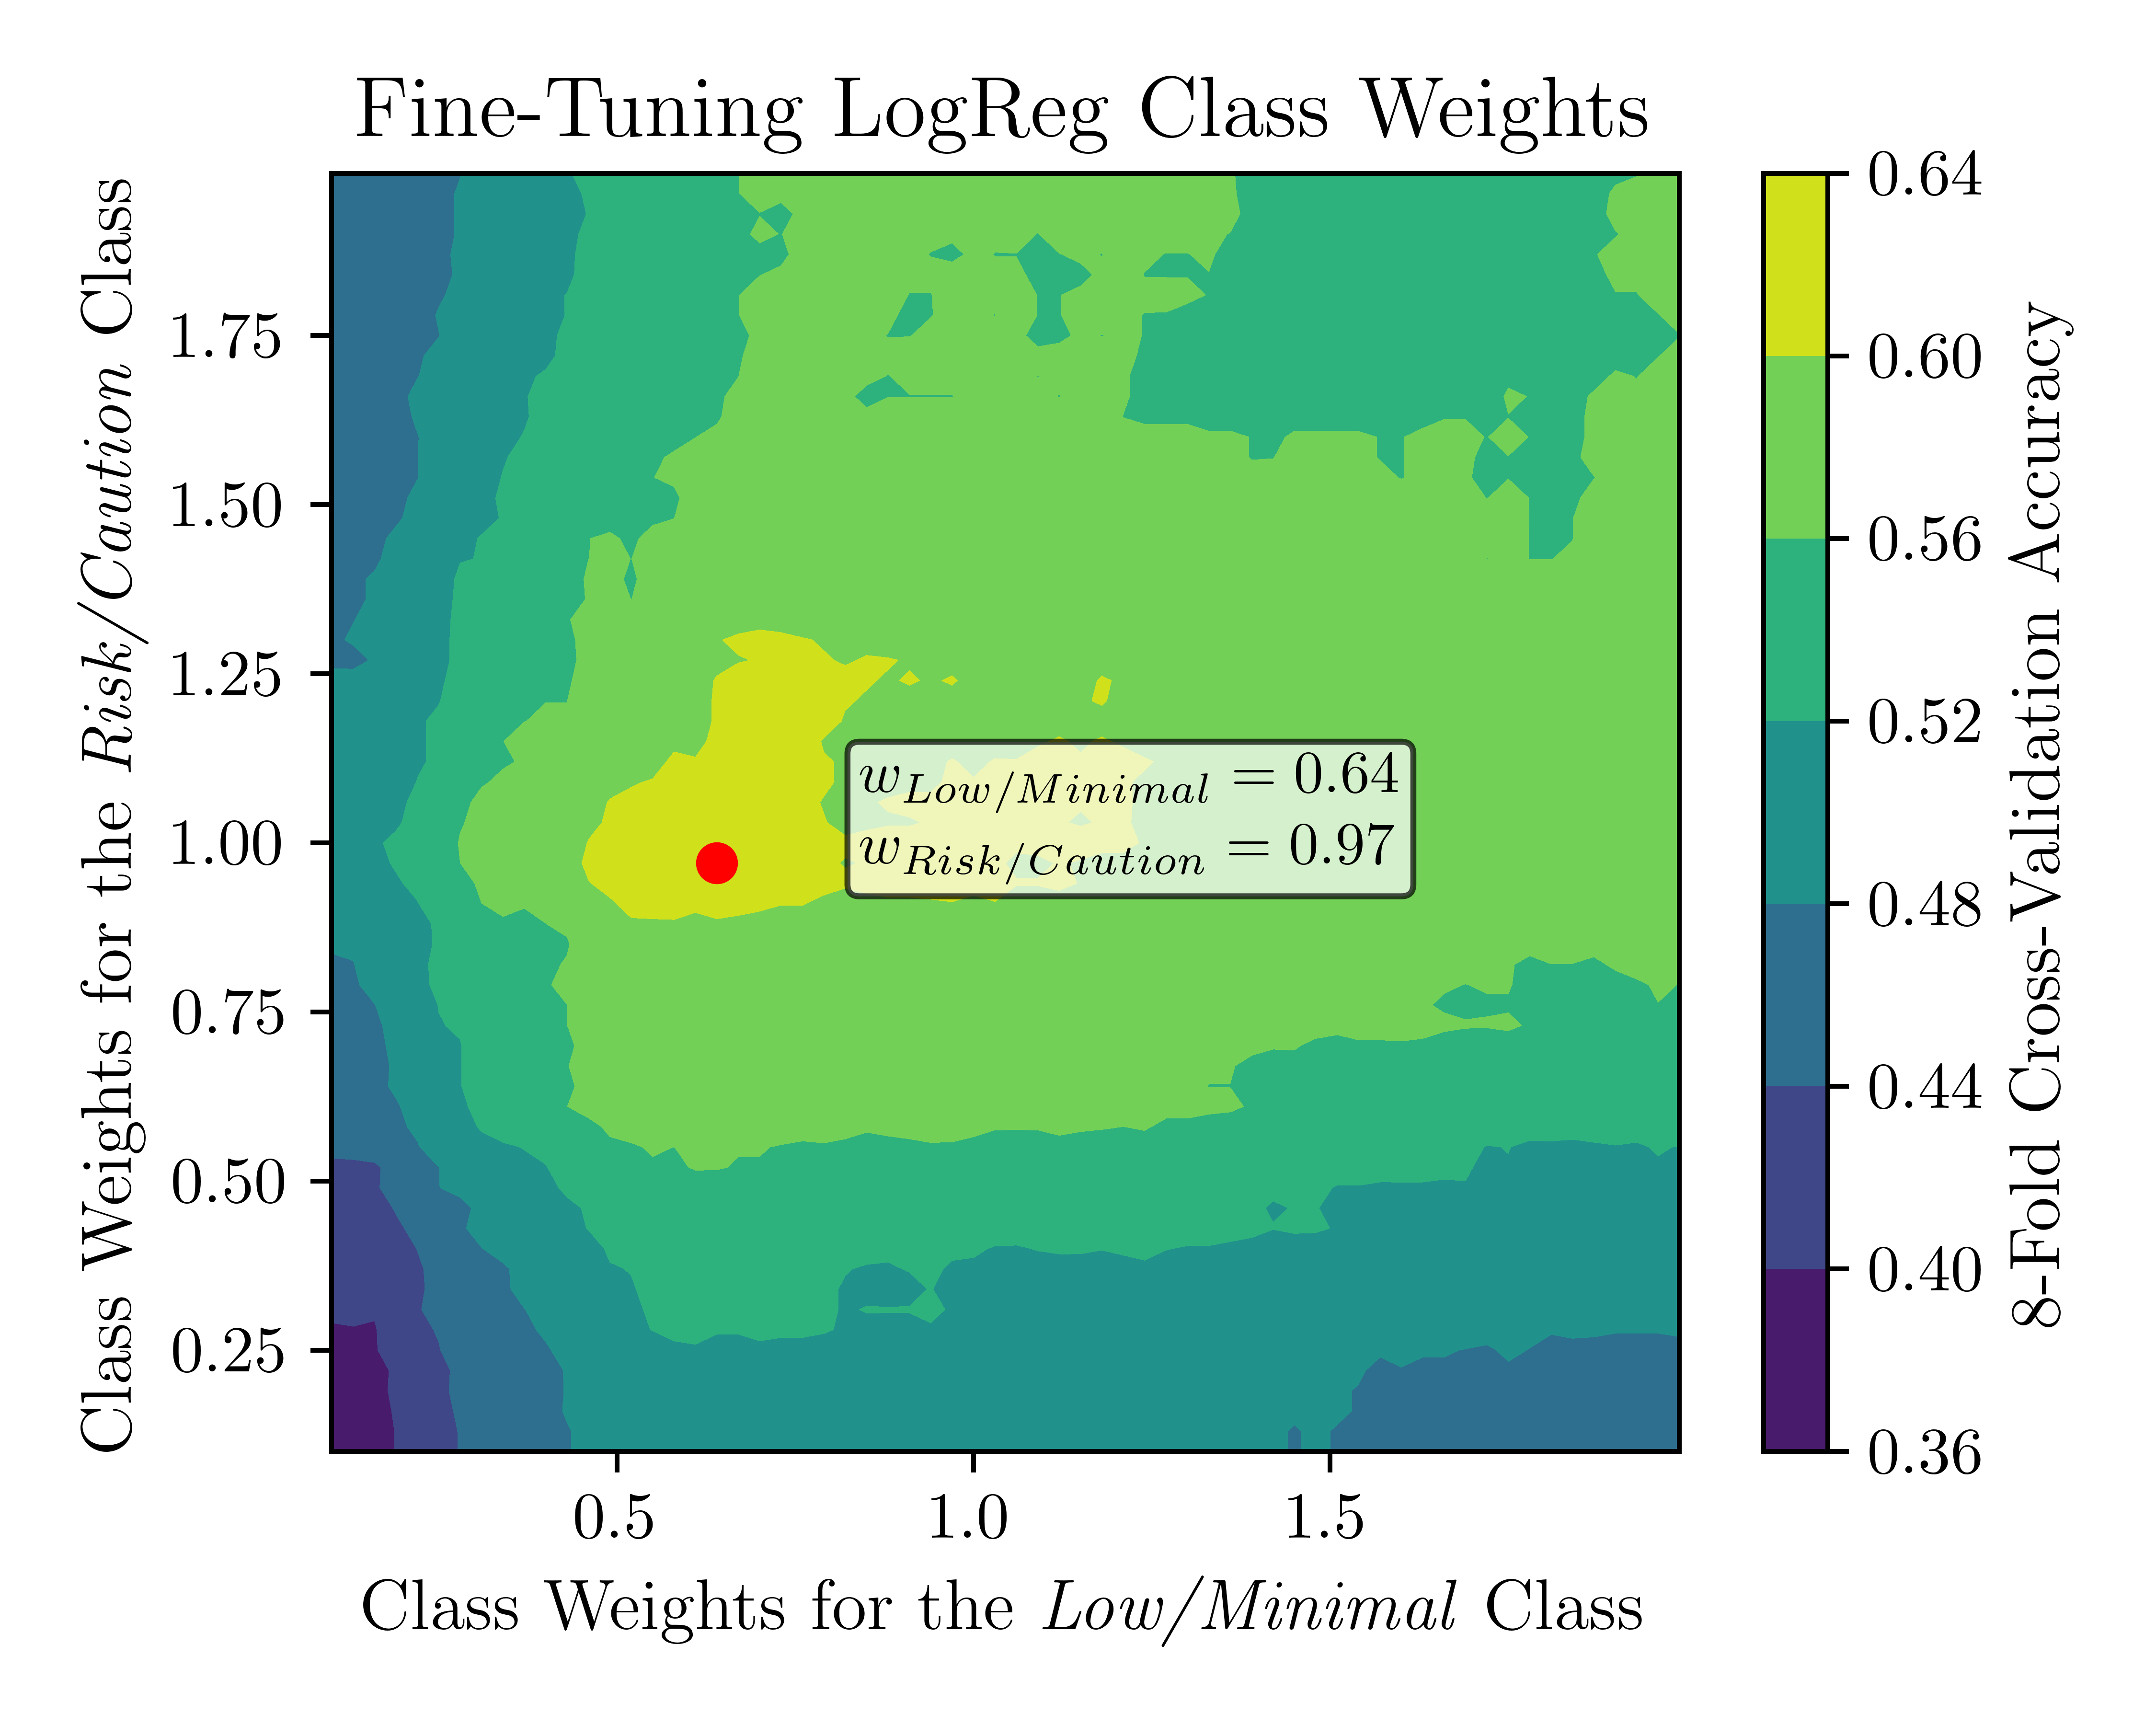
\includegraphics[width=.9\linewidth]{assets/LOGR_class_weights.png}
    \caption{Effect of the 'Risk/Caution' and 'Low/Minimal' classes weight on LogReg model accuracy.}
    \label{logregWt}
\end{figure} %class weights

Since the highest accuracy was achieved with class weights of 0.64 for 'Low/Minimal' and 0.97 for 'Risk/Caution', these values were selected, while the original weight for the 'Optimal' class was retained ($w_{optimal} = 1$). For model optimization, the remaining hyperparameters were set to $C \approx 2.13$, the cost function was $L1$ (Lasso regularization) and the solver used was SAGA (Stochastic Average Gradient Augmented). Despite the fact that it is most commonly used for large datasets, it was the best performing kernel of those available in the initial assessment, with the advantage that it allowed for regularization. The equation for the solver is given by,
\begin{equation*}
\underset{\theta}{\text{min}} \, \frac{1}{N} \sum_{i=1}^{N} \log\left(1 + \exp\left(-y_i \theta^\top x_i\right)\right) + \frac{1}{C} R(\theta)
\end{equation*} % SAGA solver

The learning curve shown in Fig. \ref{lcLogReg} illustrates the relationship between the training set size and the performance of the adjusted model, providing valuable insight to assess the model's behavior in terms of overfitting or underfitting. In this case, the learning curves from the training and the cross-validation converge after the largest training set size of 450, with no signs of overfitting.

\begin{figure}[H]
    \centering
    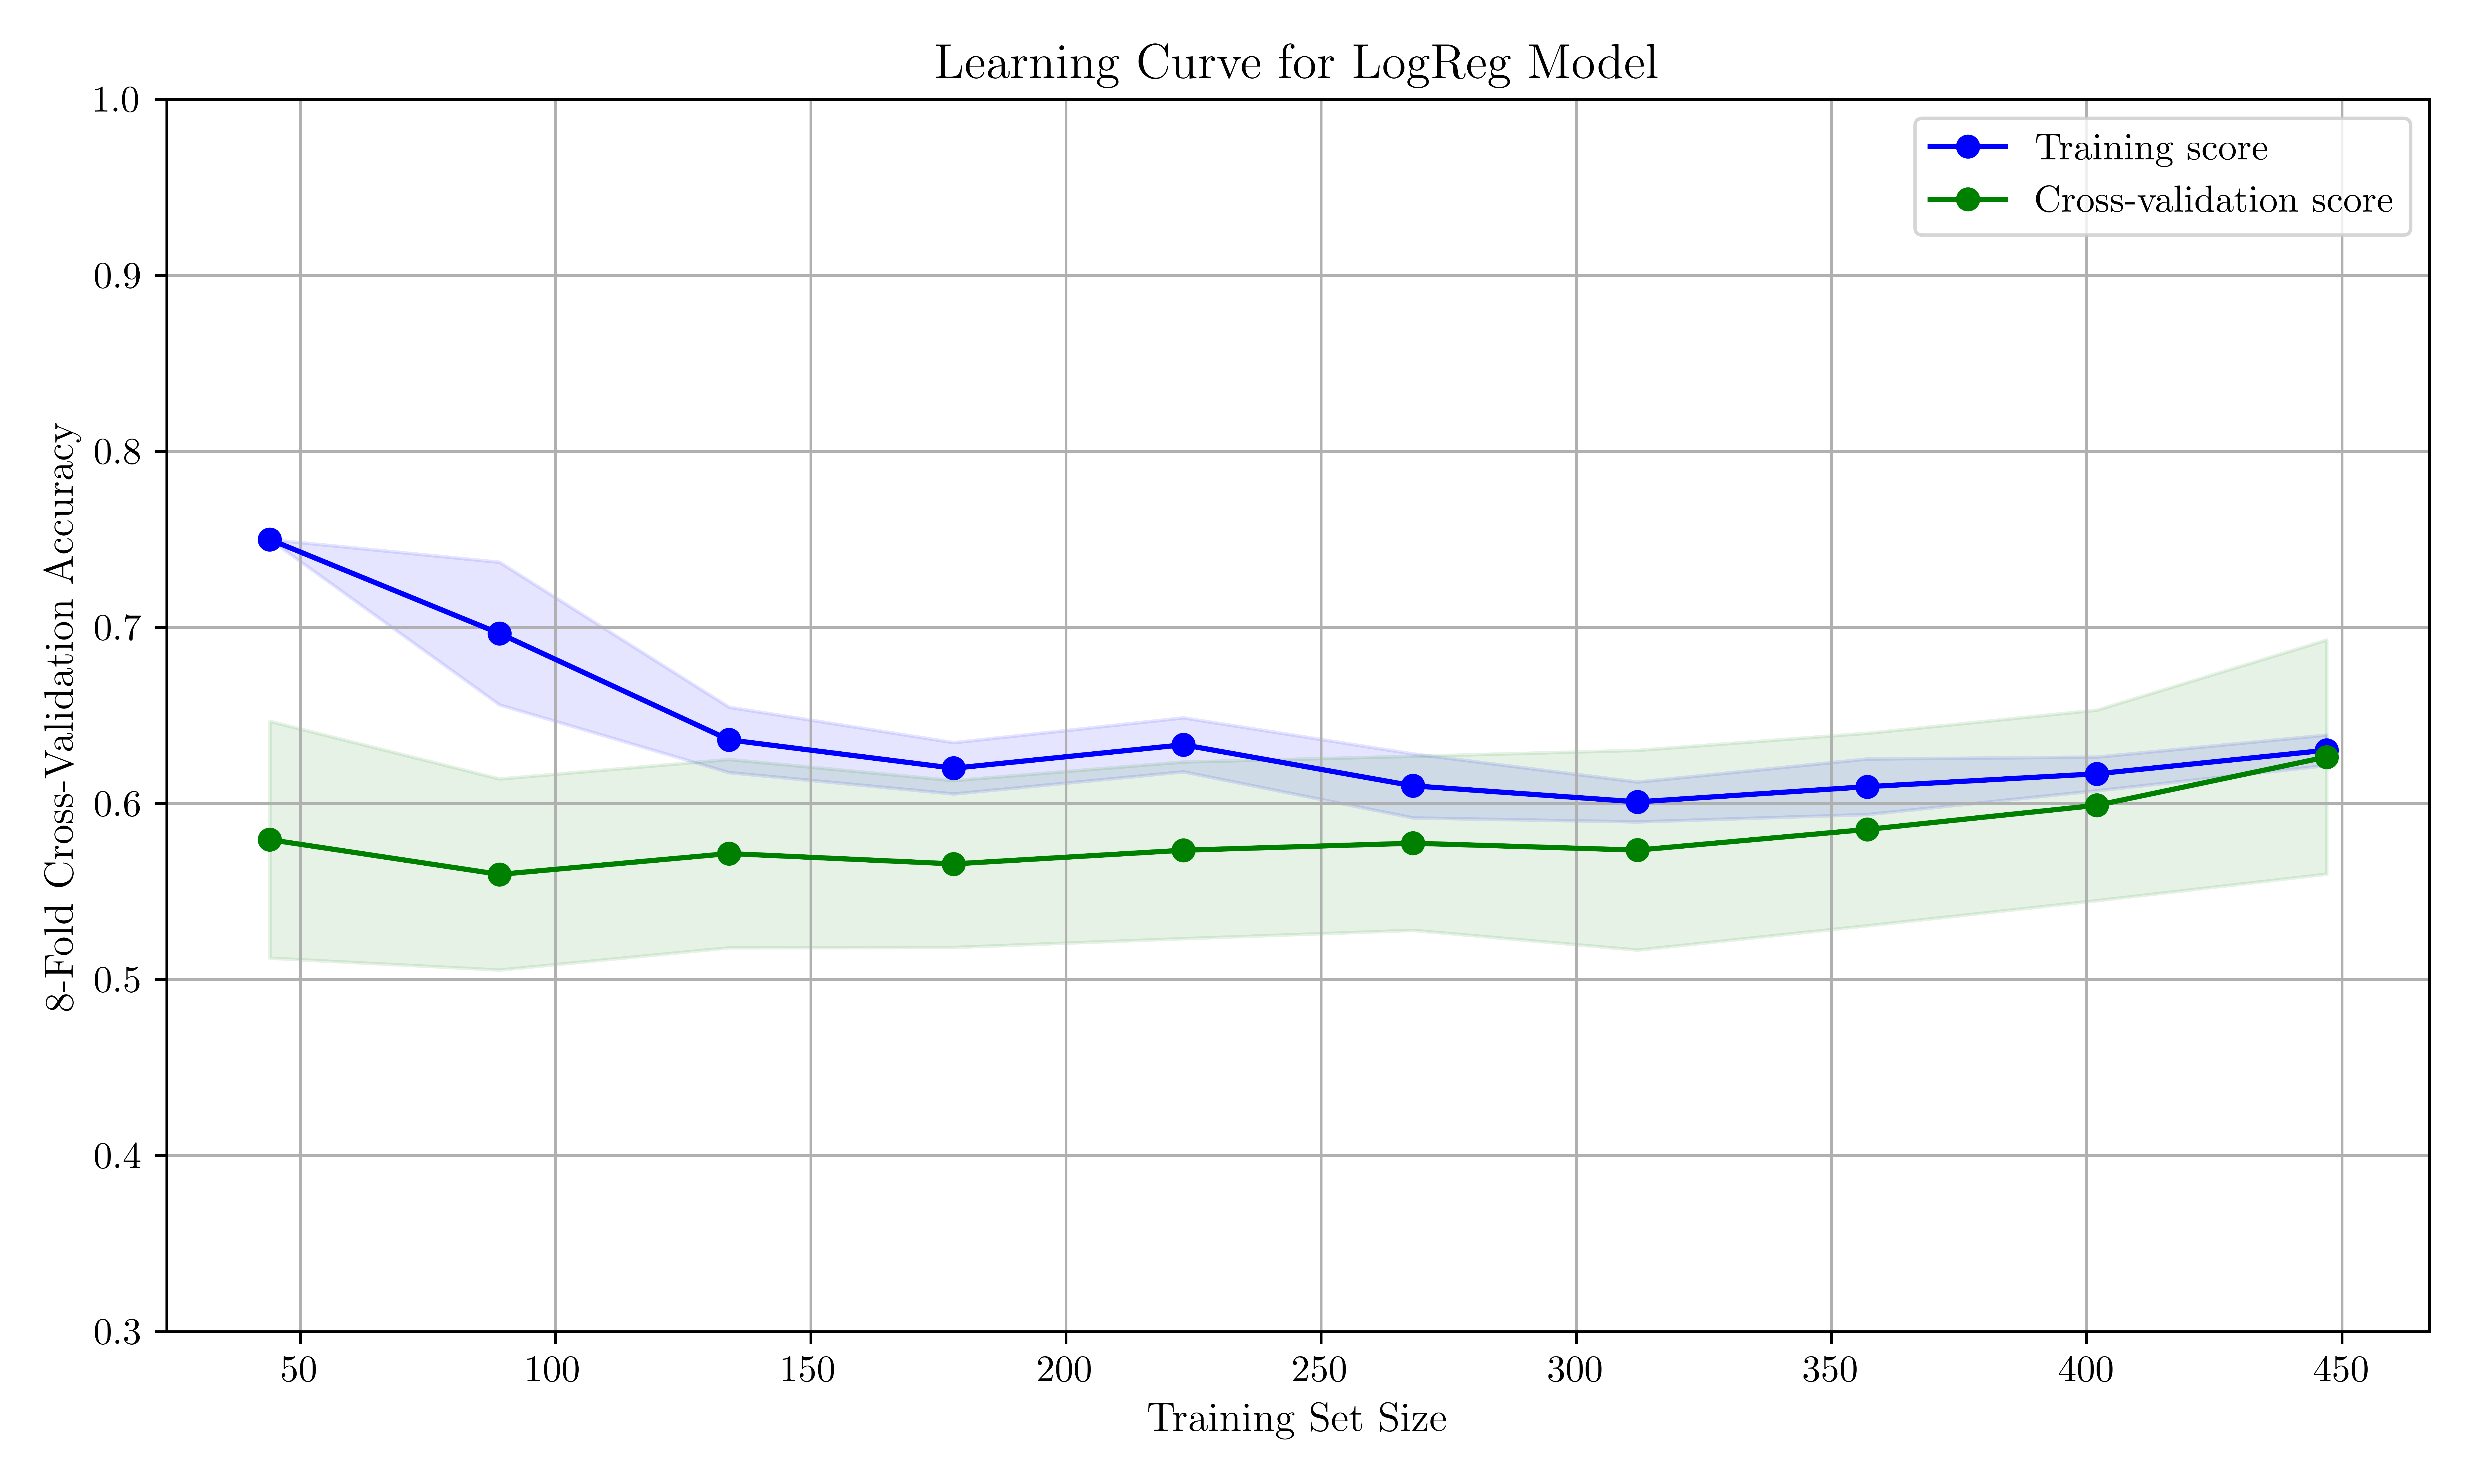
\includegraphics[width=1\linewidth]{assets/LOGR_lercurve.png}
    \caption{LogReg model performance using learning curve representation across varying training data sizes.}
    \label{lcLogReg}
\end{figure} %lc 

Considering the confusion matrices of the training (Fig.~\ref{cf_train_LogReg}) and test datasets (Fig.~\ref{cm_Test_LogReg}), it is possible to learn how well the model attributes true and false positives, and how they are distributed. For this particular model it is visible how similar they are, and how much better the prediction performance is for the classes in the extremities ('Low/Minimal' and 'Risk/Caution'), regardless of the weight attributed to the 'Optimal' class (even though a marginal improvement was observed compared to the initial weightless model).

The classification report provides a more straight forward comparison between the training (Table~\ref{crTrainLogReg}) and the test datasets (Table~\ref{crTestLogREg}), while showing class specific the performance metrics, further confirming the interpretation of the confusion matrix. Both classification reports present similar values, which is a good indicator that the model is properly fitted. As previously mentioned, the performance metrics are worse for 'Optimal' when compared to the remaining classes.

\begin{figure}[H]
    \centering
    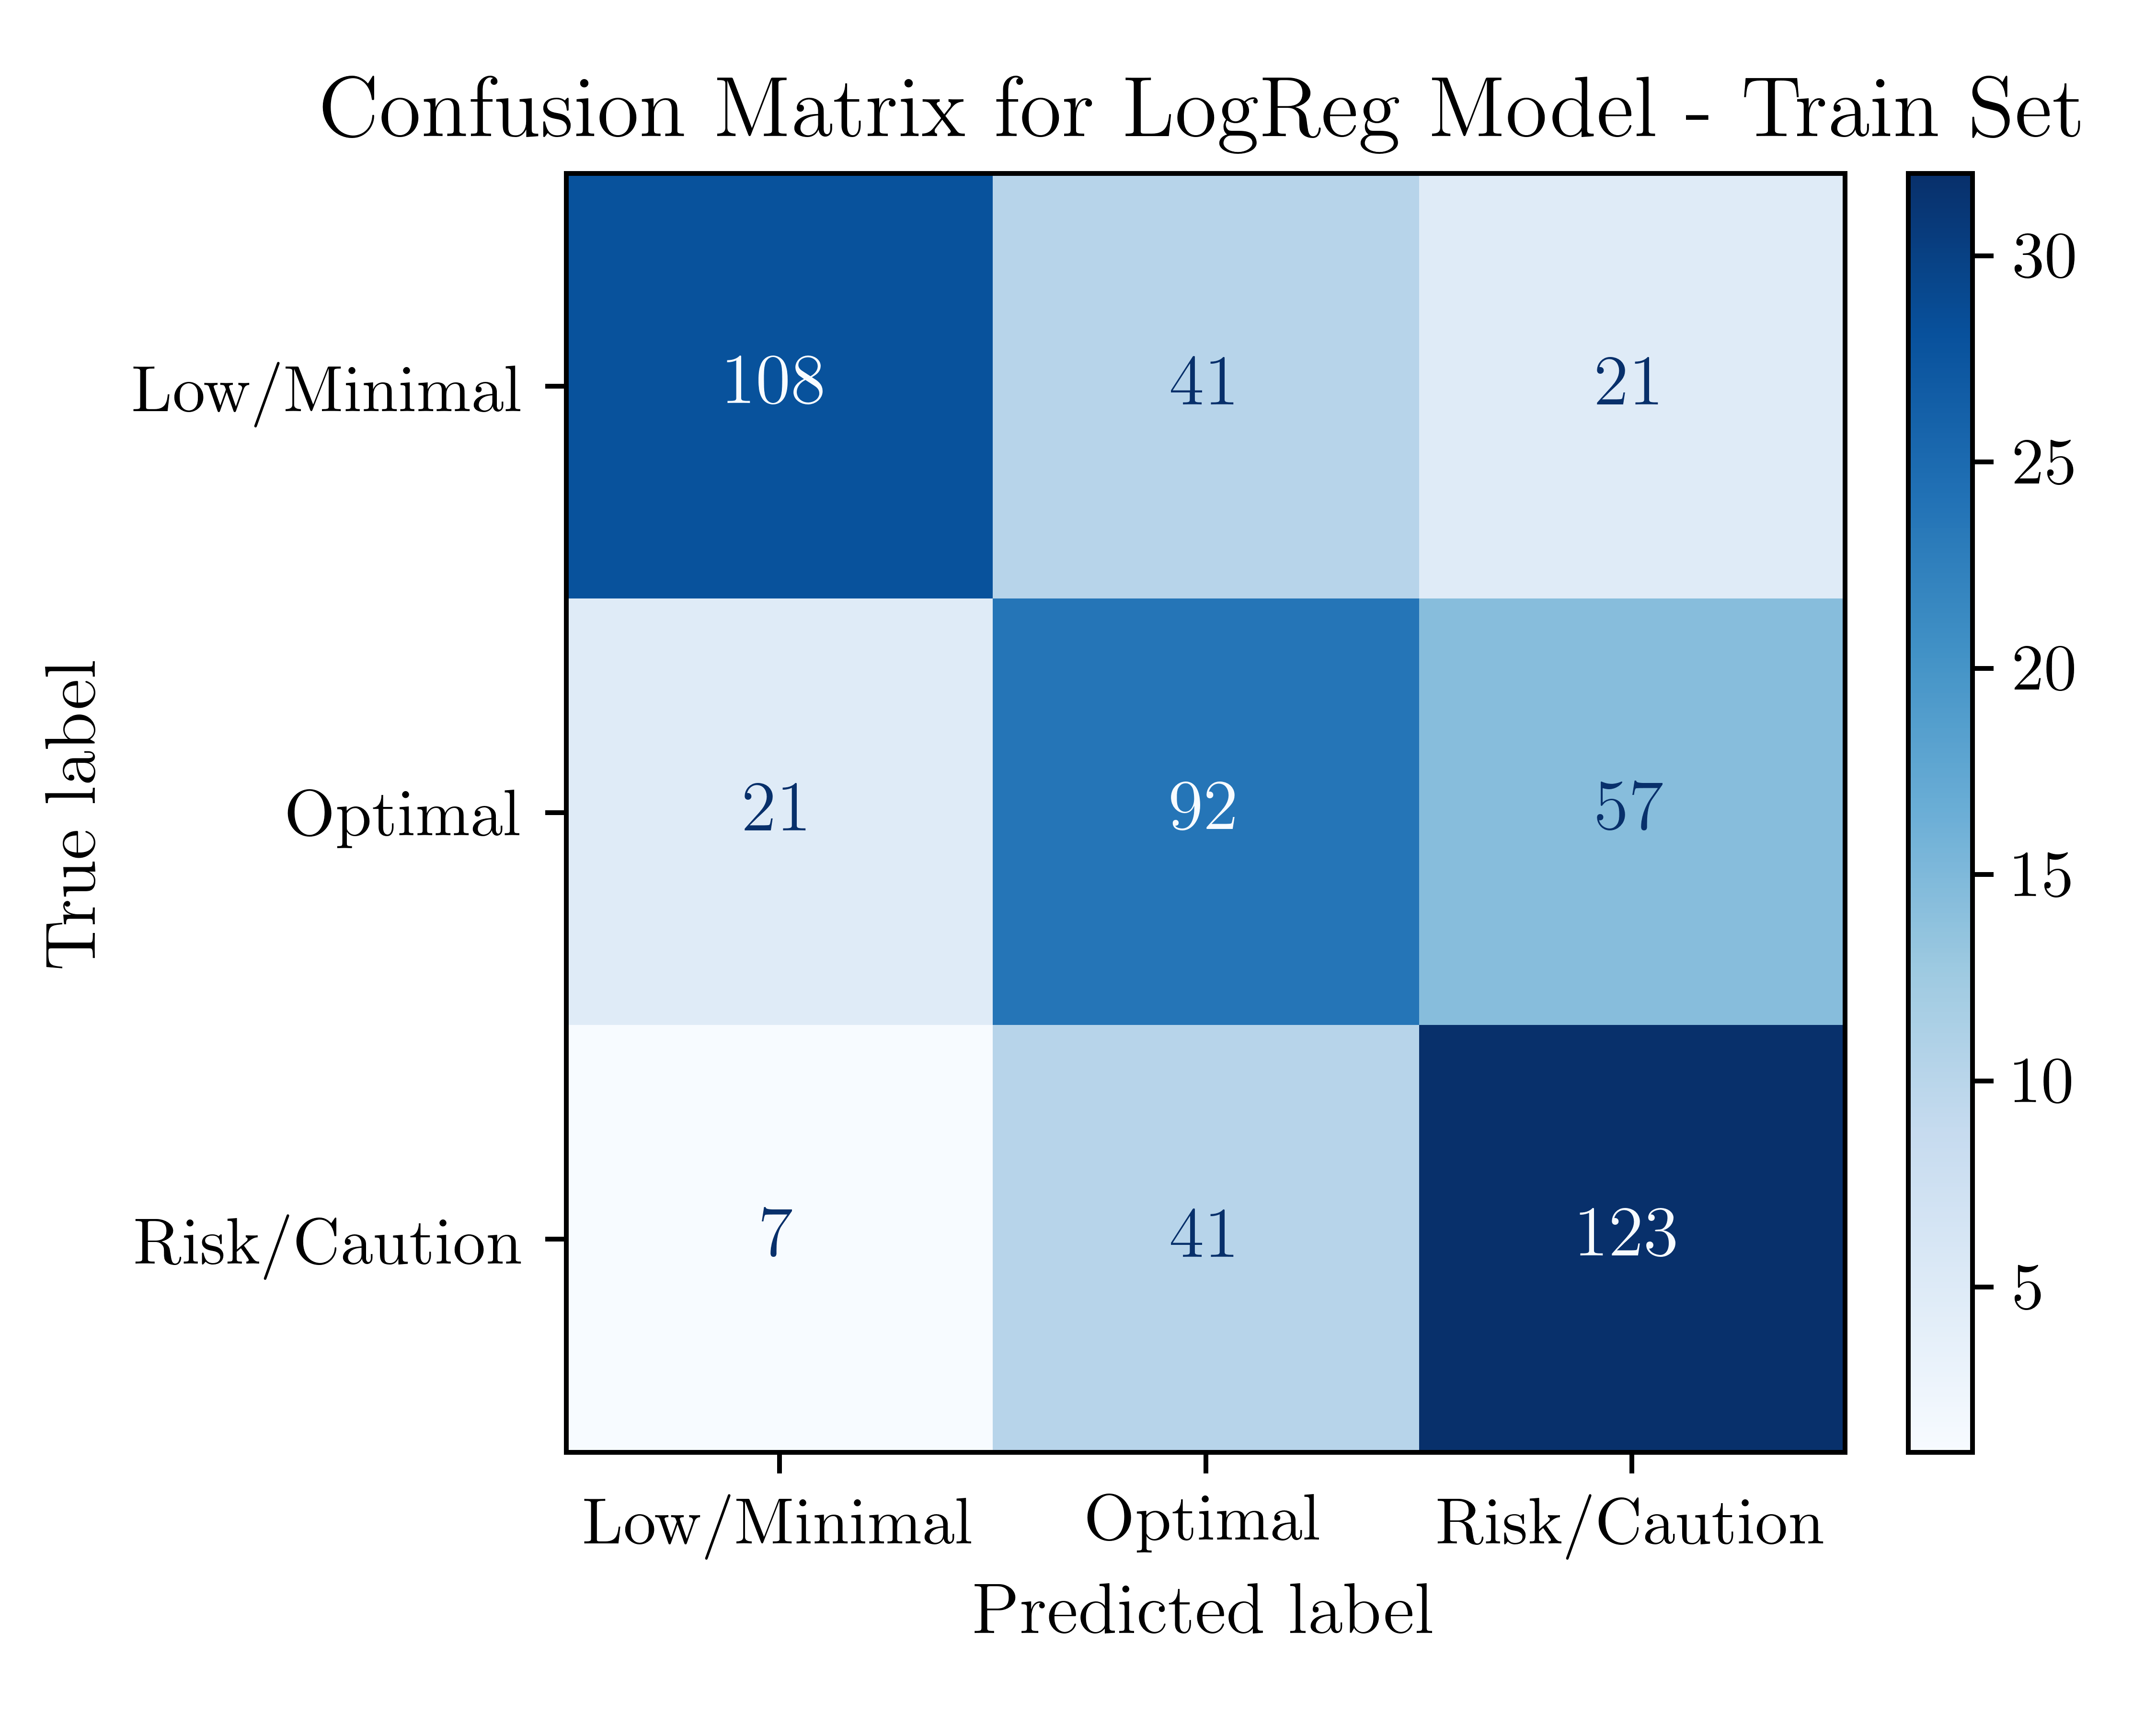
\includegraphics[width=1\linewidth]{assets/LOGR_confmatTrain.png}
    \caption{Confusion matrix for the training data of LogReg model.}
    \label{cf_train_LogReg}
\end{figure} %cm Train

\begin{table}[H]
\centering
\caption{Classification report for LogReg model performance evaluation on training data.}
\label{crTrainLogReg}
\begin{tabular}{lcccccc}
\toprule
\textbf{Class} & \textbf{Precision} & \textbf{Recall} & \textbf{F1-Score} & \textbf{Support} \\
\midrule
Low/Minimal & 0.79 & 0.64 & 0.71 & 170 \\
Optimal & 0.53 & 0.54 & 0.53 & 170 \\
Risk/Caution & 0.61 & 0.72 & 0.66 & 171 \\
\midrule
\textbf{Accuracy} &  &  & 0.63 & 511 \\
\textbf{Macro avg} & 0.64 & 0.63 & 0.63 & 511 \\
\textbf{Weighted avg} & 0.64 & 0.63 & 0.63 & 511 \\
\bottomrule
\end{tabular}
\end{table} %cr Train

\begin{figure}[H]
    \centering
    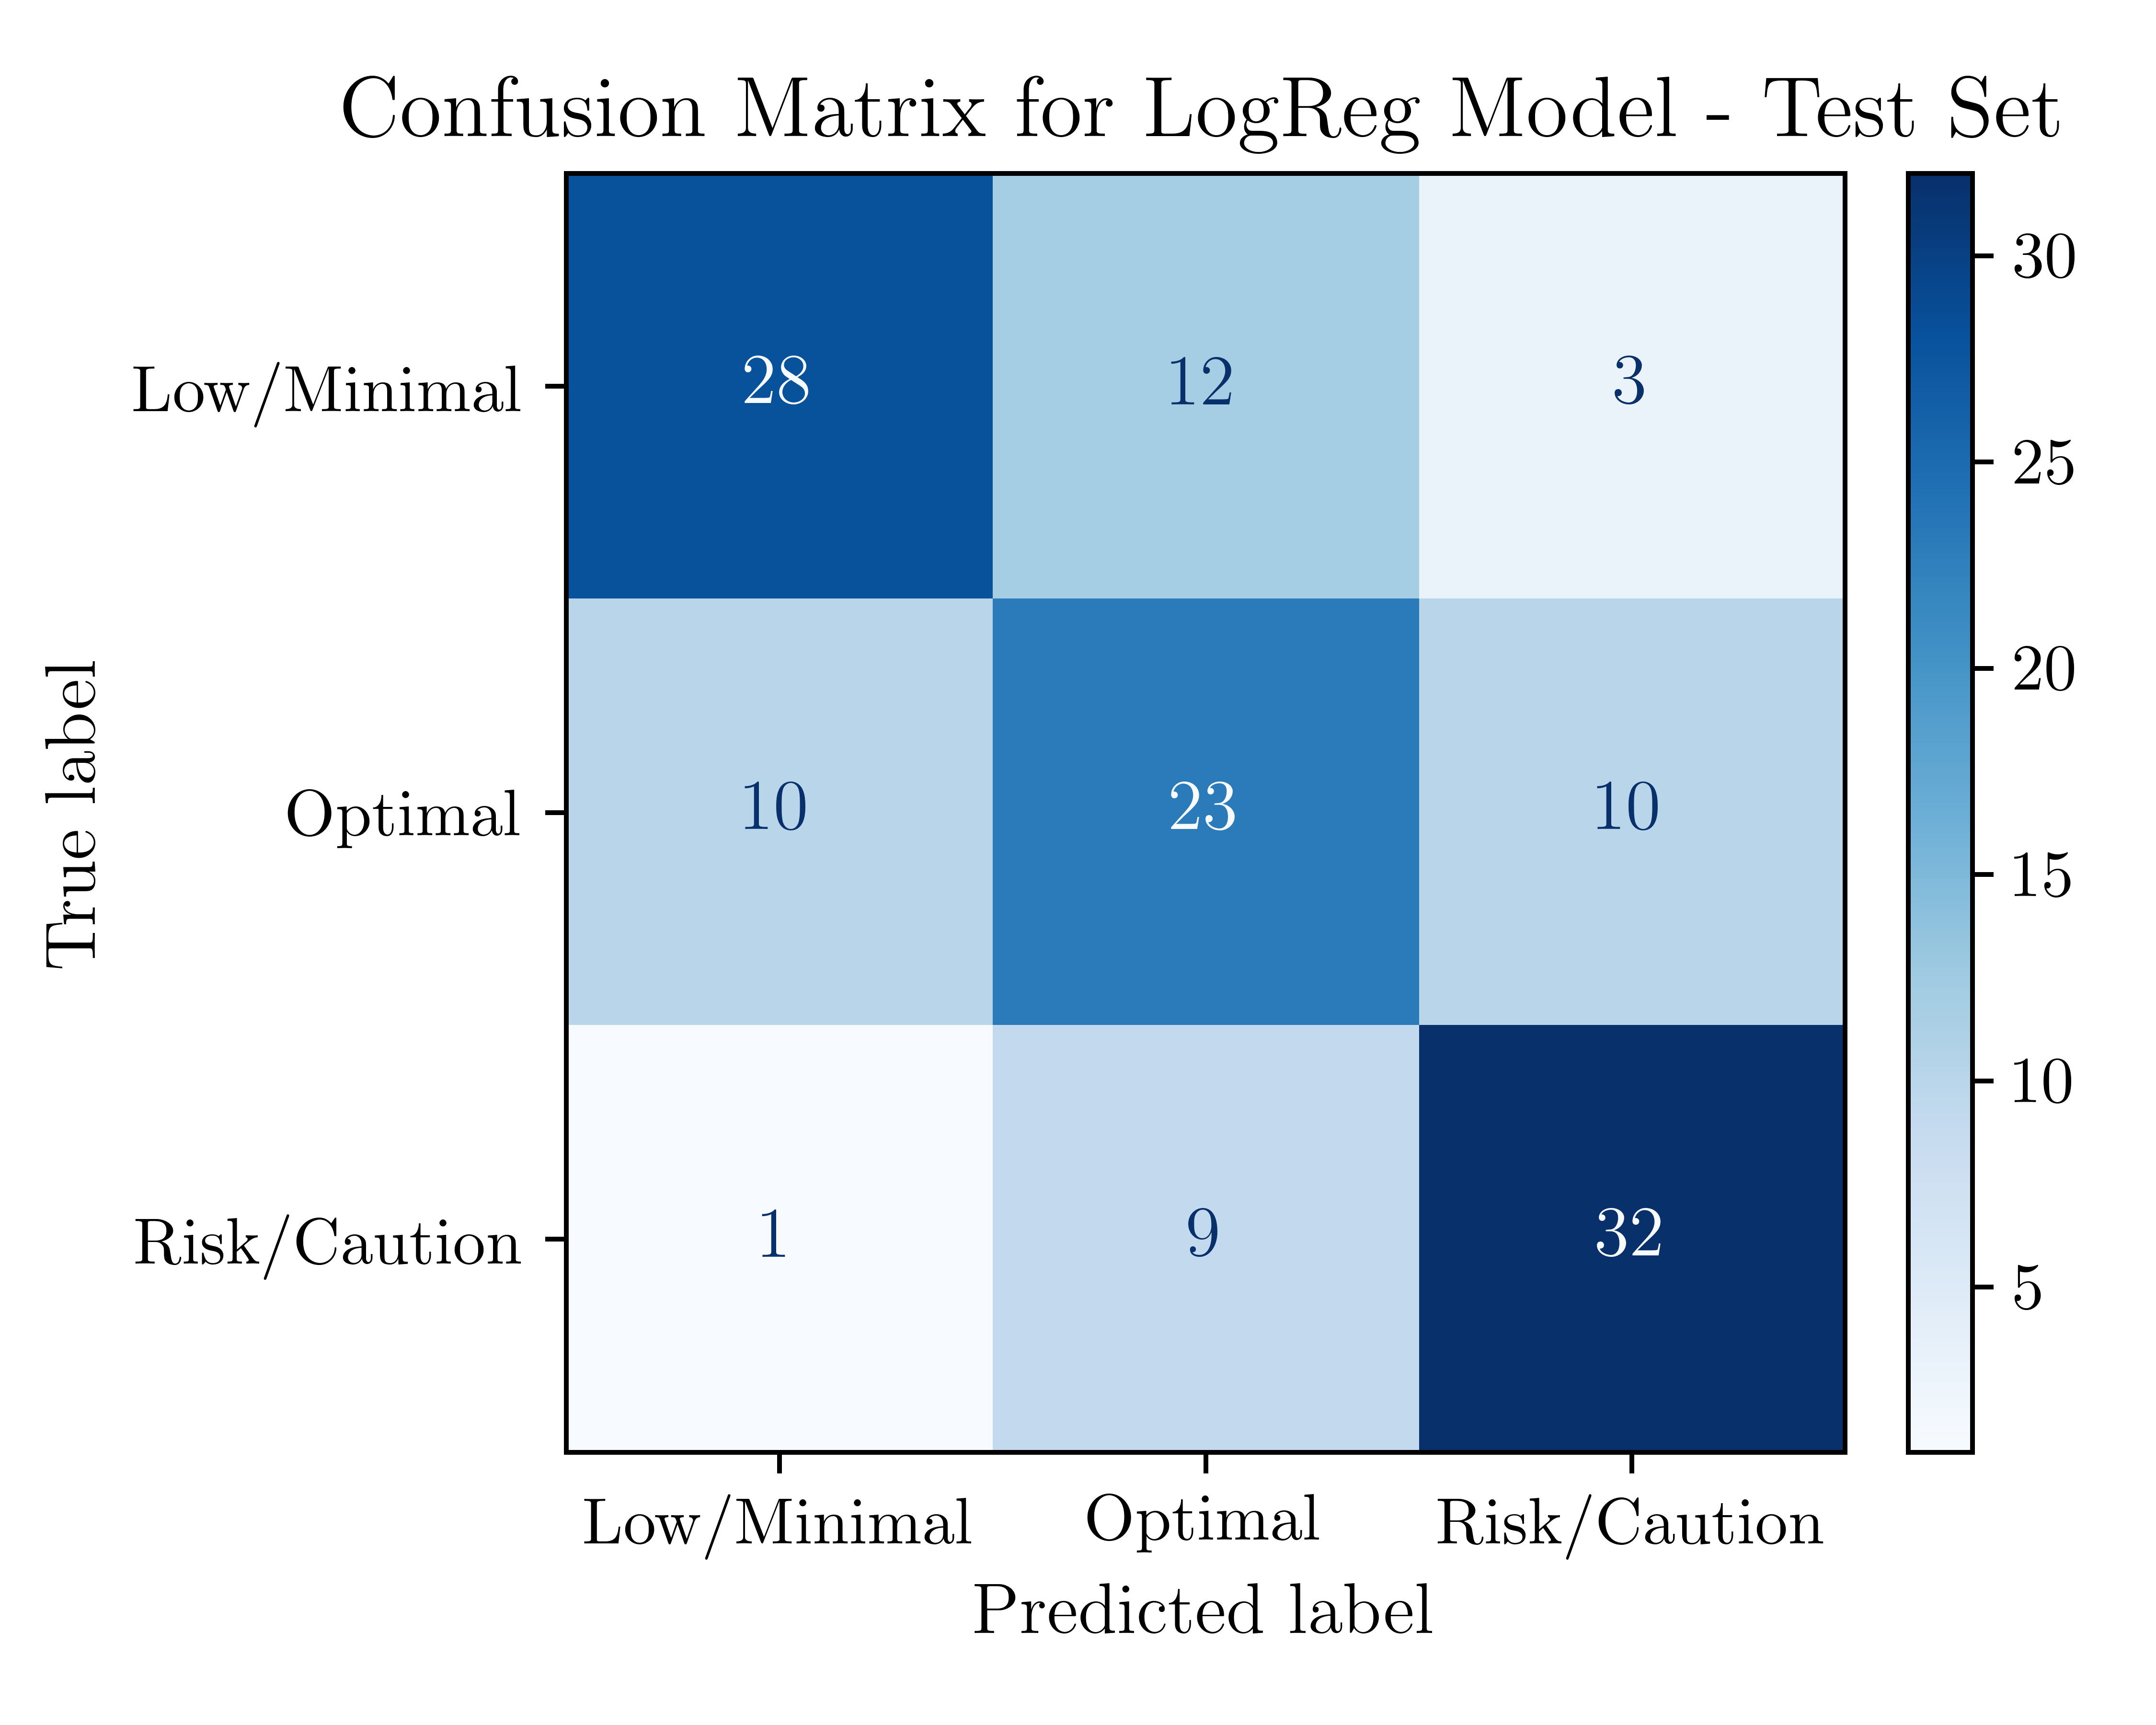
\includegraphics[width=1\linewidth]{assets/LOGR_confmatTest.png}
    \caption{Confusion matrix for the test data of LogReg model.}
    \label{cm_Test_LogReg}
\end{figure} %cm Test

\begin{table}[H]
\centering
\caption{Classification report for LogReg model performance evaluation on test data.}
\label{crTestLogREg}
\begin{tabular}{lcccccc}
\toprule
\textbf{Class} & \textbf{Precision} & \textbf{Recall} & \textbf{F1-Score} & \textbf{Support} \\
\midrule
Low/Minimal & 0.72 & 0.65 & 0.68 & 43 \\
Optimal & 0.52 & 0.52 & 0.53 & 43 \\
Risk/Caution & 0.71 & 0.76 & 0.74 & 42 \\
\midrule
\textbf{Accuracy} &  &  & 0.65 & 128 \\
\textbf{Macro avg} & 0.65 & 0.65 & 0.65 & 128 \\
\textbf{Weighted avg} & 0.65 & 0.65 & 0.65 & 128 \\
\bottomrule
\end{tabular}
\end{table} %cr Test

$\ $

\section{Support Vector Machine}

Given the increased complexity compared to LogReg, the support vector machine (SVM) model allows for manipulation of a larger number of hyperparameters, which consequently lead to longer computation times to achieve the best model. The hyperparameters used were Regularization Parameter (parameter that controls the penalty for misclassified training examples, i.e., cost function) ($C$), the Kernel Coefficient ($\gamma$), the kernel to be used, the highest degree possible (for a $poly$ kernel), and the value of the independent term (Coef$_0$), which controls the flexibility of the decision boundary for the $poly$ and $sigmoid$ kernels \cite{svm24}. The ranges of possible values can be assessed in Table \ref{parametrosSVM}.

\begin{table}[H]
\centering
\caption{SVM model hyperparameters search space.}
\label{parametrosSVM}
\begin{tabular}{ll}
\toprule
\textbf{Hyperparameter} & \textbf{Possible Values} \\
\midrule
$C$ & $[0, 100]$ \\ 
$\gamma$ & \{scale, auto, $0.1$, $0.01$, $0.001$\} \\ 
Kernel & \{linear, rbf, poly, sigmoid\} \\ 
Degree & \{1, 2, 3\} \\ 
Coef$_0$ & $[-5, 5]$ \\
\bottomrule
\end{tabular}
\end{table} %hyperparameters

As in the case for LogReg, an ideal class weight was estimated, however here only for 'Optimal' class, as it was the worst predicted class even at a training stage. The weight being smaller is penalizing the class, making it more likely to decide for one of the other classes when close to the decision boundary. The resulting regularization parameter is then defined by \cite{svm24},

$$C_{class} \leftarrow C \times w_{class}$$

The weight for the 'Optimal' class that retrieved the highest accuracy was estimated as shown in Fig.~\ref{svm_weight} ($w_{Optimal}=0.8$). 

\begin{figure}[H]
    \centering
    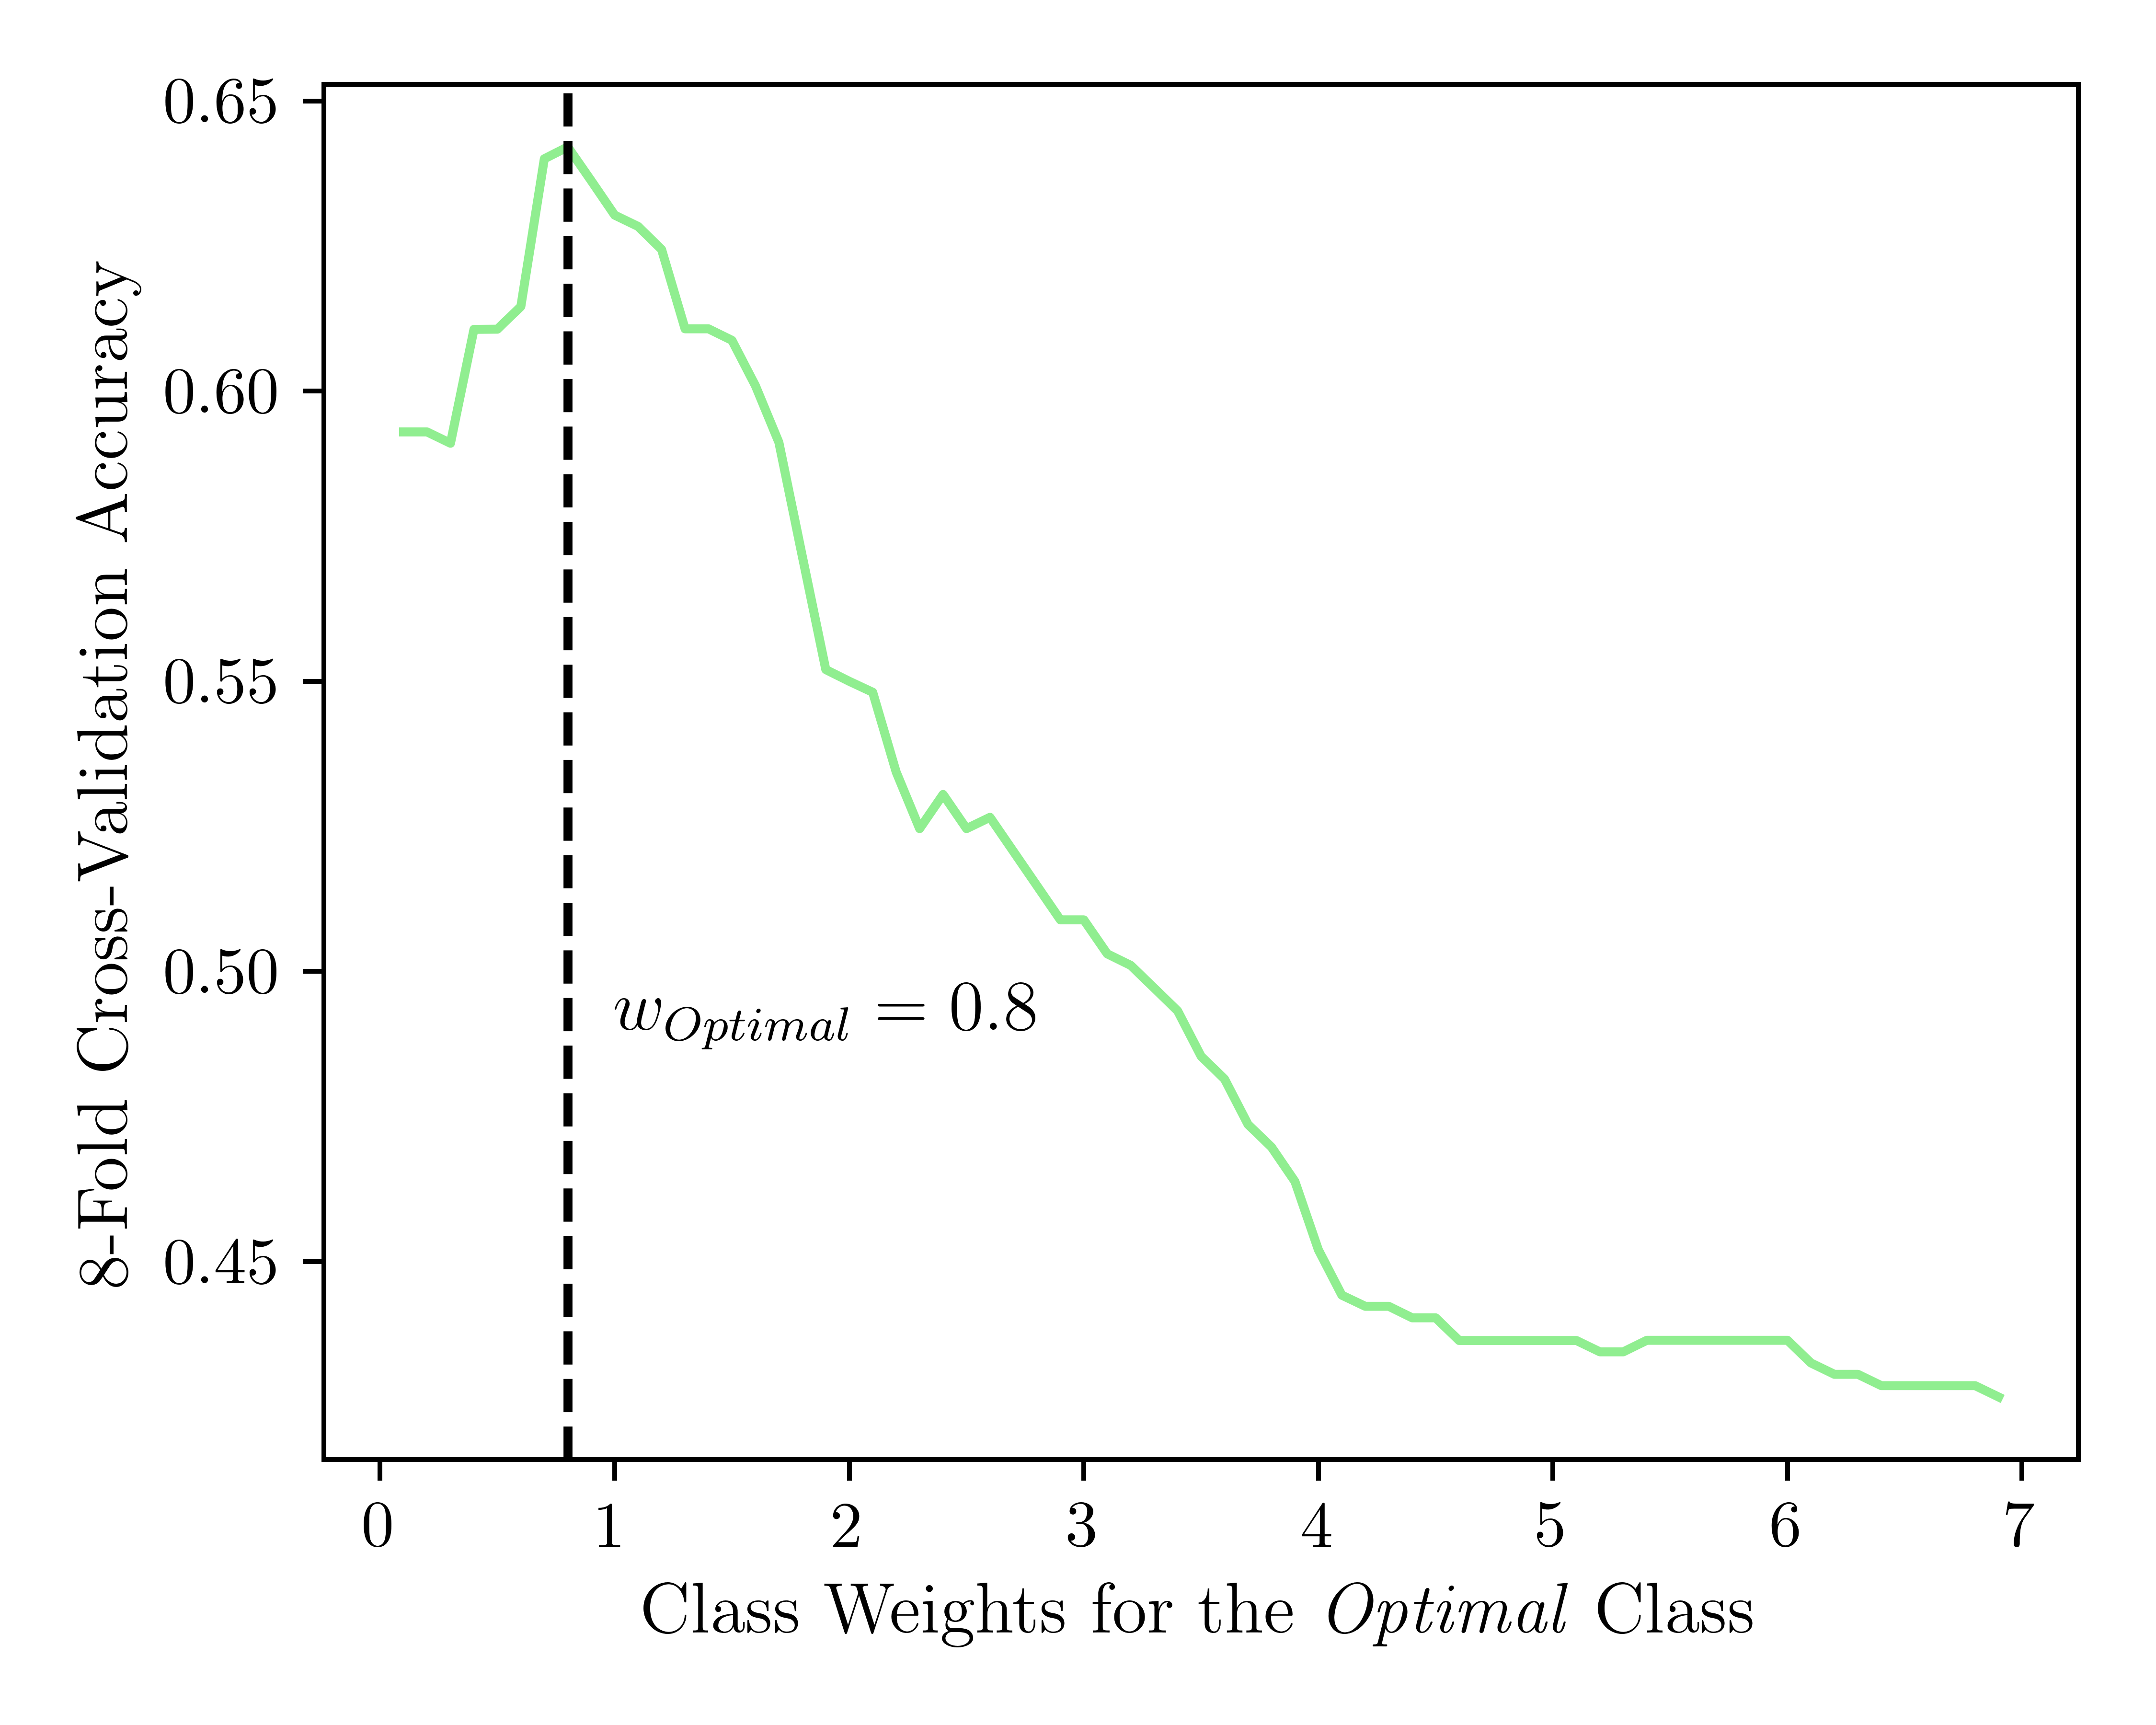
\includegraphics[width=1\linewidth]{assets/SVM_OptimalWeight.png}
    \caption{Effect of the 'Optimal' class weight on SVM model accuracy.}
    \label{svm_weight}
\end{figure} %class weight

The remaining classes kept the initially attributed unitary weight. The best parameters found, for this weights, were $C$ 6.93, $\gamma$ auto ($1/n_{features}$), and kernel RBF (Radial Basis Function).

$$\text{RBF kernel: } \exp(-\gamma ||x - x'||^2)$$ %RBF

In this case, the learning curves  for both the training and cross-validation sets (Fig. \ref{svm_learningcurve}) converge, with no signs of overfitting. However, it could be beneficial to expand the training dataset further, as the cross-validation score continues to improve. This suggests that the model might still benefit from more data, which could enhance its ability to generalize better.

\begin{figure}[H]
    \centering
    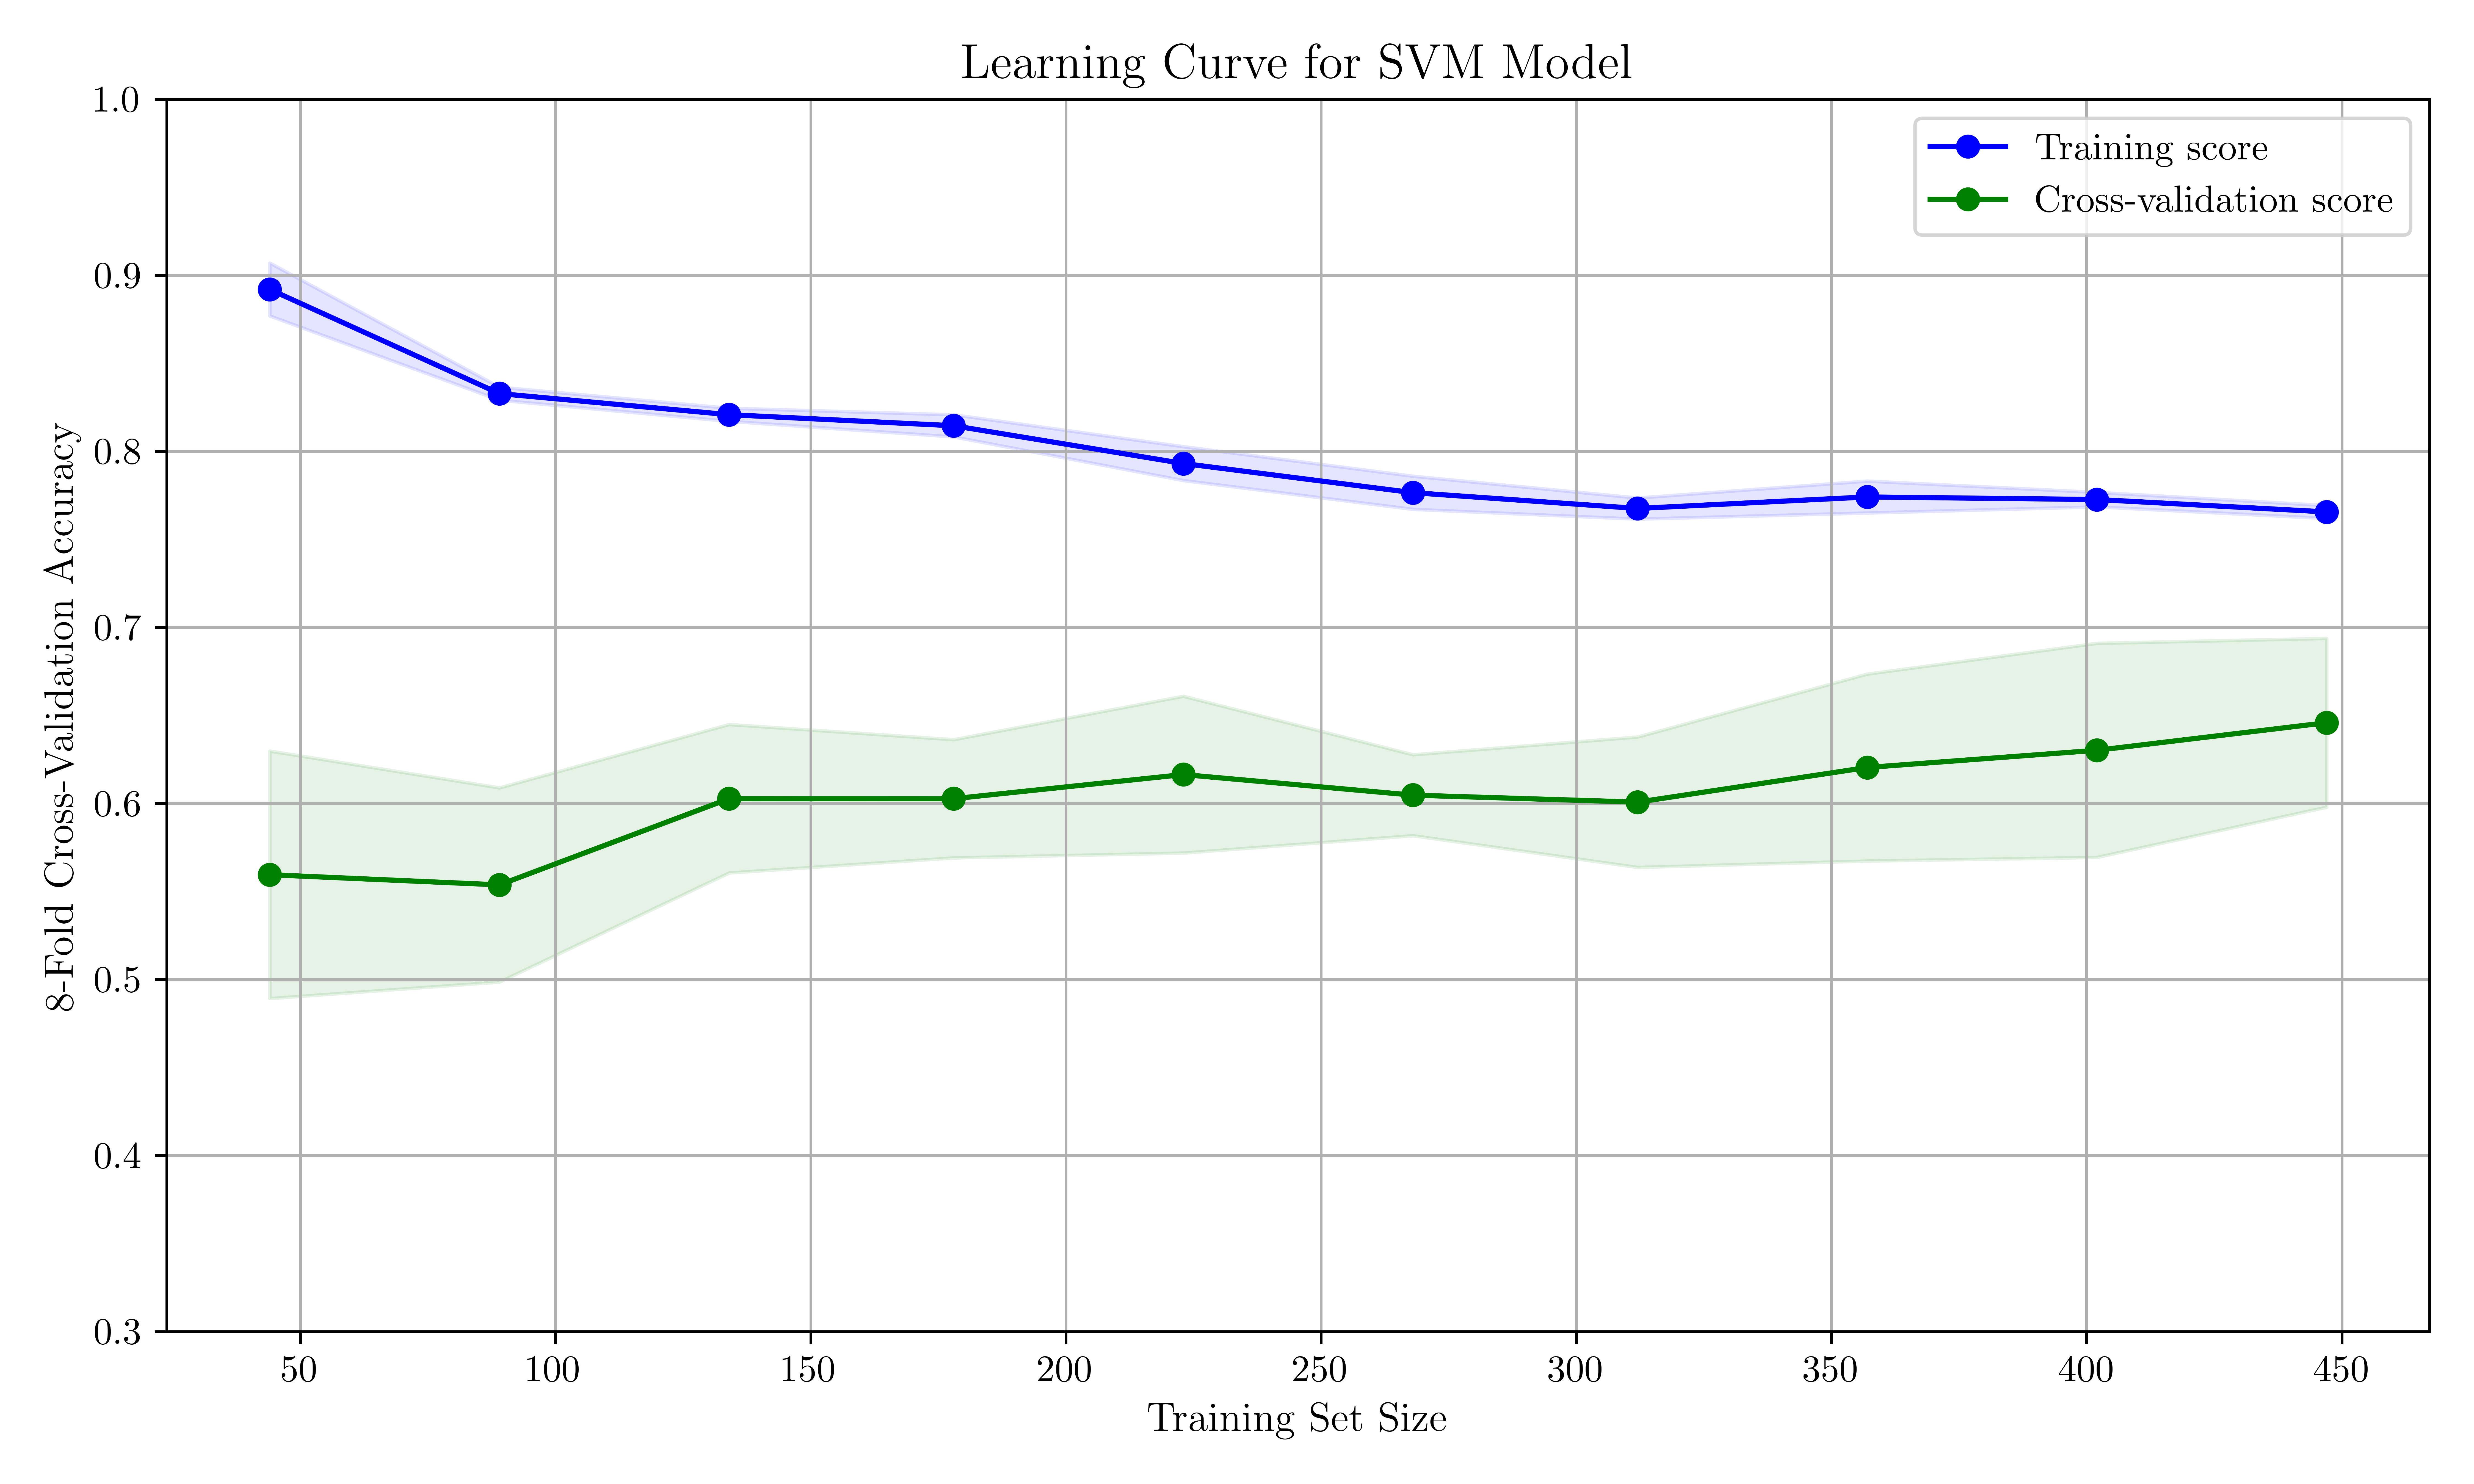
\includegraphics[width=1\linewidth]{assets/SVM_LearningCurve.png}
    \caption{SVM model performance using learning curve representation across varying training data sizes.}
    \label{svm_learningcurve}
\end{figure} % learning curve

The confusion matrices for both training (Fig.~\ref{svm_cm_train}) and testing datasets (Fig.~\ref{svm_cm_test}) show a good performance in the classification of all classes, especially for those in the extremities (as already verified in the previous model).

The classification reports of the training (Table~\ref{crTrainSVM}) and testing datasets (Table~\ref{crTestSVM}) show consistent results among them. However, it is noteworthy the low value of Recall for the 'Optimal' class in both cases, indicating several misclassification occurrences (observations that should be 'Optimal' but were classified as one of the other classes). 

\begin{figure}[H]
    \centering
    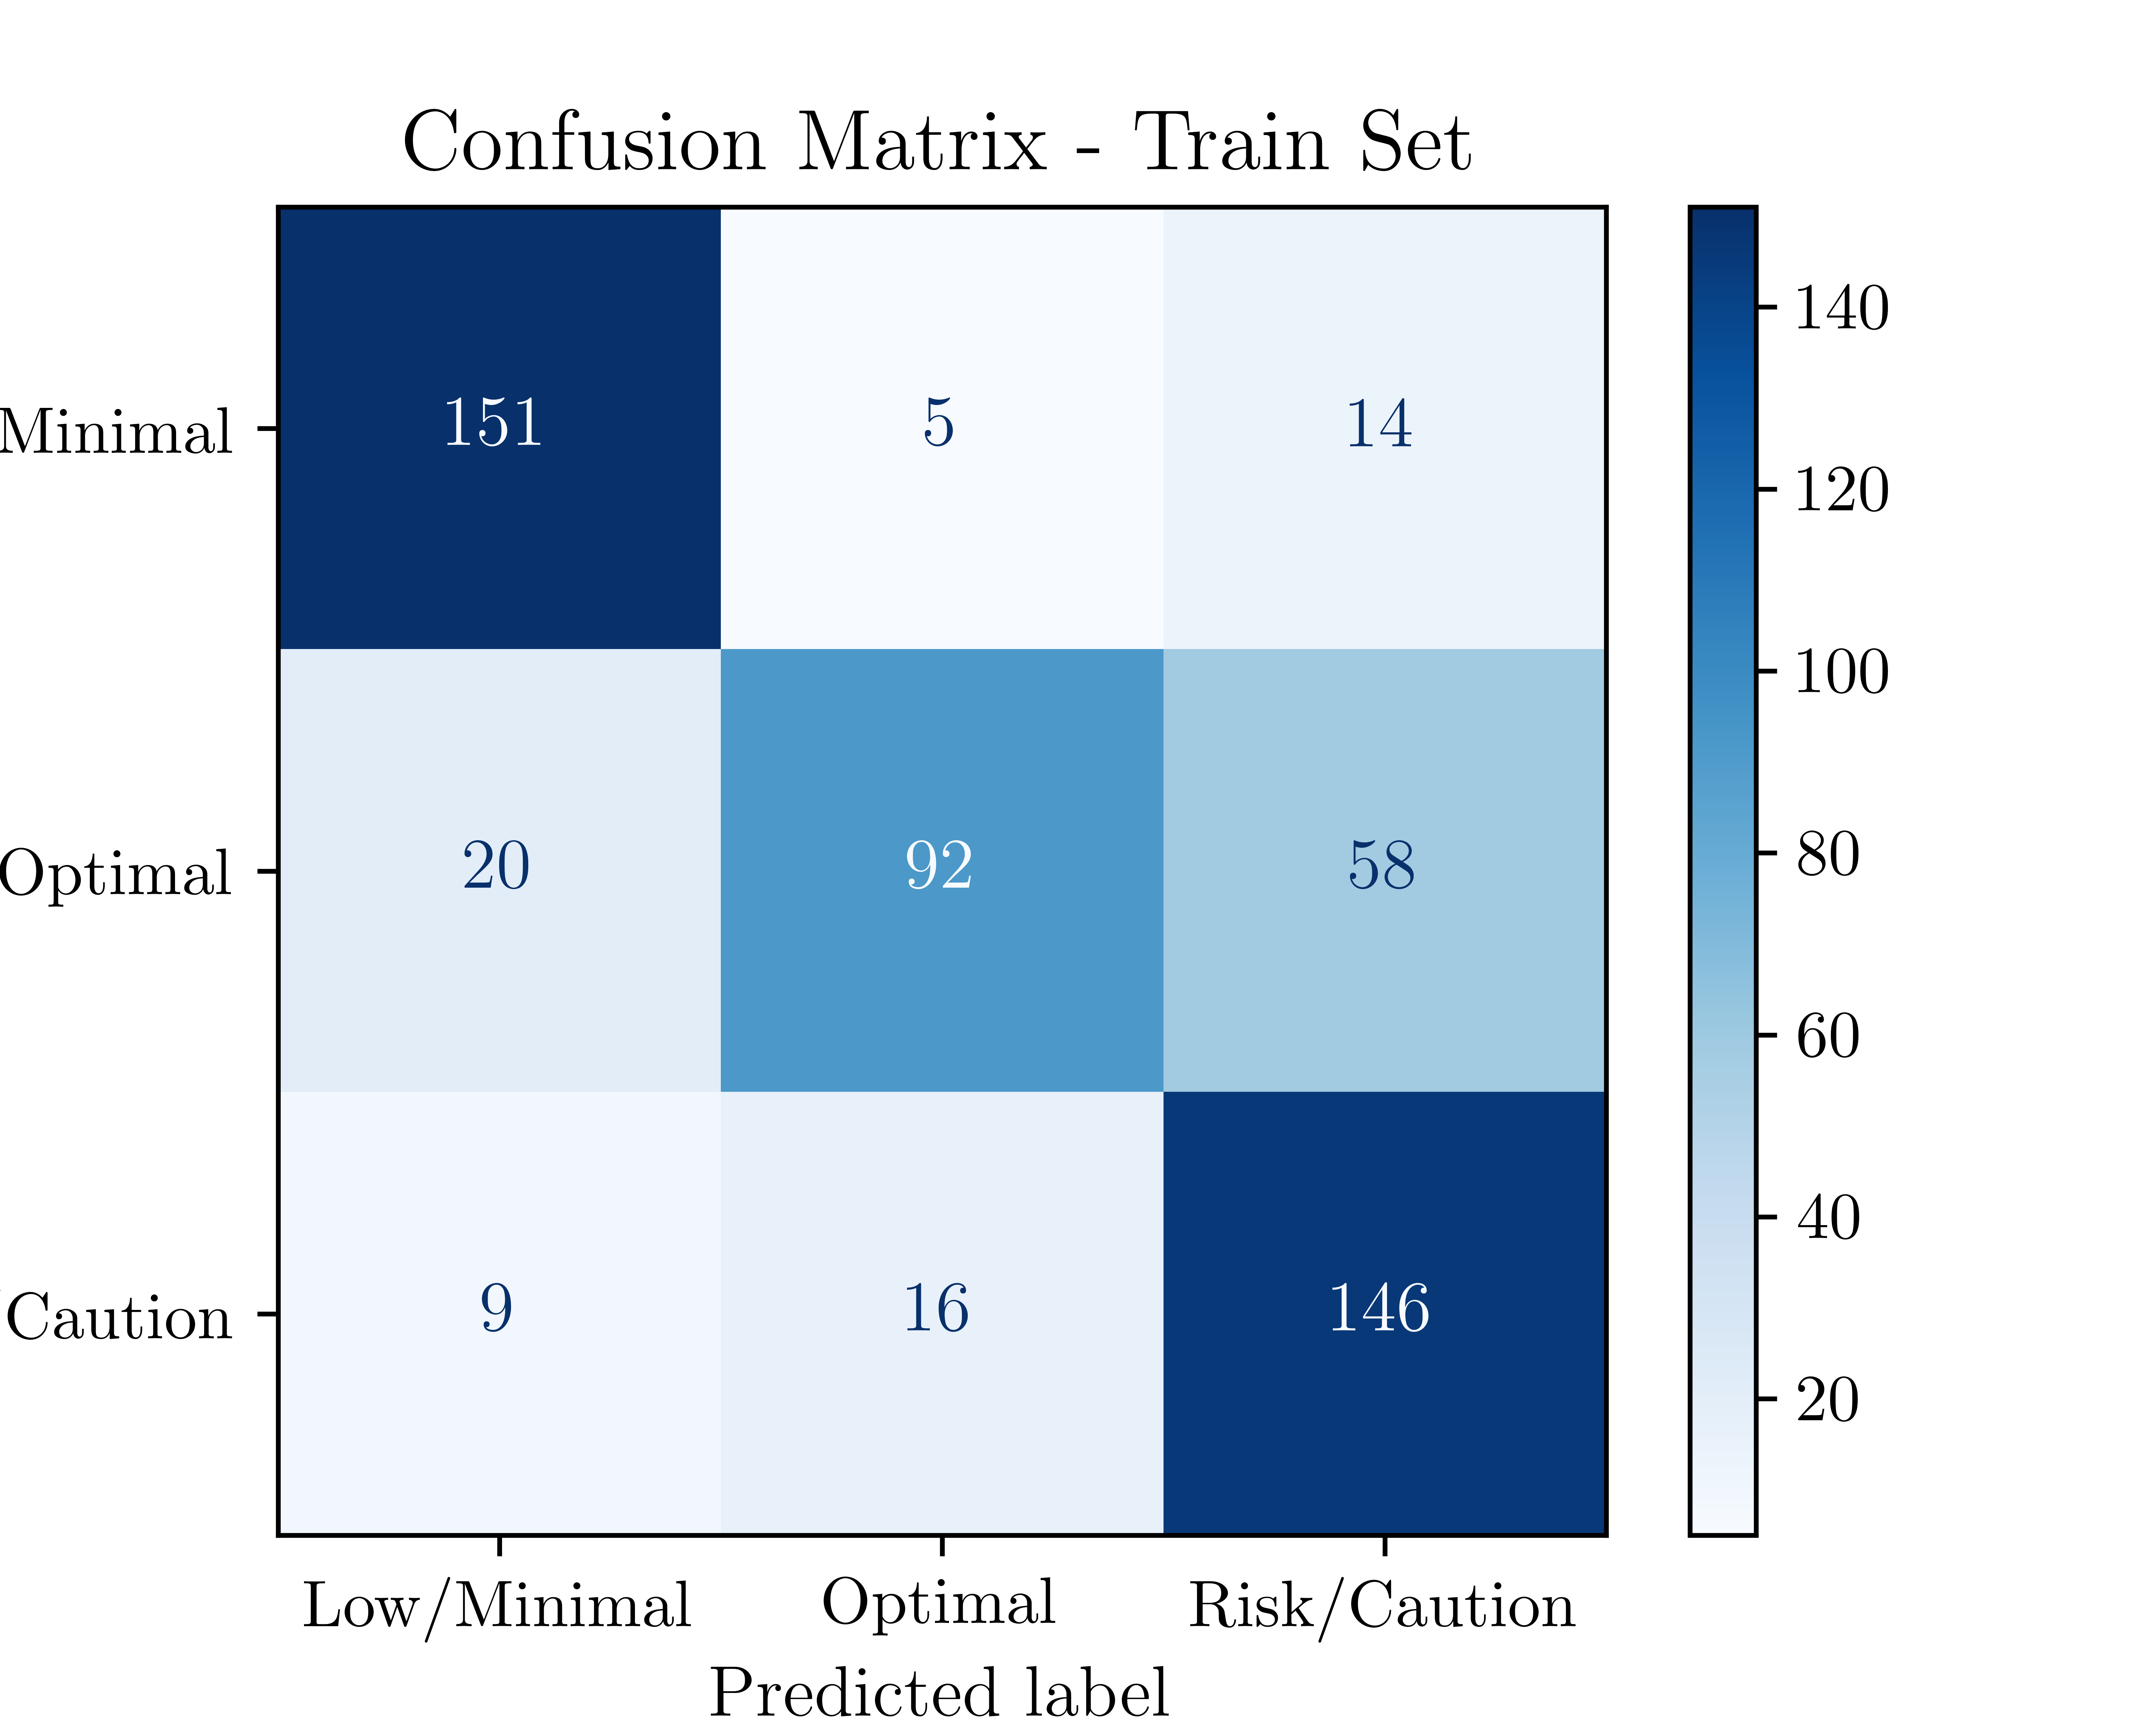
\includegraphics[width=1\linewidth]{assets/SVM_ConfusionMatrixTrain.png}
    \caption{Confusion matrix for the training data of SVM model}
    \label{svm_cm_train}
\end{figure} %cm Train

\begin{table}[H]
\centering
\caption{Classification report for SVM model performance evaluation on training data.}
\label{crTrainSVM}
\begin{tabular}{lcccccc}
\toprule
\textbf{Class} & \textbf{Precision} & \textbf{Recall} & \textbf{F1-Score} & \textbf{Support} \\
\midrule
Low/Minimal & 0.84 & 0.89 & 0.86 & 170 \\
Optimal & 0.81 & 0.54 & 0.65 & 170 \\
Risk/Caution & 0.67 & 0.85 & 0.75 & 171 \\
\midrule
\textbf{Accuracy} &  &  & 0.76 & 511 \\
\textbf{Macro avg} & 0.77 & 0.76 & 0.75 & 511 \\
\textbf{Weighted avg} & 0.77 & 0.76 & 0.75 & 511 \\
\bottomrule
\end{tabular}
\end{table} %cr Train

\begin{figure}[H]
    \centering
    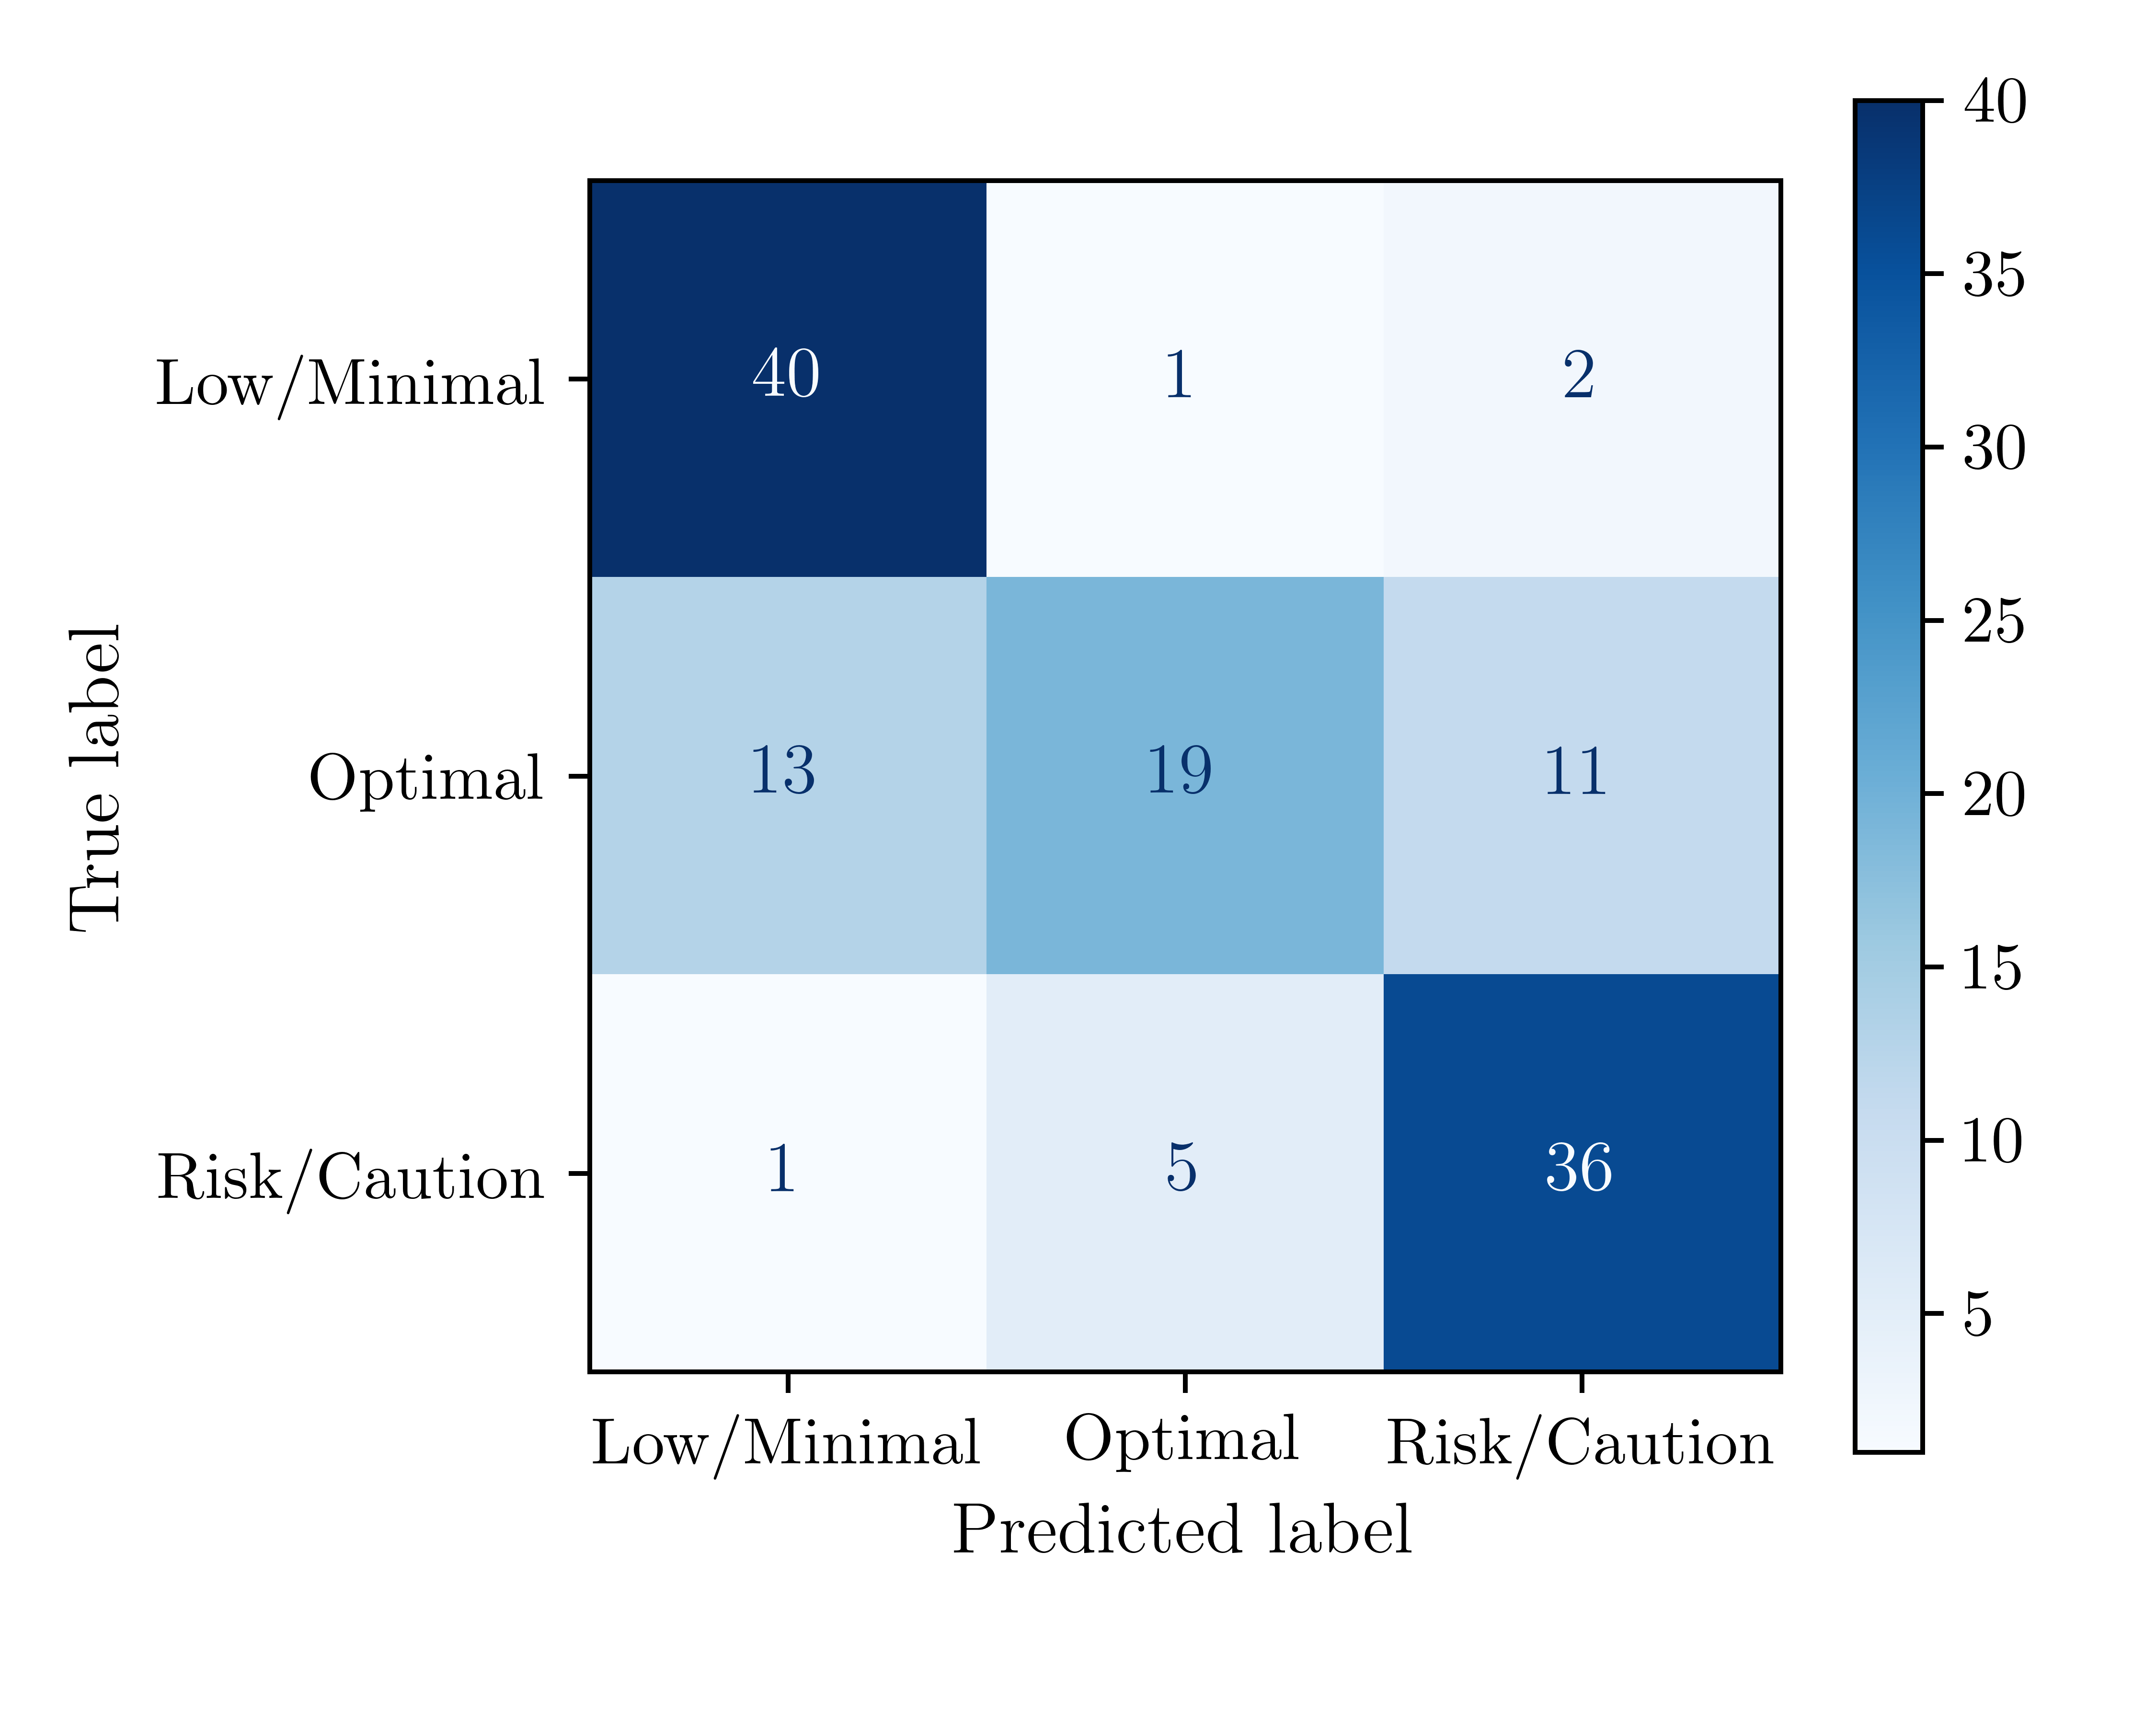
\includegraphics[width=1\linewidth]{assets/SVM_ConfusionMatrixTest.png}
    \caption{Confusion matrix for the test data of SVM model}
    \label{svm_cm_test}
\end{figure} %cm Test

\begin{table}[H]
\centering
\caption{Classification report for SVM model performance evaluation on test data.}
\label{crTestSVM}
\begin{tabular}{lcccccc}
\toprule
\textbf{Class} & \textbf{Precision} & \textbf{Recall} & \textbf{F1-Score} & \textbf{Support} \\
\midrule
Low/Minimal & 0.74 & 0.93 & 0.82 & 43 \\
Optimal & 0.76 & 0.44 & 0.56 & 43 \\
Risk/Caution & 0.73 & 0.86 & 0.79 & 42 \\
\midrule
\textbf{Accuracy} &  &  & 0.74 & 128 \\
\textbf{Macro avg} & 0.75 & 0.74 & 0.72 & 128 \\
\textbf{Weighted avg} & 0.75 & 0.74 & 0.72 & 128 \\
\bottomrule
\end{tabular}
\end{table} %cr Test

\section{Decision Tree} \label{dtree_section}

The decision tree model was developed considering the hyperparameters available and setting ranges for the possible values to be estimated \cite{dtree17}. The ranges were selected taking in consideration the need to minimize the risk of overfitting. The maximum depth illustrates how deep the tree goes, and can be a sign of overfitting if it 'grows' too long. The minimum sample split constrains the tree in the number of splits allowed, as it requires more samples at each child node. A similar hyperparameter is minimum sample per leaf, meaning the minimum number of samples at any end node (making them more relevant). The split criterion evaluates the quality of a split when building the decision tree. The hyperparameters and ranges selected are presented in Table~\ref{parametrosDTree}.

\begin{table}[H]
\centering
\caption{Decision tree model hyperparameters search space.}
\label{parametrosDTree}
\begin{tabular}{ll}
\toprule
\textbf{Hyperparameter} & \textbf{Possible Values} \\
\midrule
Split Criterion & \{gini, entropy\} \\ 
Max Depth & $[2, 3, \dots, 8]$ \\ 
Min Samples to Split & $[5, 6, \dots, 20]$ \\ 
Min Samples per Leaf & $[3, 4, \dots, 10]$ \\
\bottomrule
\end{tabular}
\end{table} %hyperparameters

The maximum tree depth selected was 4, minimum samples to split 11, minimum samples per leaf 7, and the split criterion entropy ($H$), given by

$$H(\text{node}) = - \sum_{\text{Class }_j} p(\text{Class}_j | \text{node}) \log p(\text{Class}_j | \text{node})$$

The optimized DTree resulted in the structure as seen in Fig.~\ref{dtree_tree}.

\begin{figure}[H]
    \centering
    \includegraphics[width=1\linewidth]{assets/DTREE_Tree.png}
    \caption{Visualization of the decision tree model after optimization using randomized search.}
    \label{dtree_tree}
\end{figure} %dtree fig

The decision paths are characterized by the certainty in each node, highlighted by the color saturation for each of the classes ('Low/Minimal', 'Optimal', 'Risk/Caution'). The diminished proportion of end nodes with higher color saturation for 'Optimal' when comparing with the other classes is noteworthy, and consistent with the observations for the remaining models.

The learning curves were assessed from Fig.~\ref{dtree_lcurve}, which shows a significant improvement up until a training set size of 250, but with there's no significant gain with increasing set sizes, with the learning curves even slightly diverging at 450 samples.

\begin{figure}[H]
    \centering
    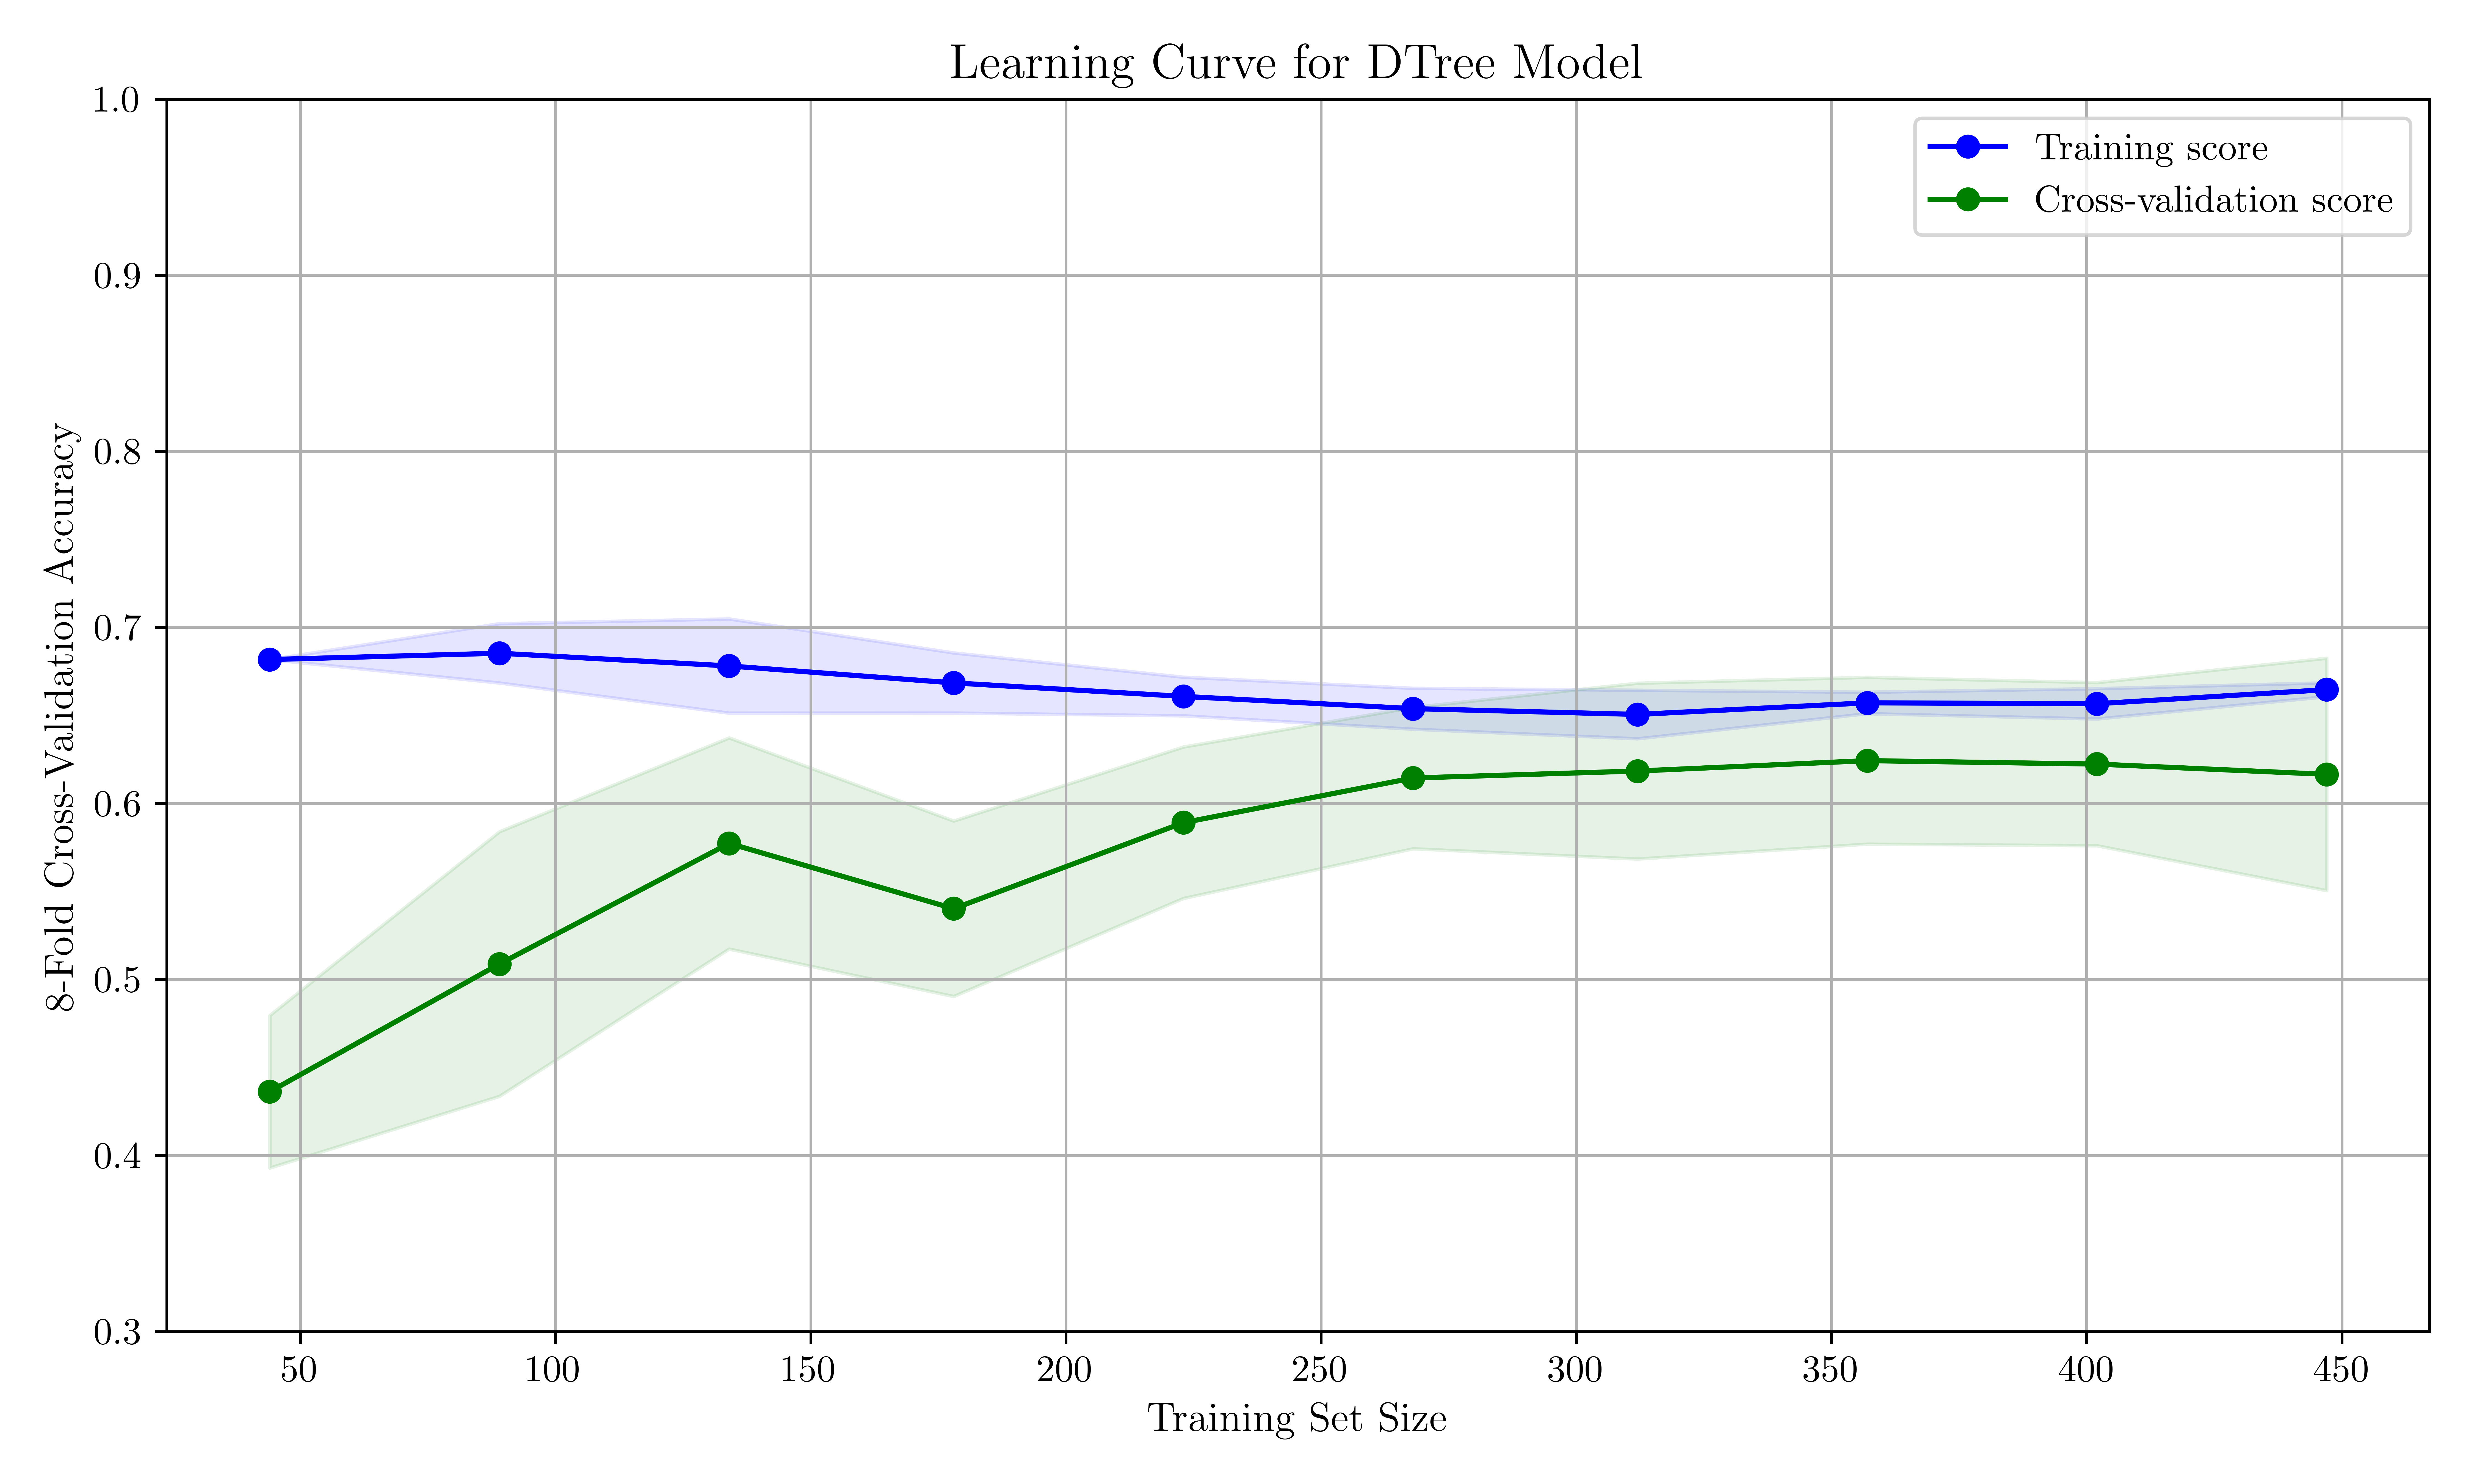
\includegraphics[width=1\linewidth]{assets/DTREE_LearningCurve.png}
    \caption{Analysis of decision tree model performance using learning curve representation across varying training data sizes.}
    \label{dtree_lcurve}
\end{figure} %learning curve

From the confusion matrices for training (Fig.~\ref{dtree_cmtrain}) and testing datasets (Fig.~\ref{dtree_cmtest}) it is visible that the model had some difficulty between the 'Optimal' and 'Risk/Caution' classes, but with a satisfying prediction performance for 'Low/Minimal'.

\begin{figure}[H]
    \centering
    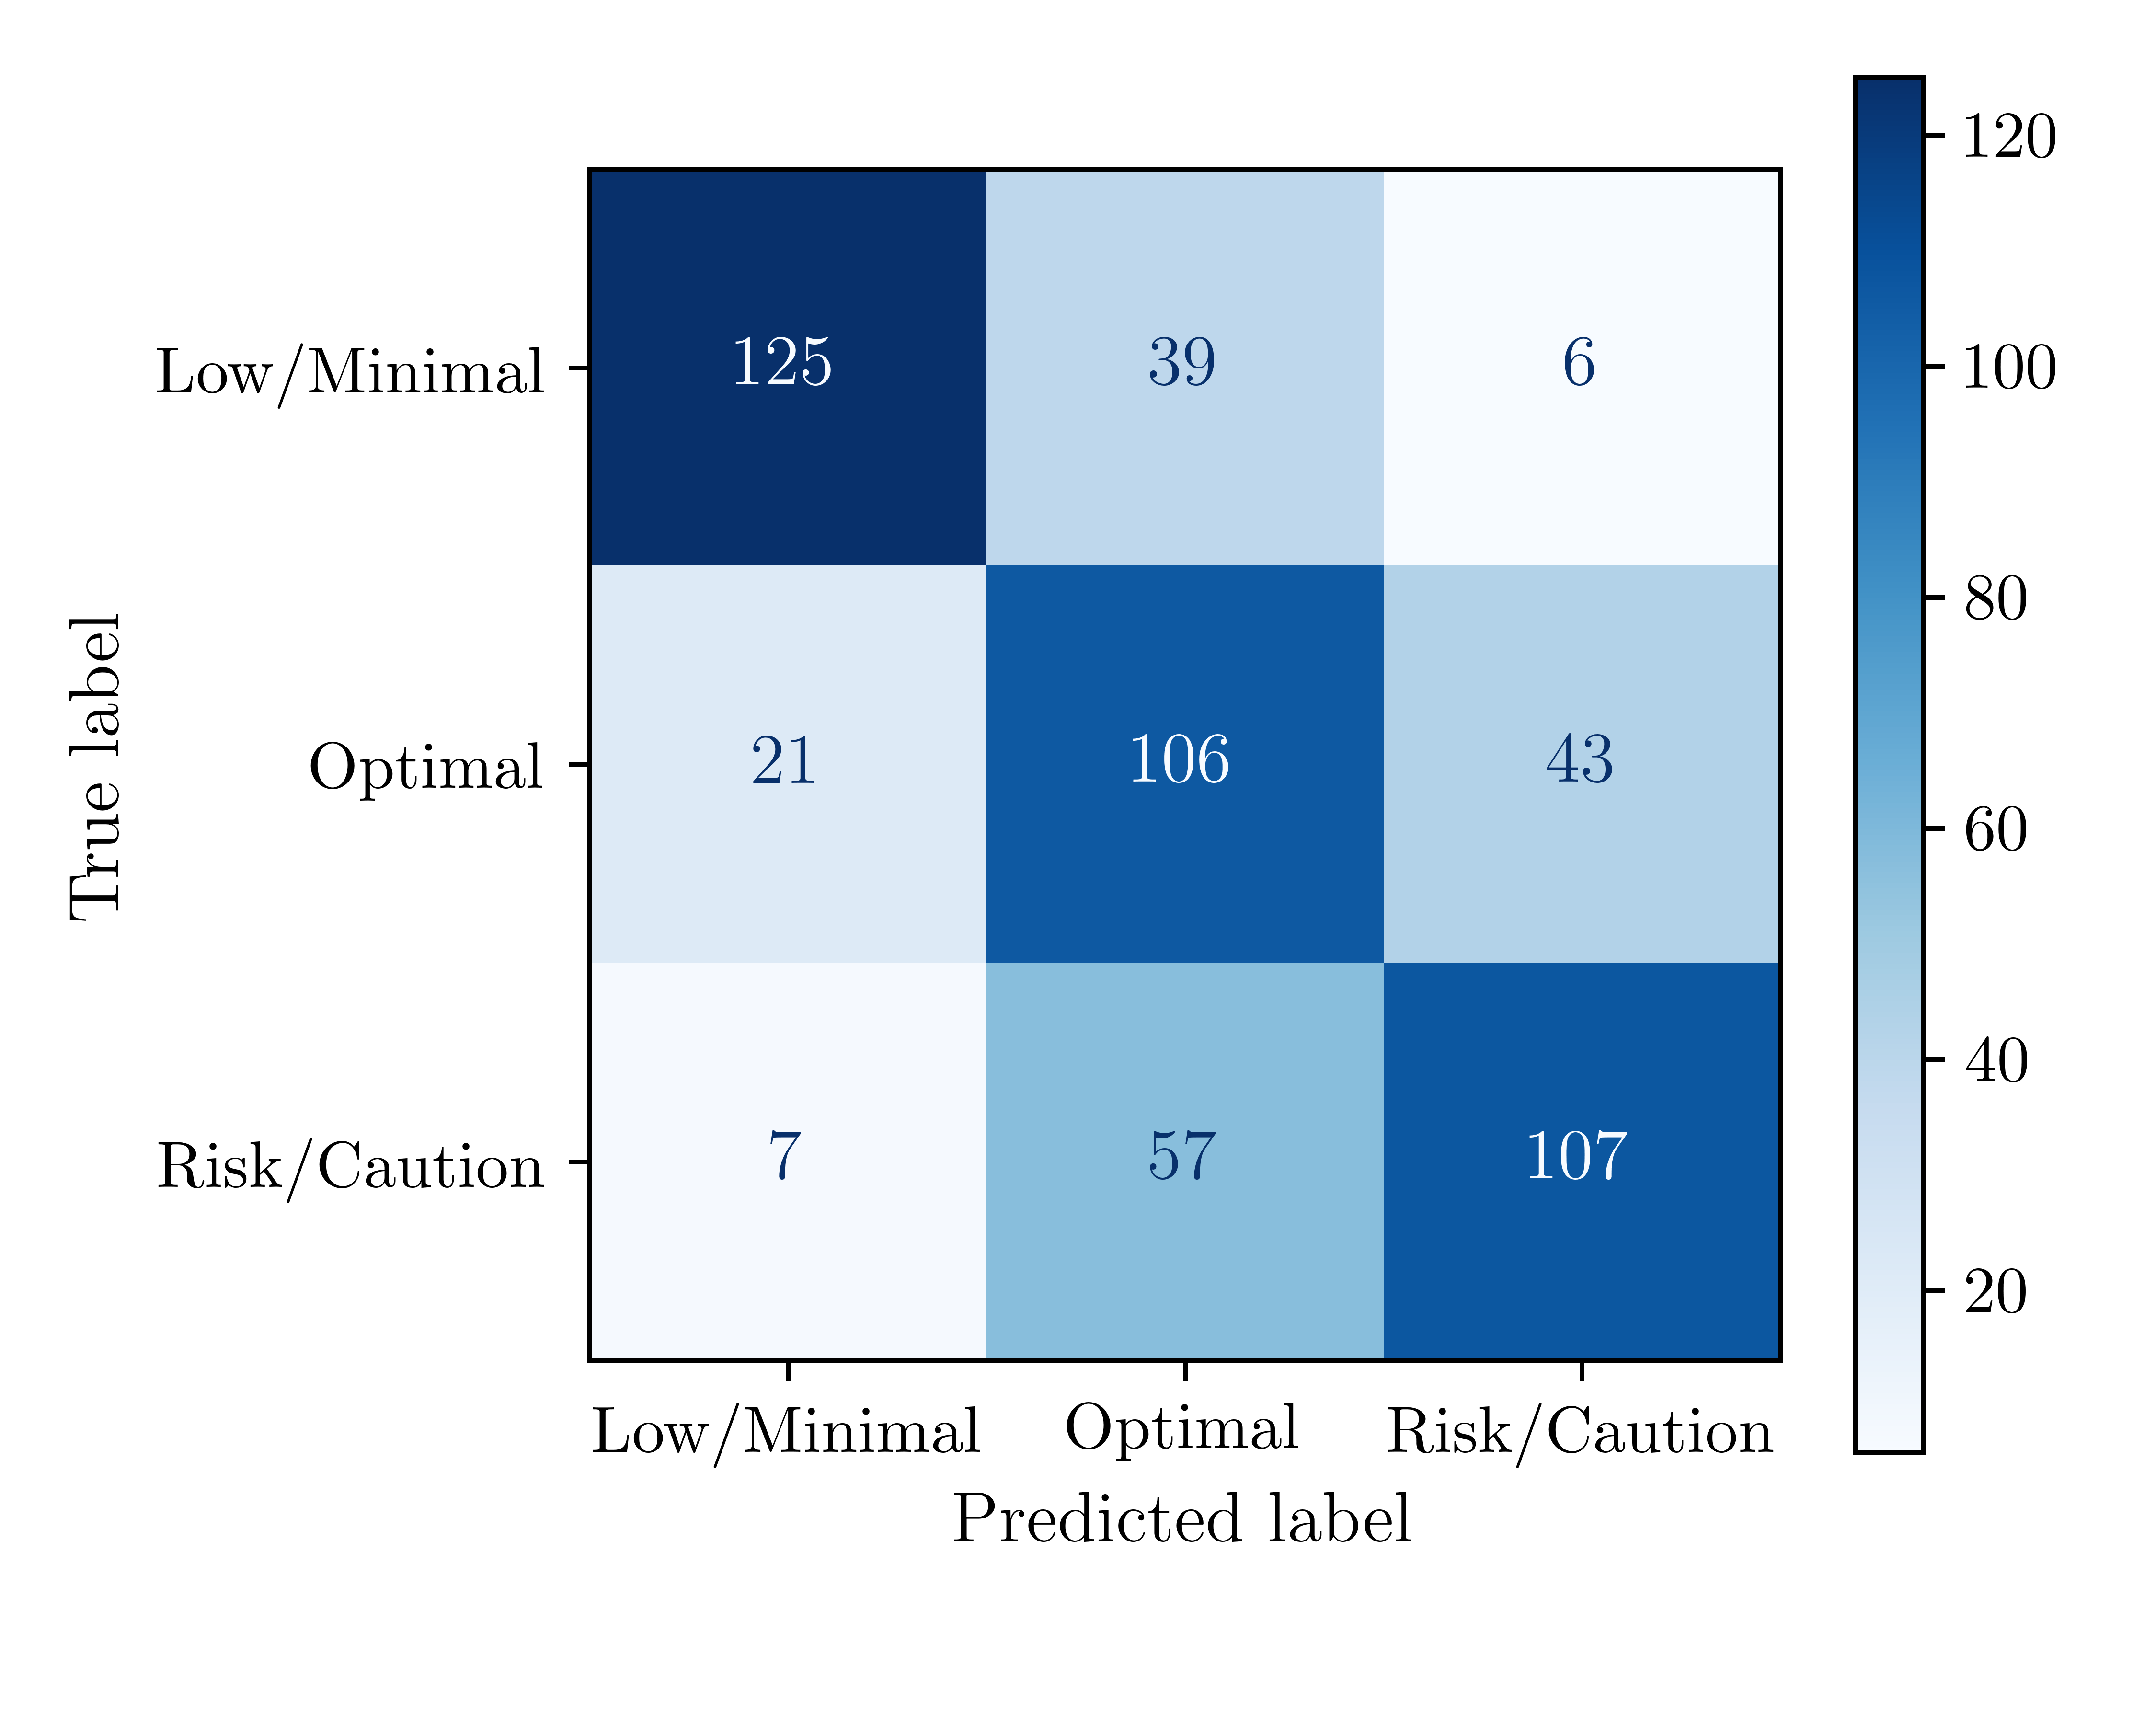
\includegraphics[width=.995\linewidth]{assets/DTREE_ConfusionMatrixTrain.png}
    \caption{Evaluation of decision tree model performance on training data performance via confusion matrix.}
    \label{dtree_cmtrain}
\end{figure} %cm Train

\begin{table}[H]
\centering
\caption{Classification report for decision tree model performance evaluation on training data.}
\label{cr_dtree_train}
\begin{tabular}{lcccccc}
\toprule
\textbf{Class} & \textbf{Precision} & \textbf{Recall} & \textbf{F1-Score} & \textbf{Support} \\
\midrule
Low/Minimal & 0.82 & 0.74 & 0.77 & 170 \\
Optimal & 0.52 & 0.62 & 0.57 & 170 \\
Risk/Caution & 0.69 & 0.63 & 0.65 & 171 \\
\midrule
\textbf{Accuracy} &  &  & 0.66 & 511 \\
\textbf{Macro avg} & 0.68 & 0.66 & 0.67 & 511 \\
\textbf{Weighted avg} & 0.68 & 0.66 & 0.67 & 511 \\
\bottomrule
\end{tabular}
\end{table} %cr Train

The classification reports for both training (Table~\ref{cr_dtree_train}) and testing datasets (Table~\ref{cr_dtree_test}) are well aligned with the interpretation of the confusion matrices. Furthermore, the performance metrics are consistent between datasets, with no indication of potential overfitting.

\begin{figure}[H]
    \centering
    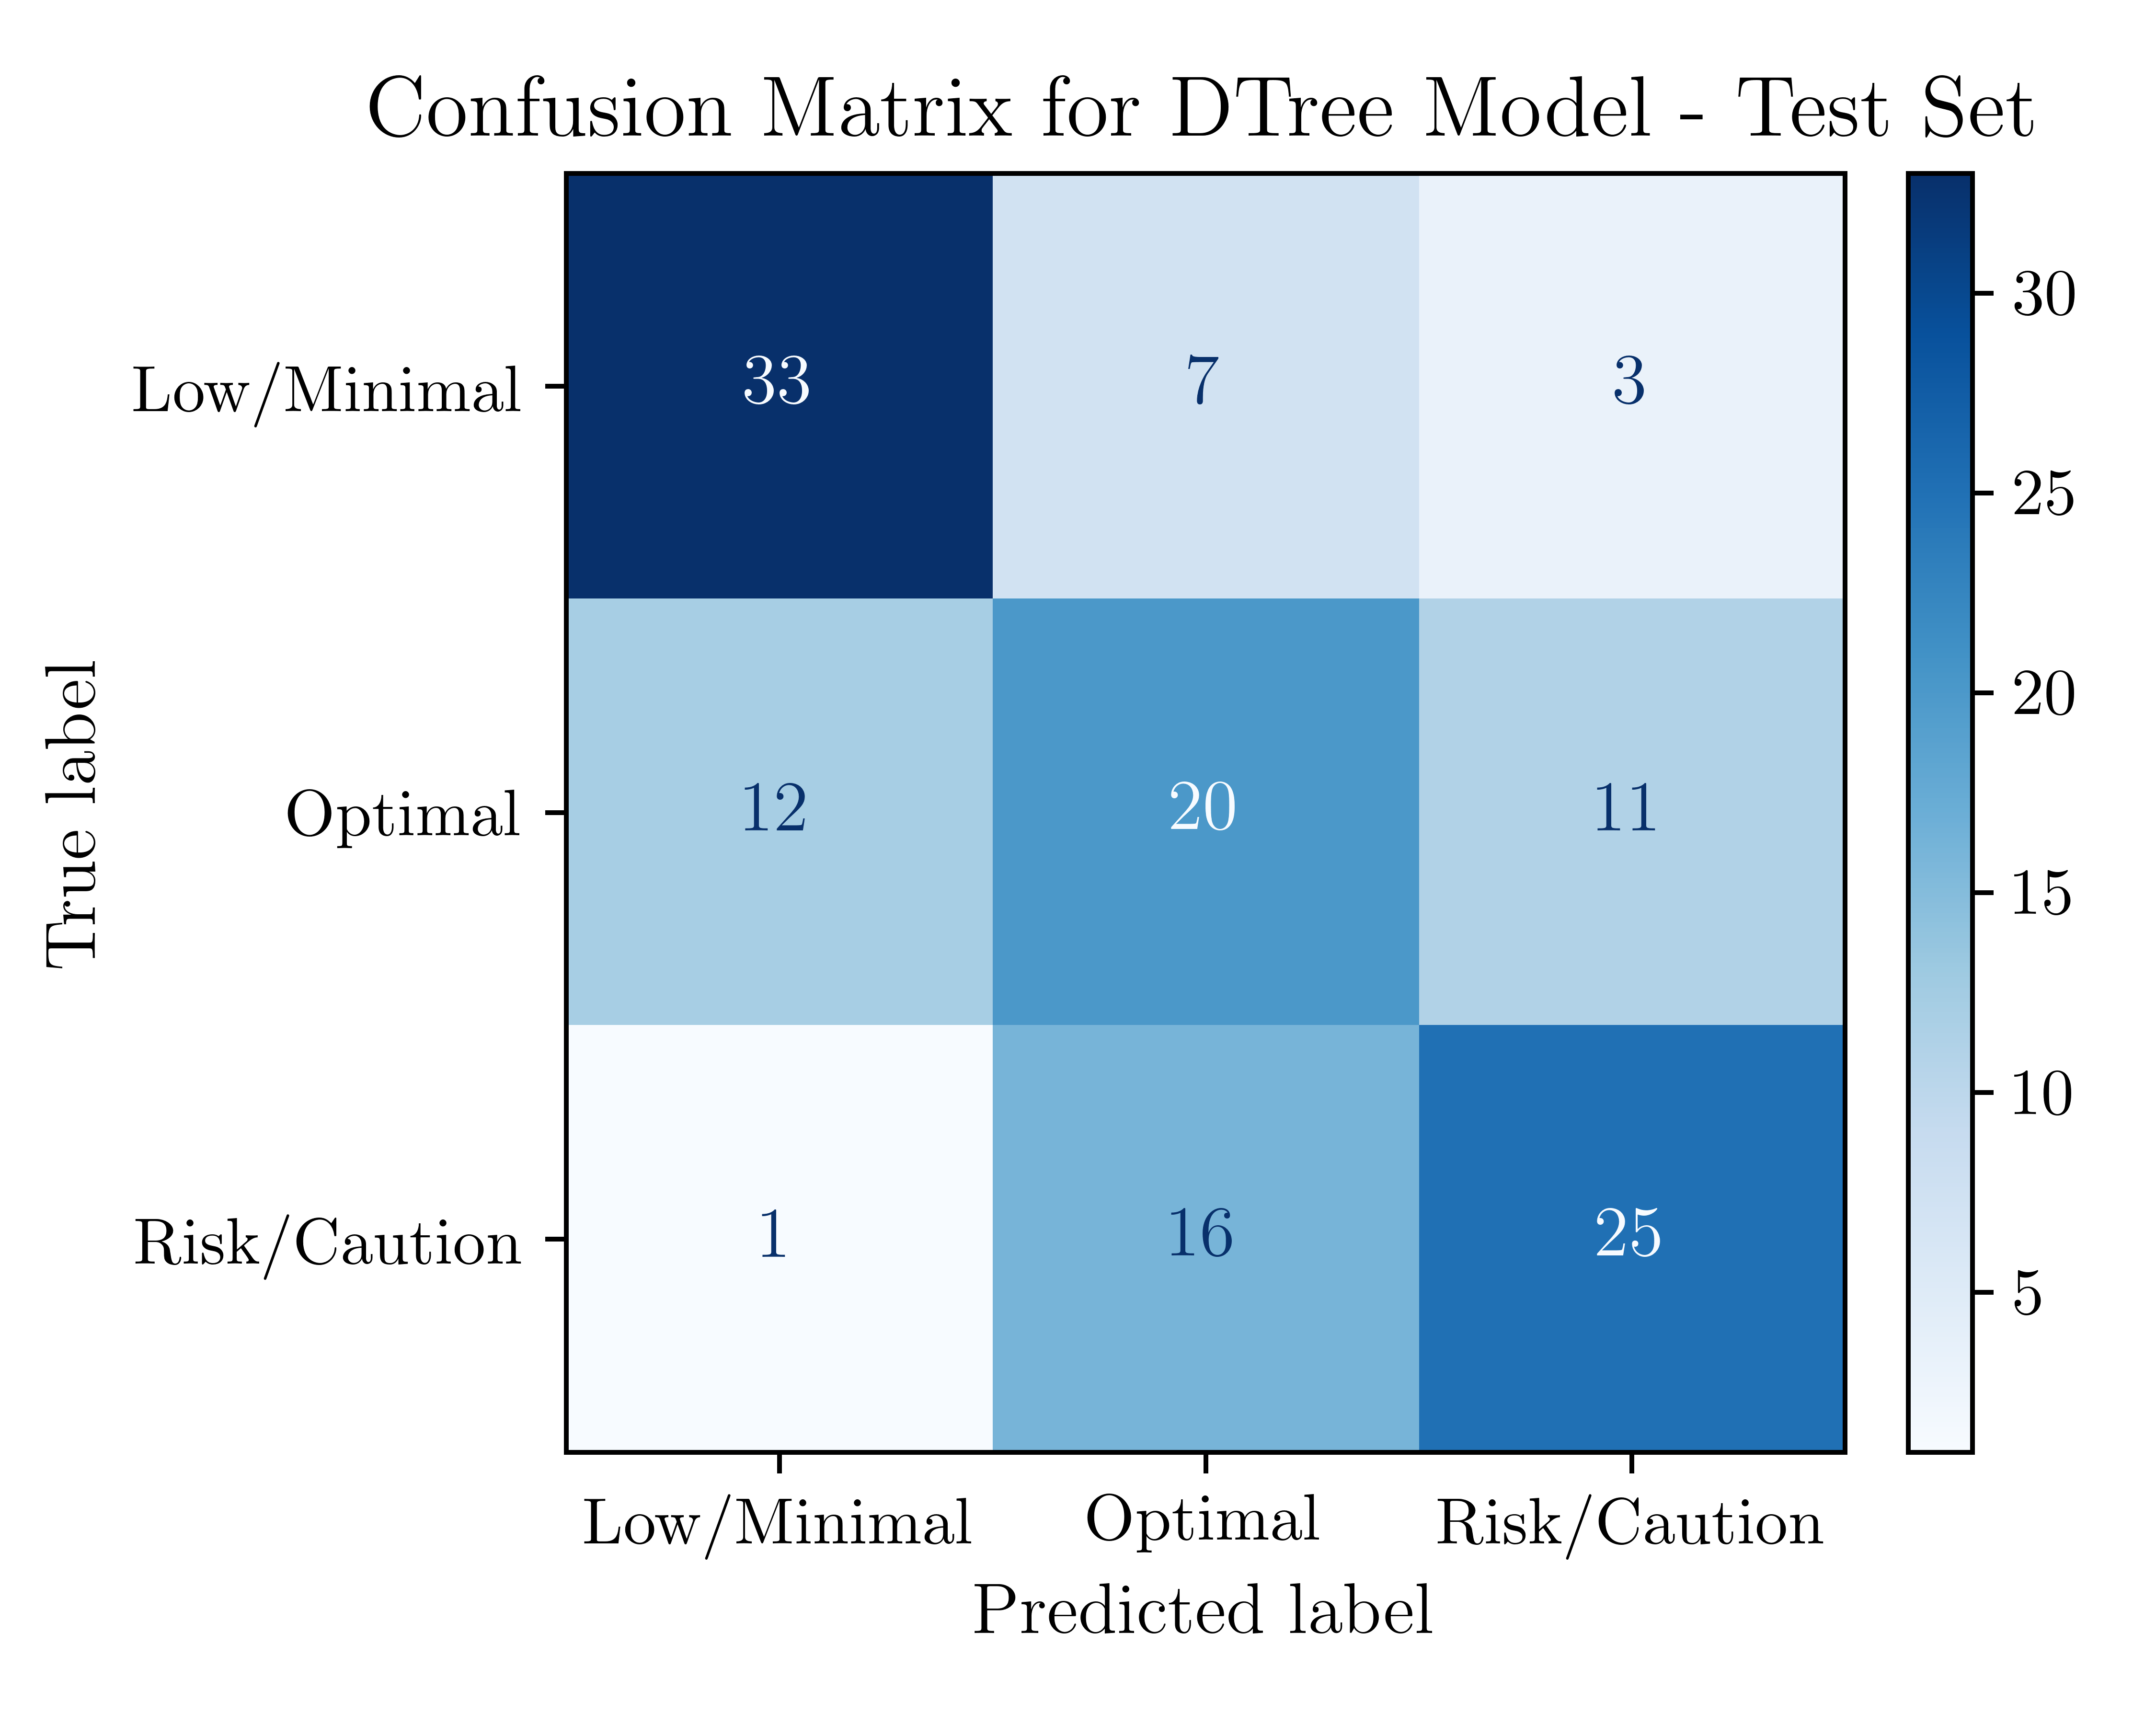
\includegraphics[width=.995\linewidth]{assets/DTREE_ConfusionMatrixTest.png}
    \caption{Evaluation of decision tree model performance on test data performance via confusion matrix.}
    \label{dtree_cmtest}
\end{figure} %cm Test

\begin{table}[H]
\centering
\caption{Classification report for decision tree model performance evaluation on test data.}
\label{cr_dtree_test}
\begin{tabular}{lcccccc}
\toprule
\textbf{Class} & \textbf{Precision} & \textbf{Recall} & \textbf{F1-Score} & \textbf{Support} \\
\midrule
Low/Minimal & 0.72 & 0.77 & 0.74 & 43 \\
Optimal & 0.47 & 0.47 & 0.47 & 43 \\
Risk/Caution & 0.64 & 0.60 & 0.62 & 43 \\
\midrule
\textbf{Accuracy} &  &  & 0.61 & 128 \\
\textbf{Macro avg} & 0.61 & 0.61 & 0.61 & 128 \\
\textbf{Weighted avg} & 0.61 & 0.61 & 0.61 & 128 \\
\bottomrule
\end{tabular}
\end{table} %cr Test



\section{Discussion} \label{discussion_sec}

\subsection{Performance Metrics}

In order to clearly visualize and compare the different models, the results collected were represented using box plots, as depicted in Fig.~\ref{box_plots1}.
The results were obtained from 8-fold cross-validation for the whole dataset in each of the models. In each iteration the models were trained on 7 folds and tested on the eighth. The performance metrics were determined for each iteration and used afterwards to evaluate the global performance of each model. Each model used the optimized hyperparameters described earlier.

\begin{figure}[H]
    \centering
    \begin{subfigure}[1]{\linewidth}
        \centering
        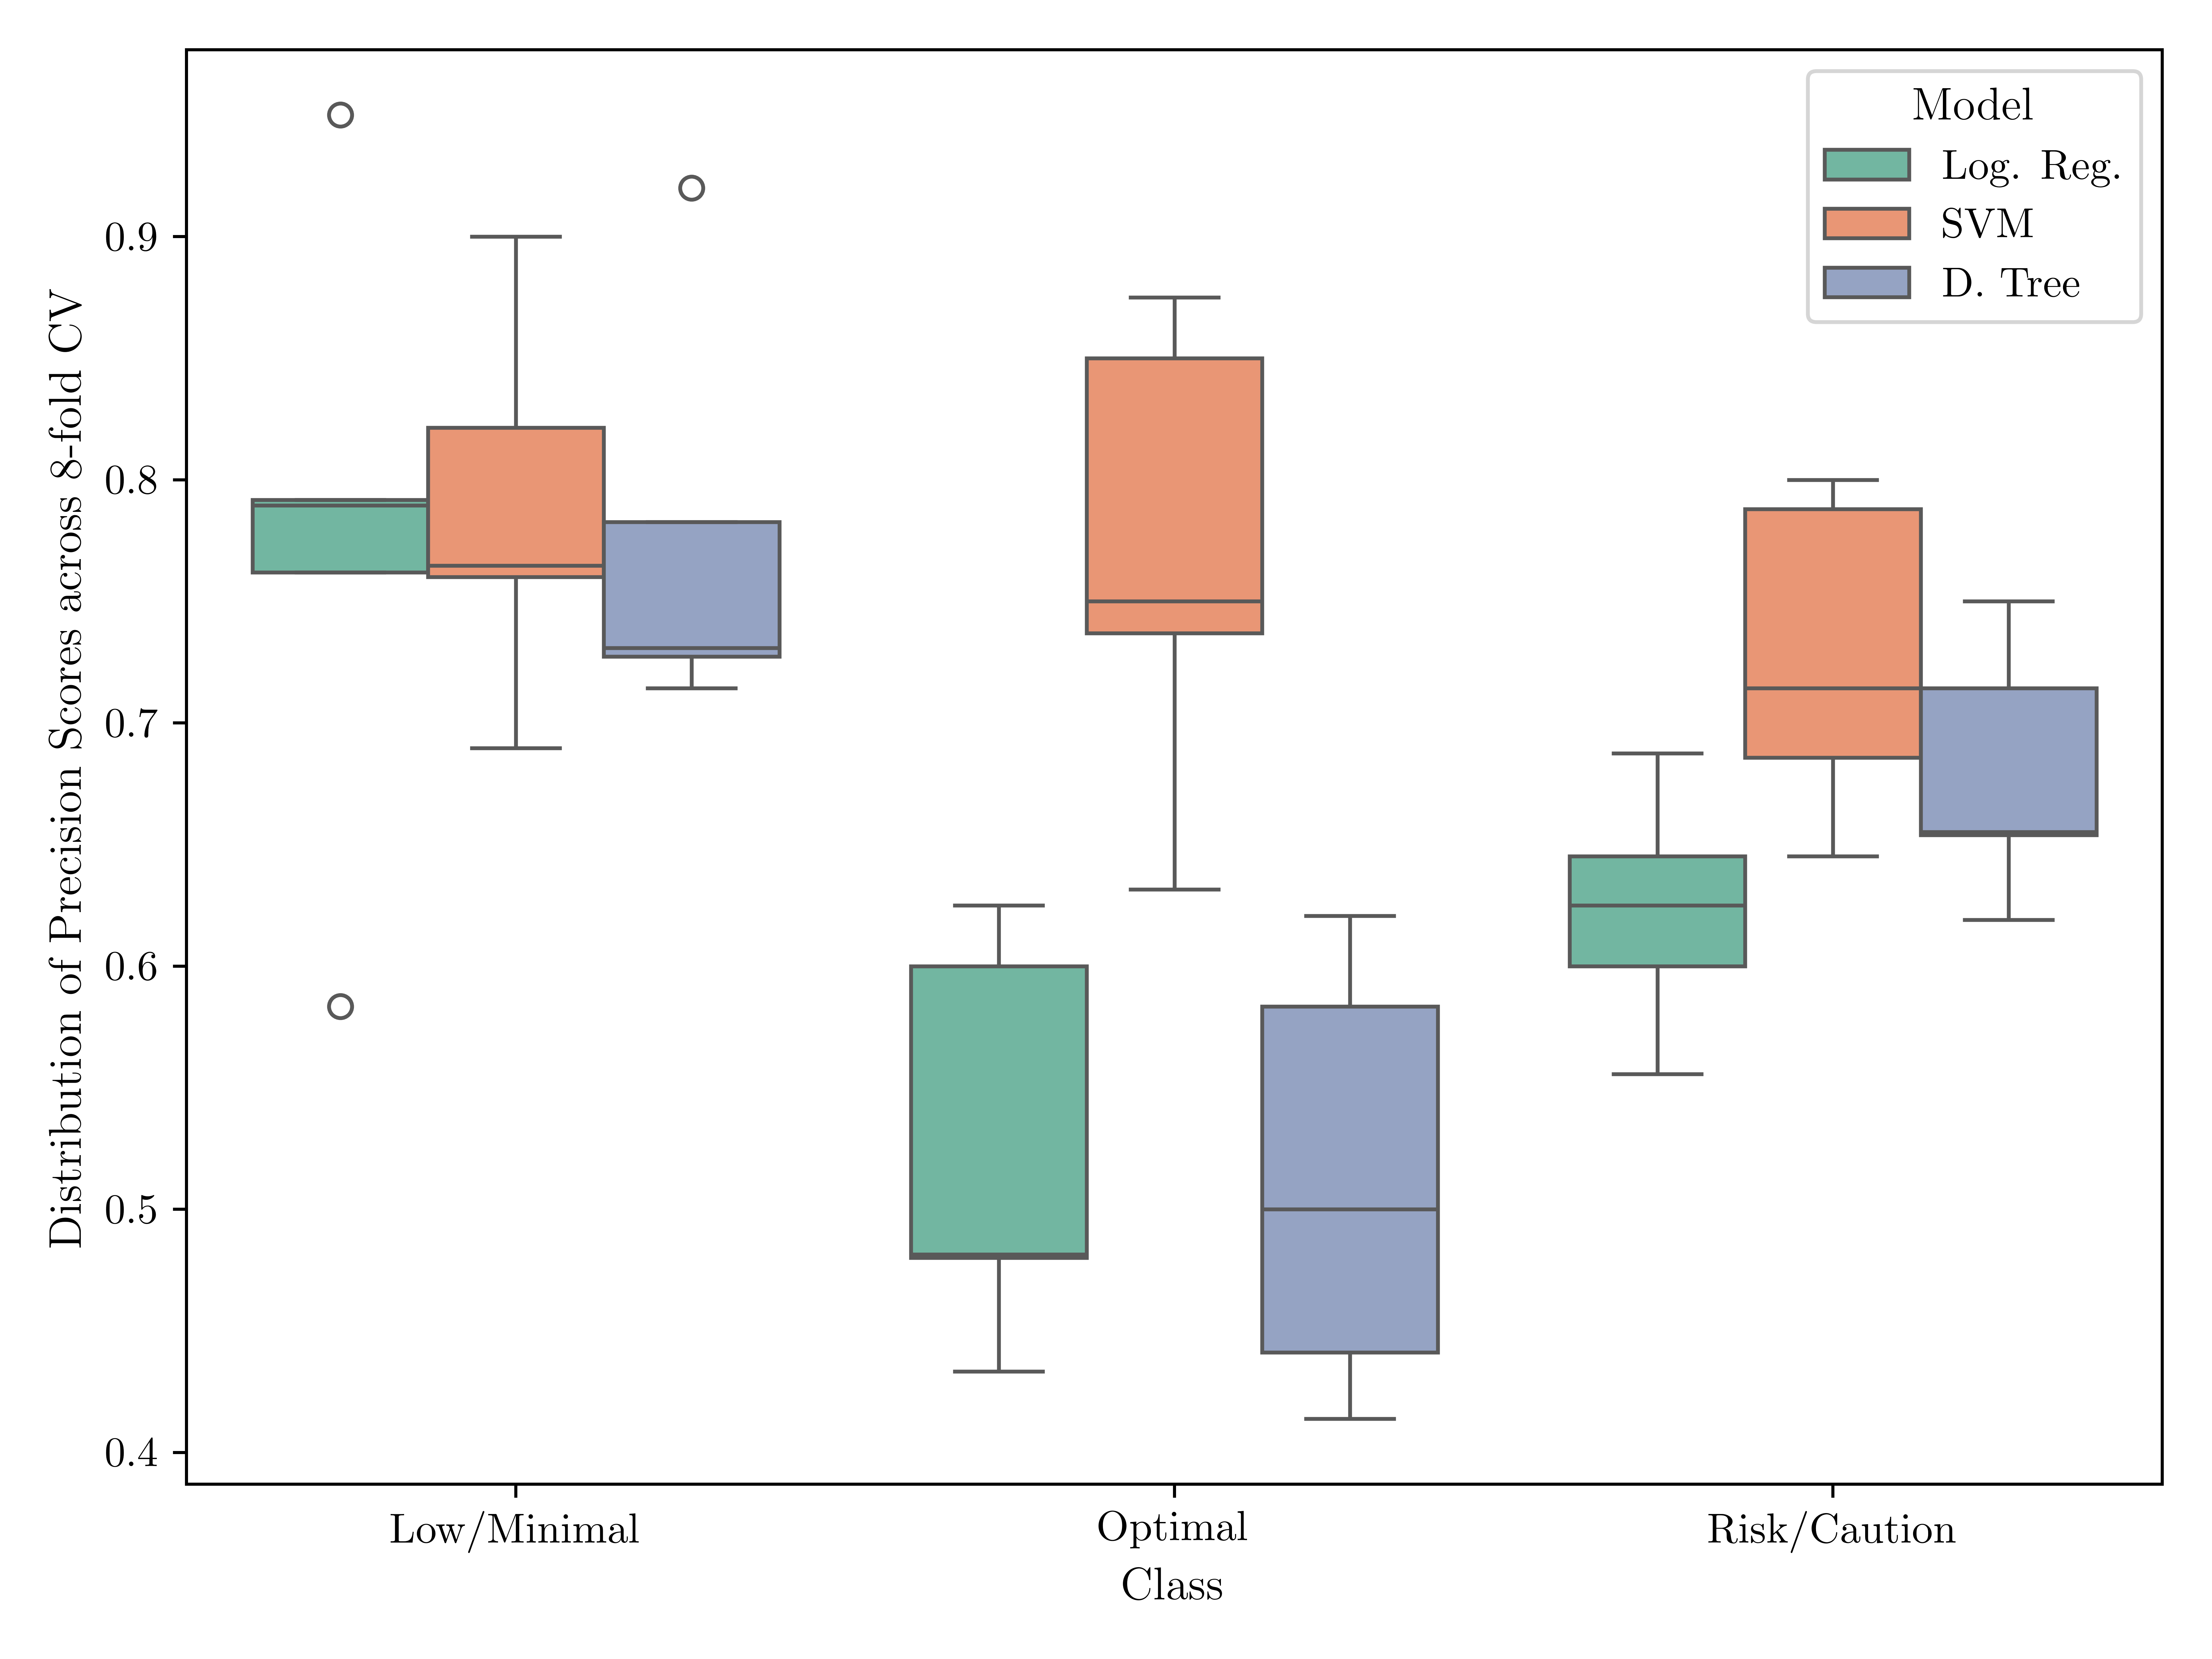
\includegraphics[width=.95\linewidth]{assets/box_precision.png}
        \caption{ }
        \label{box_precision}
    \end{subfigure}
    
    \vspace{0.05cm}

    \begin{subfigure}[1]{\linewidth}
        \centering
        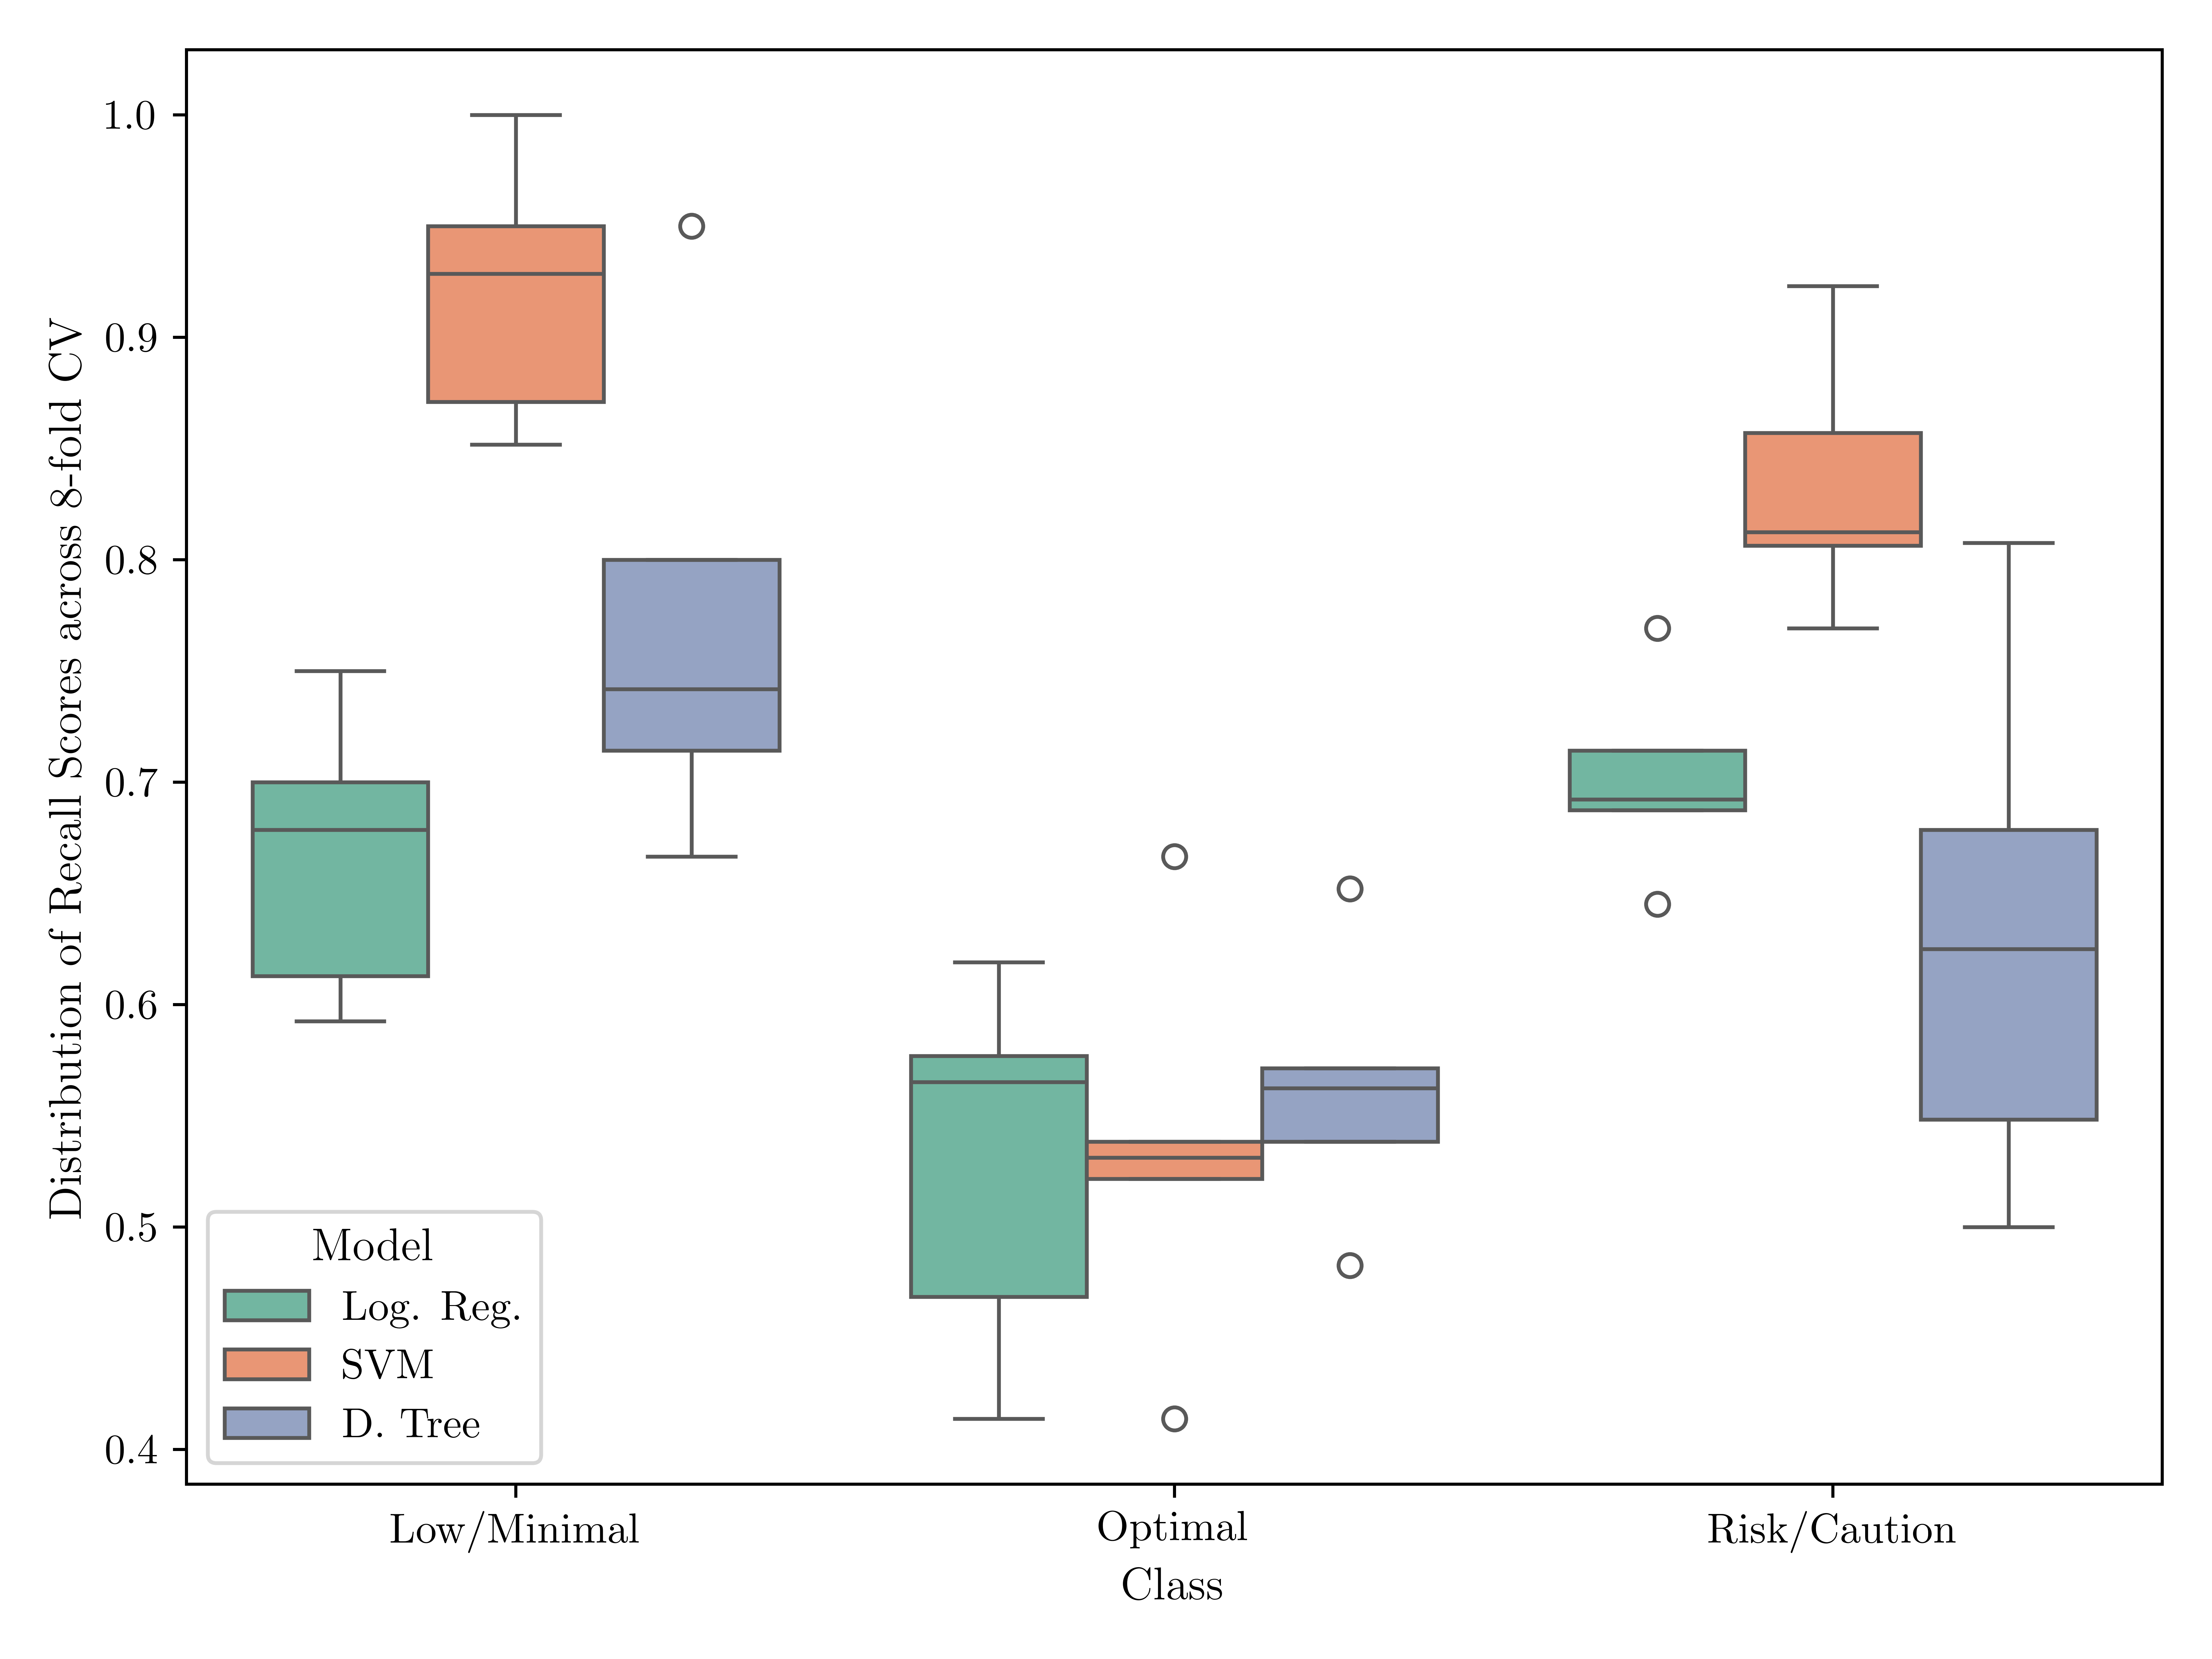
\includegraphics[width=.95\linewidth]{assets/box_recall.png}
        \caption{ }
        \label{box_recall}
    \end{subfigure}
\end{figure}
\begin{figure}[H]
    \ContinuedFloat
    \vspace{0.05cm}

    \begin{subfigure}[1]{\linewidth}
        \centering
        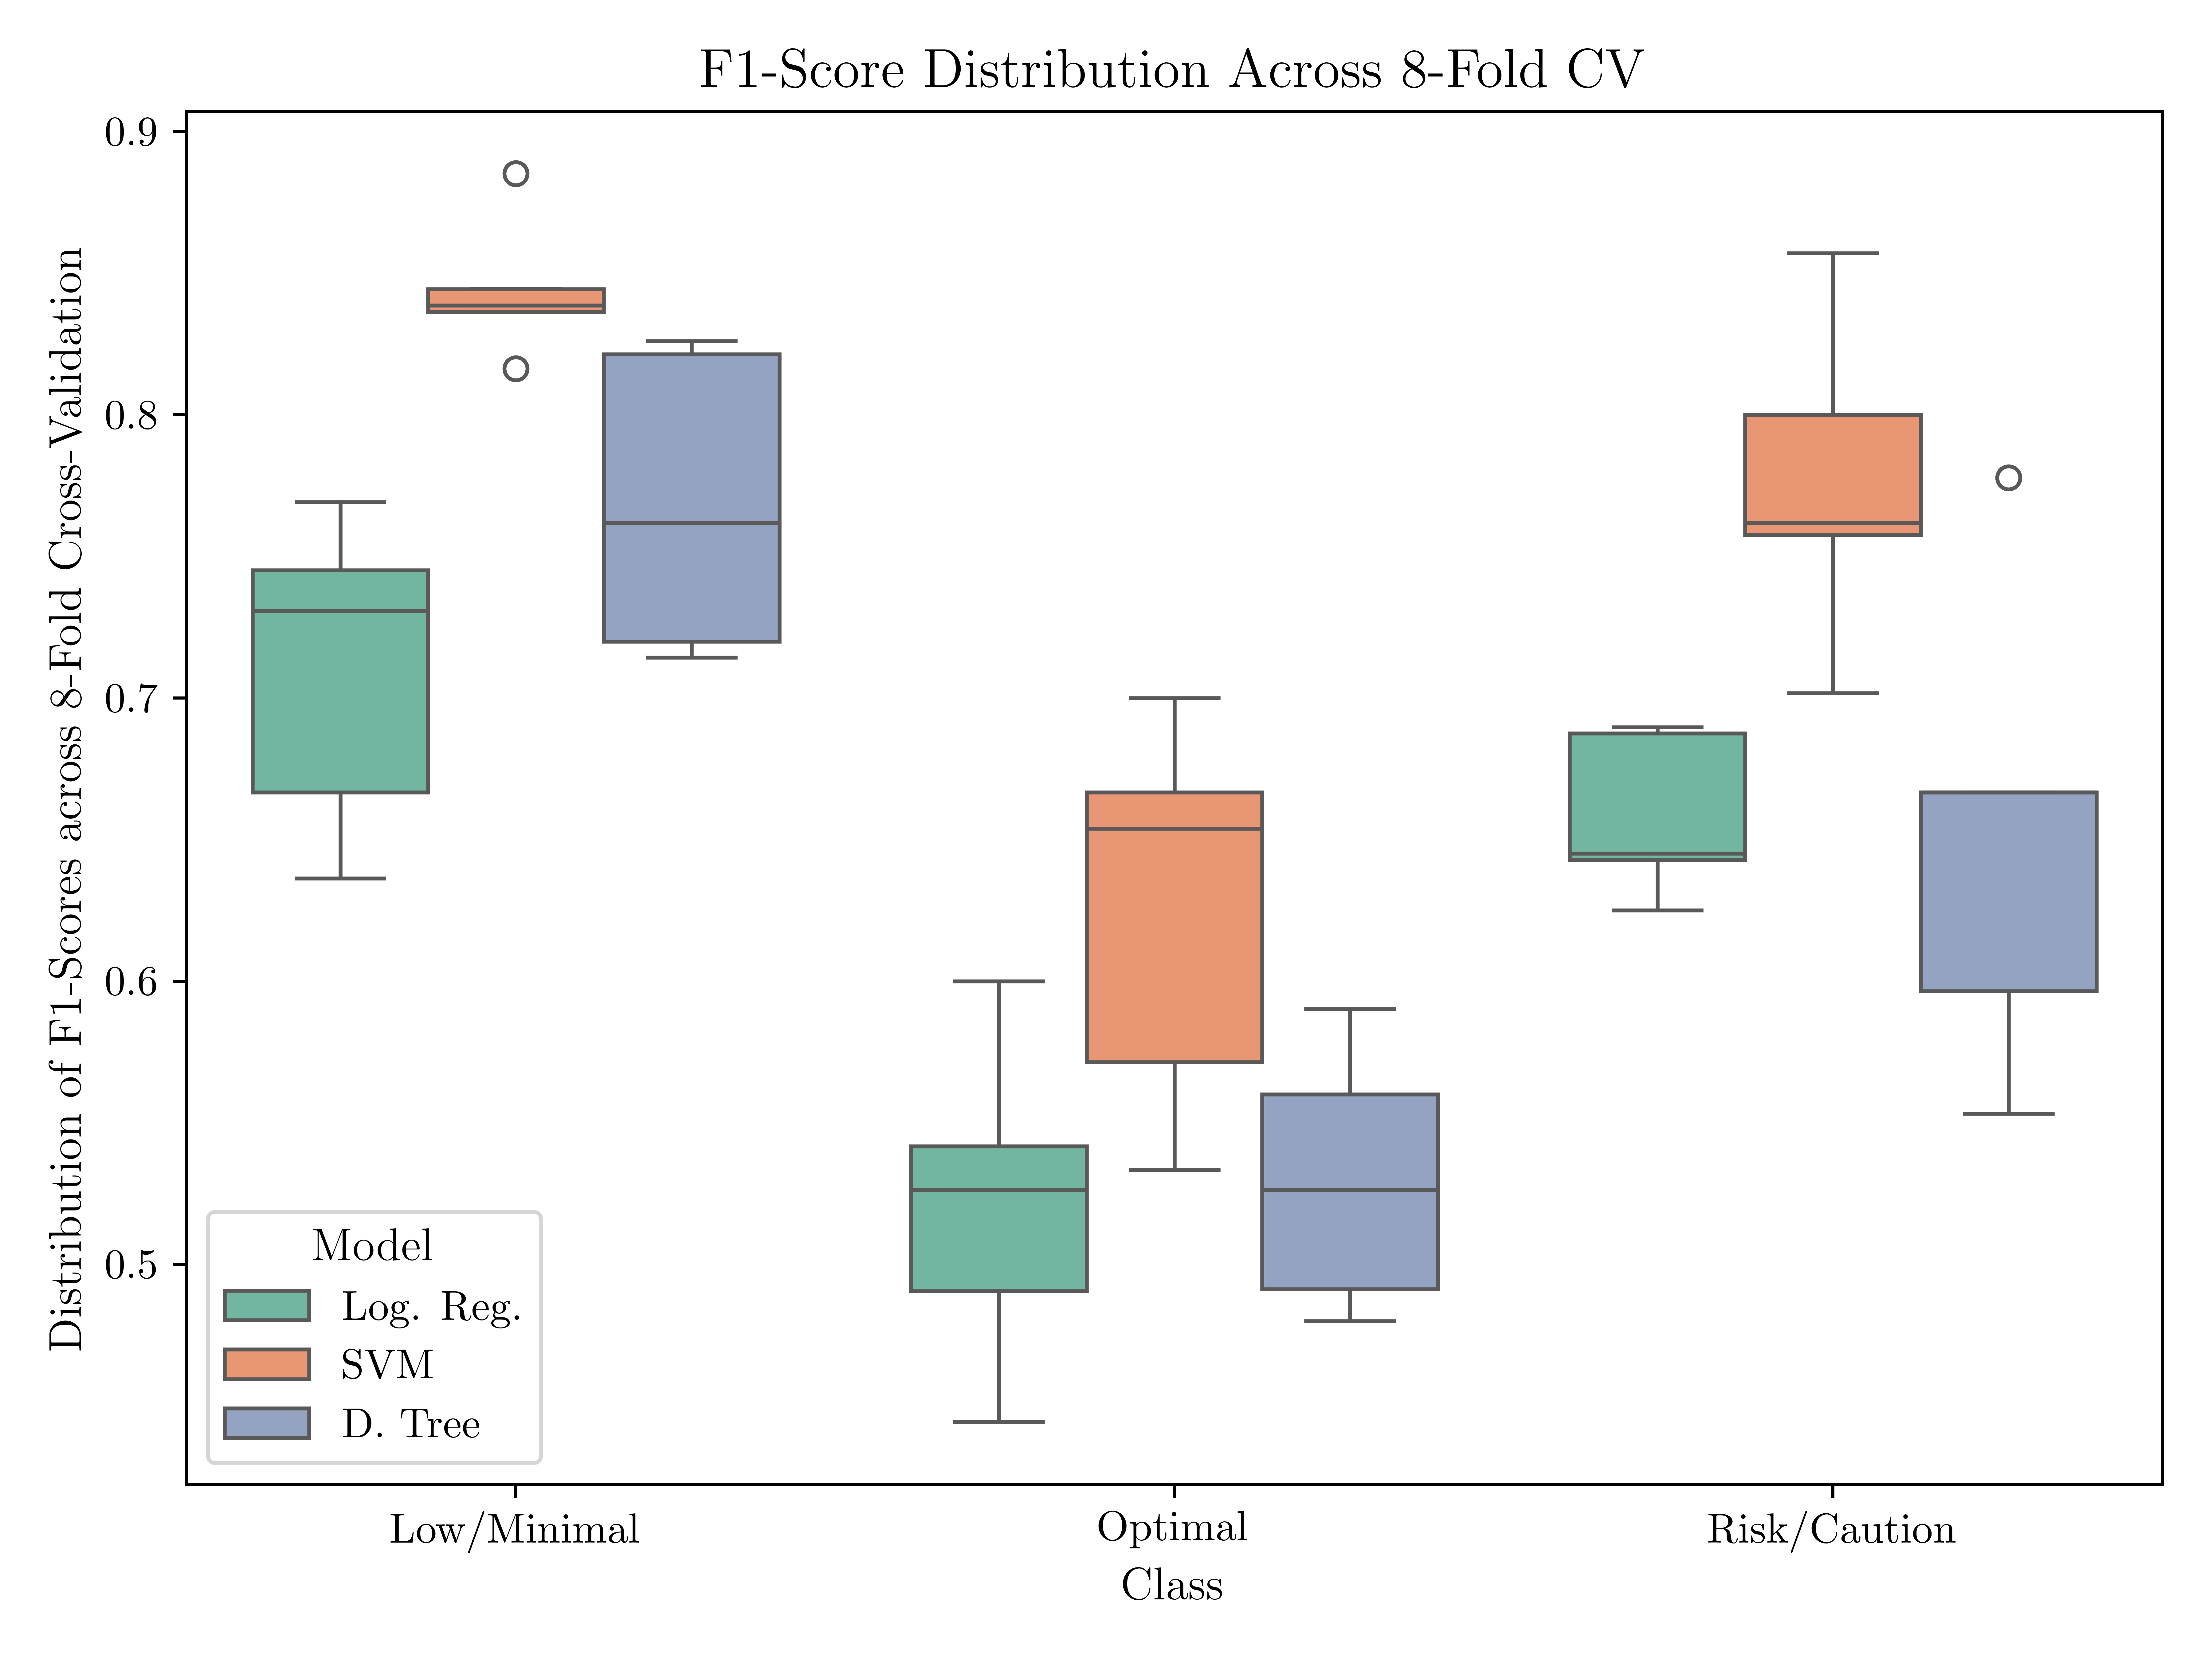
\includegraphics[width=0.95\linewidth]{assets/box_f1score.png}
        \caption{ }
        \label{box_f1score}
    \end{subfigure}
    
    \caption{Boxplots showing the distribution of (a) precision, (b) recall and (c) F1-scores across 8-fold cross-validation for the different classes and models.}
    \label{box_plots1}
\end{figure} %precision, recall, f1

The SVM model stands out with the best performance metrics for all the classes, but the analysis does not end there. The range of scores is not consistently good for any of the models (for some metrics it is narrow with few outliers, most of the times is rather wide). This is a result of the small size of the dataset, where better performing models might be seeing repeated observations from the training to the test dataset, given that the minority class had to have its observations over sampled by duplicating at random some of its observations. For these cases there might be some positive bias, but further analysis of the models would be necessary to confirm to which extent is it happening. The median F1-score for SVM is 0.84 for 'Low/Minimal' class, 0.77 for 'Risk/Caution' with a wider distribution of values, and 0.66 for 'Optimal' with an even wider range. 

The two other models show particularly low values when assessing the sensitivity score, indicating a challenging performance to accurately classify any of the classes (i.e., with a substantial amount of false negatives). The decision tree model fares particularly bad in this aspect, with a spread of possible recall scores from $0.5$ to $0.80$, and 50\% of the values ranging from $0.55$ to $0.65$ for the high stakes class 'Risk/Caution'. However, for the 'Optimal' class none of the models performs adequately: 50\% of the sensitivity scores for LogReg range from $0.48$ to $0.57$, showing that for a good part of the trained models would miss more than 50\% of the true positives, performing worse than guessing at random; SVM and DTree are closer to each other, with the DTree performing slightly better for this class.

For an overall comparison, albeit not ideal,  accuracy scores were computed in the previously described conditions. Both LogReg and DTree perform worse than SVM by more than 10\% for the models' median accuracy, as in Fig.~\ref{box_accuracy}. 

\begin{figure}[H]
    \centering
    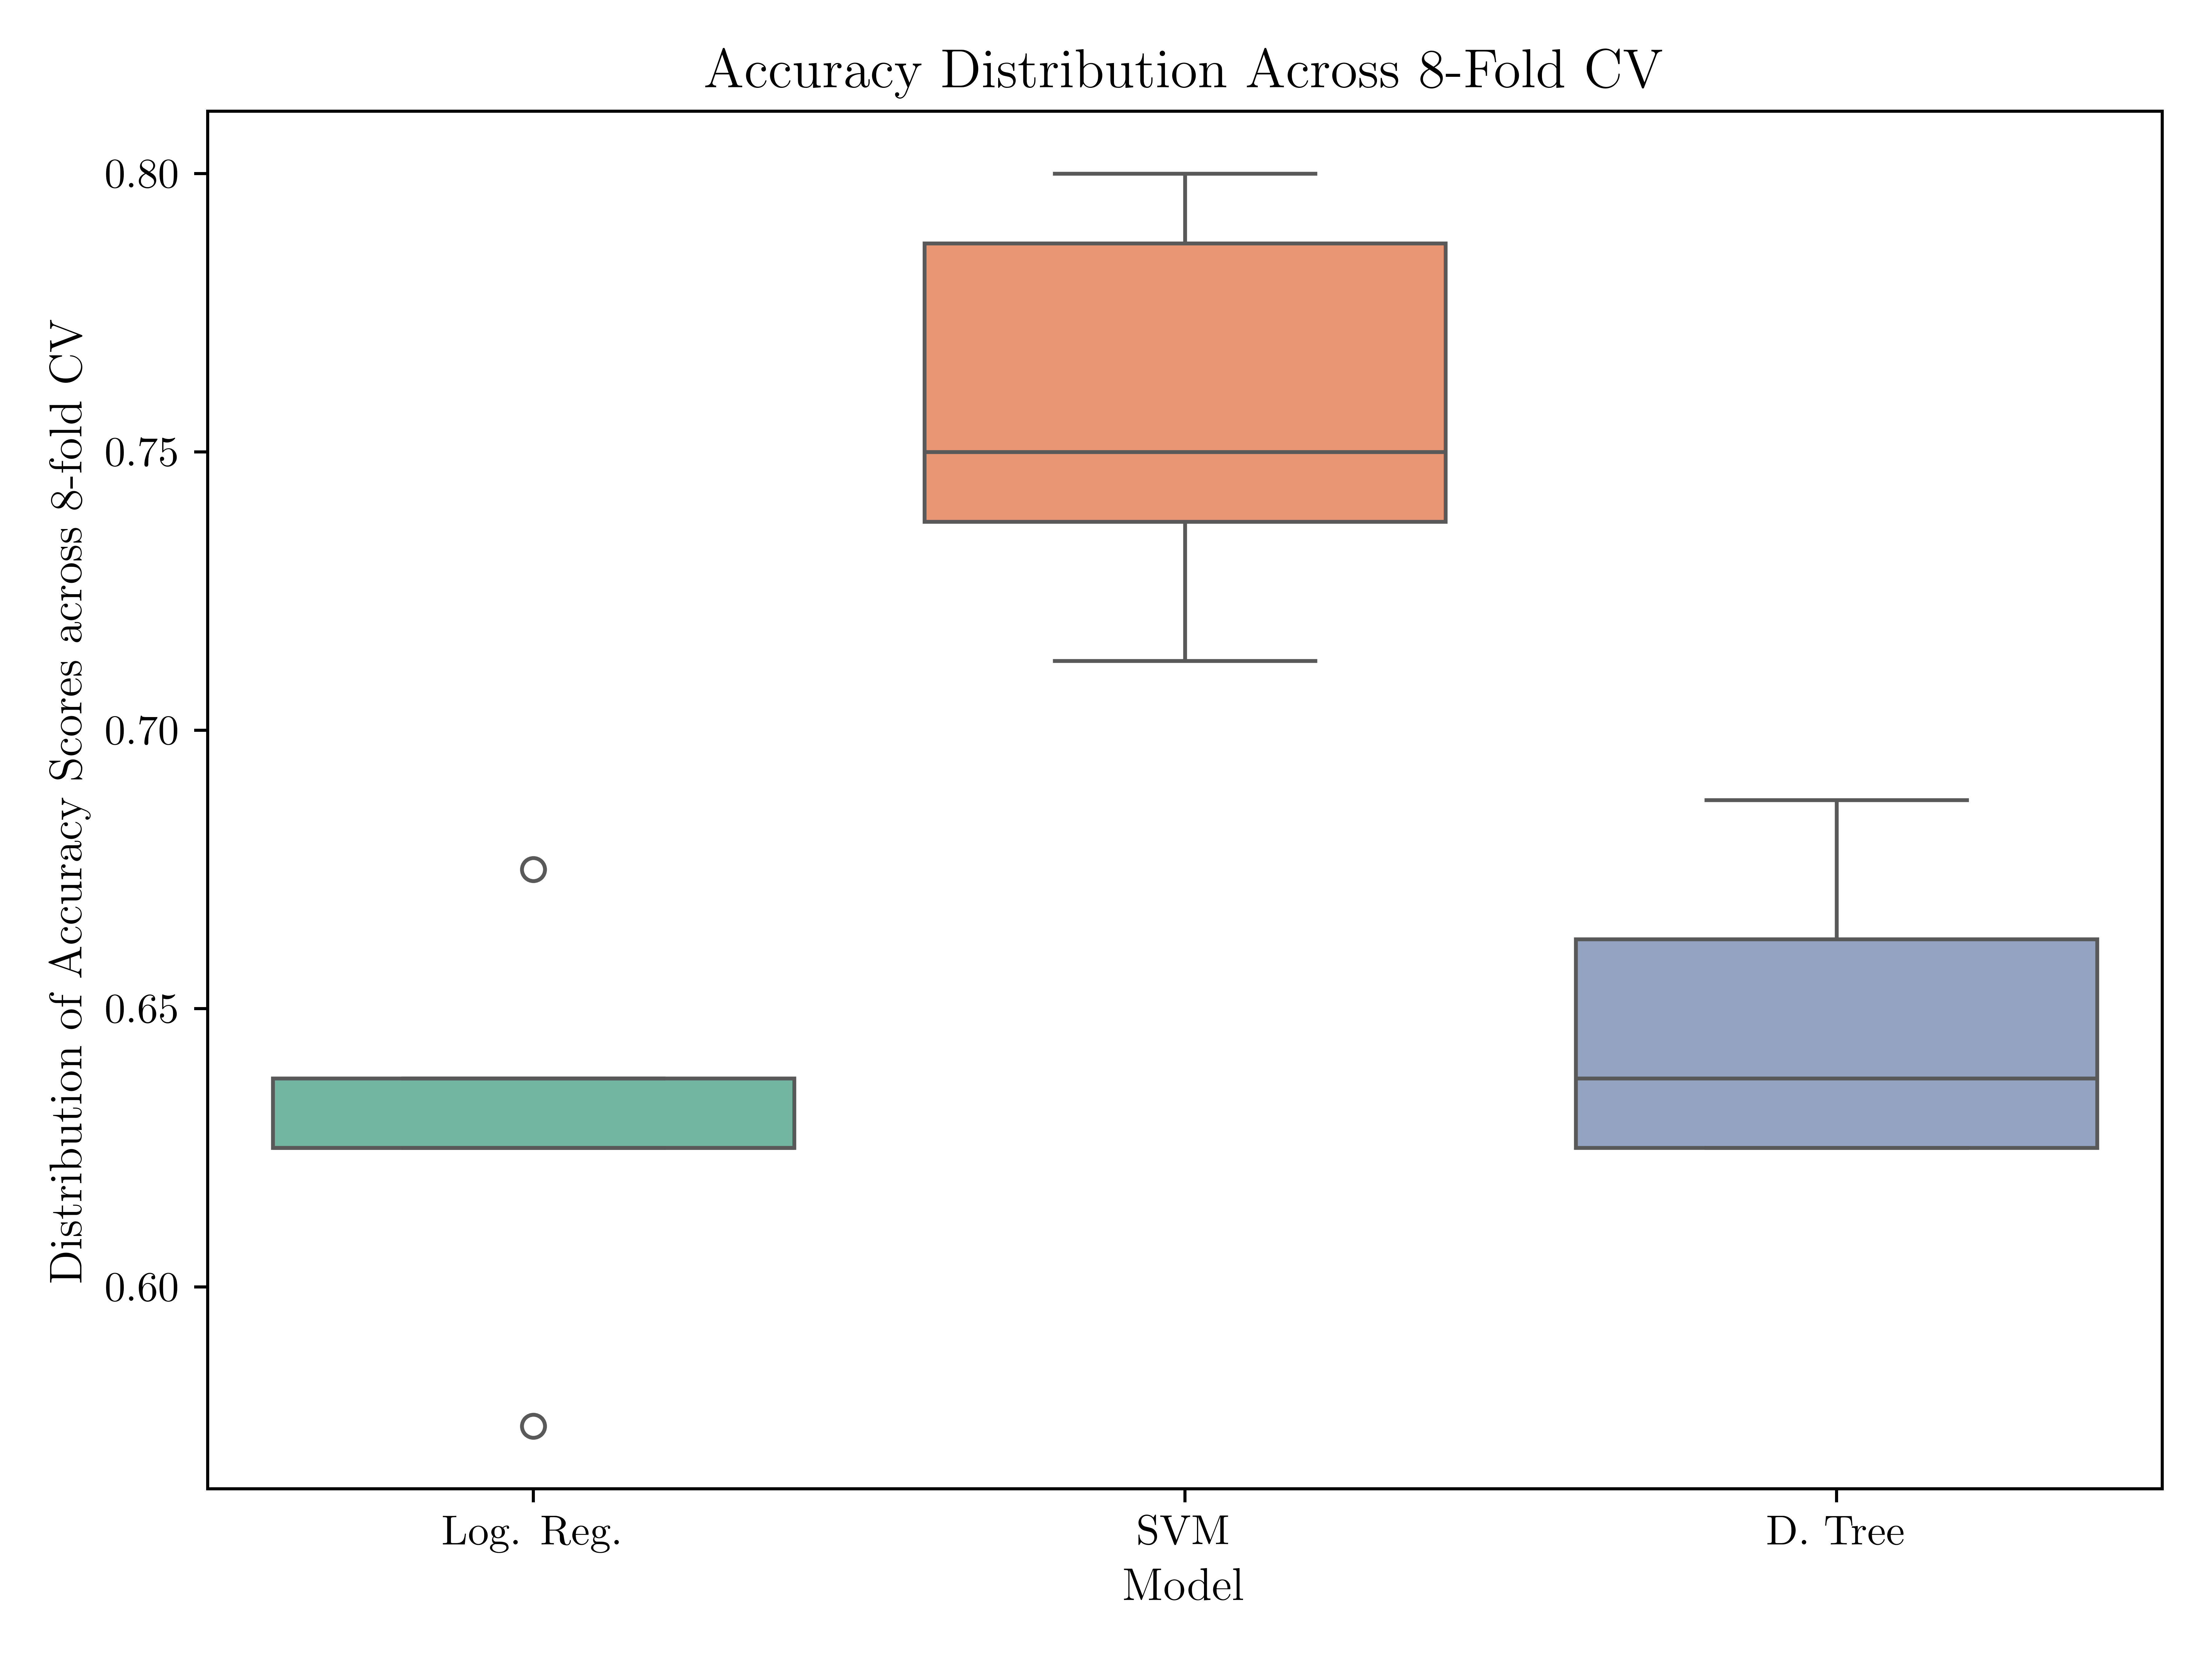
\includegraphics[width=1\linewidth]{assets/box_accuracy.png}
    \caption{Boxplots showing the distribution of accuracy scores across 8-fold cross-validation for different models.}
    \label{box_accuracy}
\end{figure} % accuracy

Nonetheless it is important to keep in mind that accuracy is not the best performance metric for our case for several reasons: class importance, where the misclassification of 'Risk/Caution' class is not penalized (given that it is the most important class to predict accurately); no insight on class performance; random guessing cannot be assessed with no class specific performance.

\subsection{Decision Boundaries}

In order to provide a visual representation of the decision boundaries between the classes, principal component analysis (PCA) was performed for each model on the test dataset. The predicted and real classifications were plotted along the two principal components, each explaining 42.3\% and 26.3\% of the total variance. It is worth reminding that the decision boundaries are an approximation, given that once PCA was applied and only the first two PC were used, roughly 31.4\% of the dataset's variance was lost, meaning that these visualizations are not an accurate representation of the model's performance, but rather a rough estimation.

From the Fig.~\ref{pca_reglog} to \ref{pca_dtree} it is possible to observe the approximation to what the actual decision boundaries are in the space of the principal components. The decision regions are distributed by colors, for LogReg going from 'Low/Minimal' on the left, 'Optimal' center, and 'Risk/Caution' on the right. For SVM and DTree the decision boundaries are more complex, occupying more than one contiguous region.

\begin{figure}[H]
    \centering
    \includegraphics[width=1\linewidth]{assets/pca_reglog.png}
    \caption{Approximation of decision boundaries for logistic regression on principal component axes, showing true and predicted classes.}
    \label{pca_reglog}
\end{figure} % pca logreg

For the LogReg model, the 'Low/Minimal' class shows high precision with several of the true classes correctly placed in the specific region (consistent with the previous analysis and the box plot).

For the remaining classes it seems to be hit or miss for any given point. There's a clear challenge in distinguishing clearly how several of the observations should be classified. 

From the class mapping for the SVM model (Fig.~\ref{pca_svm}) the use of the RBF solver is evident with more complex decision boundaries. These regions provide a more accurate classification, although the region of 'Risk/Caution' shows several observations that should be 'Optimal', evidencing how difficult it is to create a proper decision boundary that would not be an overfitting.

\begin{figure}[H]
    \centering
    \includegraphics[width=1\linewidth]{assets/pca_svm.png}
    \caption{Approximation of SVM decision boundaries on principal component axes, showing true and predicted classes.}
    \label{pca_svm}
\end{figure} % pca svm

\begin{figure}[H]
    \centering
    \includegraphics[width=1\linewidth]{assets/pca_dtree.png}
    \caption{Approximation of decision boundaries for decision tree on principal component axes, showing true and predicted classes.}
    \label{pca_dtree}
\end{figure} % pca dtree

Lastly the DTree model (Fig. \ref{pca_dtree}) displays even more complex decision boundaries, trying to account for the observations that populate the 'Risk/Caution' region. This might be a result of DTree's nature, due to its discrete decisions. Unlike the previous models that need to adjust a continuous surface to separate classes, DTree splits the characteristic space in a hierarchical and discrete fashion given the binary nature of the tree's nodes.

Even though DTree is a powerful ML model to capture non-linear relations, its' graphical interpretation in this context shows the hardships faced to clearly separate observations between classes.

The graphical representations of the models allow to better perceive the complexity behind the problem and the challenges the models face in obtaining an efficient separation between classes. The overlap of classes, especially 'Optimal', shows the need to consider further adjustments to the models, different features for the raw data, or even more robust models that can better capture the relations inherent to the classes.

\subsection{Literature Benchmark}

In the literature the vast majority of work is dedicated to predicting injury. This scenario is strikingly different from the case in study, due to its binary nature (meaning reduced complexity and the tendency to prefer metrics as the area under the curve, AUC, rather than the ones used in this project). Moreover, the studies found while writing the \textit{State of the Art} were related to contact sports (e.g., football, soccer). Nonetheless, the methodology and feature selection is somewhat comparable, despite a clear focus on relying on measurable data (i.e., GPS tracking, smart watches for sleep monitoring, among others). It is also noteworthy that the datasets available in the studies cited are considerably larger, consisting of several athletes (two to three times more than for this project's dataset) and spanning over at least two to three seasons. 

In the work by Ruddy et al. focused on modeling hamstring strain injuries in Australian footballers, where with 10-fold cross-validation the AUC ranged between 0.26 and 0.91 for the best performing model (Näive Bayes) \cite{ruddy2018predictive}. In a different work by Carey et al., the authors modelled the training loads and injury likelihood in Australian footballers. The cross validation was also 10-fold, where the best performing model was regularized LogReg, achieving an AUC of 0.72. Vallance et al. explored the combination of internal and external training loads to predict non-contact injuries in soccer, where the precision and recall for random forest and extreme gradient boosting (XGB) models were close to 0.97 for one-month prediction performance \cite{Carey_2018}.

Despite the different metrics employed, it is safe to assume the best performing model in this project is well within the range of those in the literature. It is important to bear in mind that the target feature for the studies cited (i.e., injury) was measured and based of real observations. In contrast, the fatigue index in the dataset of this project was estimated based on empirical knowledge of the Head Coach. This fact alone highlights the inherent limitations of the original dataset, considering that the fatigue was not actually measured, which is understandable given the complexity and multifaceted nature defining and quantifying what a fatigued state is.

\section{Conclusion}

The objective of this project was to employ different machine learning models to predict the fatigue index in elite swimming athletes, as determined from feedback from athlete's under various forms. The results of this study show that with a reduced dataset, focusing on highly correlated features to fatigue, and careful methodology design it was possible to obtain a well performing model using a support vector machine model. 

Finally, the model will be implemented at the local club, and further work is planned, to improve data collection and feature selection.

\section*{Acknowledgment}

The authors would like to thank Professor Petia Georgieva for her support, fruitful discussions, and for her invaluable slides, which greatly aided in the completion of this project.

Special thanks are also given to Head Coach Daniel Tavares and CAPGE for providing the data and for their encouragement in developing this project.

\section*{Work Load}

Both authors contributed equally to the project.


% trigger a \newpage just before the given reference
% number - used to balance the columns on the last page
% adjust value as needed - may need to be readjusted if
% the document is modified later
%\IEEEtriggeratref{8}
% The "triggered" command can be changed if desired:
%\IEEEtriggercmd{\enlargethispage{-5in}}


\bibliographystyle{IEEEtran}
\bibliography{references}

\end{document}



